%------------------------------------------------------------------
\section{Introduction générale}

Dans les modèles quantiques intégrables, l’évolution vers l’équilibre, à partir d’un état initial arbitraire (et typiquement hors d’équilibre), ne conduit pas à une thermique de Gibbs classique.  
En effet, du fait de l’existence d’une infinité de charges conservées en involution, les systèmes intégrables n’explorent qu’une sous-partie contrainte de l’espace des états accessibles.  
Ils relaxent alors vers un état stationnaire décrit par une \emph{Ensemble Thermodynamique Généralisé} (GGE), qui encode la conservation de toutes ces quantités.

Cette section pose les fondations nécessaires à la description de ces états stationnaires dans le cadre de la \textbf{thermodynamique de Bethe} (TBA), qui généralise l’analyse au-delà de l’état fondamental.  
Nous considérons ici un régime macroscopique à température (ou entropie) finie, correspondant à des états hautement excités du spectre, mais toujours décrits dans le formalisme intégrable exact.

Notre point de départ est la relation constitutive entre la densité de \emph{quasi-particules} (ou rapidités) $\rho(\theta)$ et la densité d’états disponibles $\rho_s(\theta)$, qui encode le spectre accessible en présence d’interactions.  
Nous introduisons ensuite une opération clé de la TBA, appelée \emph{habillage} (\emph{dressing}), qui intervient systématiquement dans le calcul des observables physiques et permet de prendre en compte de manière non perturbative les effets des interactions.  
Cette construction sera illustrée dans le cadre du modèle intégrable de Lieb–Liniger, qui décrit un gaz unidimensionnel de bosons avec interaction delta répulsive.

Les outils développés ici seront fondamentaux pour formuler dans la section suivante le concept d’ensemble généralisé (GGE), et pour décrire la dynamique de relaxation des systèmes intégrables.



\subsection{Notion d’état d’équilibre généralisé (GGE)}

\paragraph{Introduction.}
%Dans les systèmes quantiques intégrables, la dynamique unitaire à long temps ne conduit généralement pas à une thermalisation usuelle, au sens de l’ensemble canonique ou microcanonique. En effet, l'intégrabilité implique l'existence d'une infinité de charges conservées \( \operator{Q}_i \), en involution avec l’Hamiltonien \( \operator{H} \), i.e.
%\begin{eqnarray*}
%[\operator{Q}_i, \operator{H}] = 0,
%\end{eqnarray*}
%et entre elles : \( [\operator{Q}_i, \operator{Q}_j] = 0 \). Ces charges sont localement définies : chacune peut s’écrire sous la forme
%\begin{eqnarray*}
%\operator{Q}_i = \int dx\, \operator{q}_i(x),
%\end{eqnarray*}
%où \( \operator{q}_i(x) \) est une densité locale d’observable (ou "charge locale") à support fini. Cela signifie que pour tout \( i \), la densité \( \operator{q}_i(x) \) est une observable dont le support est contenu dans un sous-domaine borné de l’espace, noté \( \mathcal{S} \subset \mathbb{R} \).

%Cette propriété de localité est essentielle pour décrire l’état du système à l’échelle mésoscopique ou dans un sous-système \( \mathcal{S} \), c’est-à-dire lorsque l’on restreint l’étude à une région finie du système total, typiquement après un processus de relaxation ou de déphasage local. Dans ce cas, le sous-système n’est pas décrit par un état thermique standard (de type Gibbs), mais par une distribution prenant en compte **l’ensemble des charges locales conservées** qui agissent effectivement dans la région \( \mathcal{S} \). Cette construction mène à la notion d’**état d’équilibre généralisé** ou **GGE** (pour *Generalized Gibbs Ensemble*).

%L’état d’équilibre local généralisé est alors défini formellement par une matrice densité de la forme :
%\begin{eqnarray*}
%\operator{\rho}_{\mathcal{S}} = \frac{1}{Z_{\mathcal{S}}} \exp\left( -\sum_i \beta_i\, \operator{Q}_i^{(\mathcal{S})} \right),
%\end{eqnarray*}
%où \( \operator{Q}_i^{(\mathcal{S})} \) désigne la restriction de la charge \( \operator{Q}_i \) à la région \( \mathcal{S} \), c’est-à-dire :
%\begin{eqnarray*}
%\operator{Q}_i^{(\mathcal{S})} = \int_{\mathcal{S}} dx\, \operator{q}_i(x),
%\end{eqnarray*}
%et les coefficients \( \beta_i \in \mathbb{R} \) jouent le rôle de multiplicateurs de Lagrange associés à la conservation des \( \operator{Q}_i \) (on les interprète comme des "potentiels généralisés"). La constante \( Z_{\mathcal{S}} \) est le facteur de normalisation (ou "partition généralisée") :
%\begin{eqnarray*}
%Z_{\mathcal{S}} = \operatorname{Tr} \left[ \exp\left( -\sum_i \beta_i\, \operator{Q}_i^{(\mathcal{S})} \right) \right].
%\end{eqnarray*}

%Ce formalisme permet de décrire l’état macroscopique atteint par un système intégrable après relaxation unitaire, en particulier à la suite d’un *quench* quantique (changement soudain de paramètre). Contrairement à la situation standard où seule l’énergie est conservée, l’ensemble des charges \( \operator{Q}_i \) doit être pris en compte pour correctement prédire les observables locales dans l’état asymptotique.

%L’approche GGE est donc un outil fondamental pour la description de l’équilibre local dans les systèmes intégrables, et permet notamment de comprendre pourquoi la thermalisation habituelle échoue dans ce contexte.

\paragraph{Configuration des états.}\label{sec:config-etats}.
On désigne par $\boldsymbol{\{ \theta_a \}}\equiv \{ \theta_1 , \cdots , \theta_{N} \}$ la \emph{configuration de rapidités} caractérisant un état propre à $N\!=\!N(\boldsymbol{\{ \theta_a \}})$ particules – le nombre de particules n’est donc pas fixé \emph{a priori} mais dépend de la configuration.  
L’état propre correspondant est noté $\ket{\boldsymbol{\{ \theta_a \}}}\;=\;\ket{\{\theta_1,\dots,\theta_N \}}$.

%%%%%%%%%%%%%%%%%%%%%%%%%%%%%%%%%%%%%%%%%%%%%%%%%%
\paragraph{Observables diagonales dans la base des états propres.}
Dans le chapitre précédent (??), on a vu que l'état $\ket{\boldsymbol{\{ \theta_a \}}}$ associé à cette configuration est une fonction propre des observables nombre et moment et  énergie (??). Ces observables sont diagonales dans la base des états propres :
\begin{eqnarray}
	\operator{Q}  =  \sum_{ \{\theta_a\} } \left ( \sum_{a = 1}^{N_a}  1 \right )  \vert \{ \theta_a\}\rangle	\langle \{ \theta_a \}\vert, \, 
	\operator{P}  =  \sum_{\{ \theta_a\}}\left( \sum_{a = 1}^{N_a}  \theta_a \right )   \vert \{ \theta_a\}\rangle	\langle \{ \theta_a \}\vert,\,\operator{H}  =  \sum_{\{ \theta_a\}}\left ( \sum_{a = 1}^{N_a} \frac{\theta_a^2}{2} \right )   \vert \{ \theta_a\}\rangle	\langle \{ \theta_a \}\vert.\label{chap.2.gge.1}		
\end{eqnarray}
avec $ \sum_{\{ \theta_a\}}$ une somme sur tous les configurations.\\
%\begin{eqnarray}
%	\operator{Q} \ket{\{ \theta_a\}}  =  \sum_{ \{\theta_a\} } \left ( \sum_{a = 1}^{N}  1 \right ) \ket{\{ \theta_a\}}, \, 
%	\operator{P} \ket{\{ \theta_a\}}  =  \sum_{\{ \theta_a\}}\left( \sum_{a = 1}^{N}  \theta_a \right ) \ket{\{ \theta_a\}},\,\operator{H} \ket{\{ \theta_a\}}  =  \sum_{\{ \theta_a\}}\left ( \sum_{a = 1}^{N} \frac{\theta_a^2}{2} \right )   \ket{\{ \theta_a\}}.		
%\end{eqnarray}




%%%%%%%%%%%%%%%%%%%%%%%%%%%%%%%%%%%%%%%%%%%%
\paragraph{Contexte et GGE dans les systèmes intégrables.}

Dans un système quantique {\bf intégrable}, il existe une infinité de charges conservées locales $\operator{Q}_i$ commutant entre elles et avec l’Hamiltonien $\operator{H}$ ([Rigol et al. 2007] ) \cite{??}. Concrètement, chaque charge se présente sous la forme $\operator{Q}_i = \int dx \,\operator{q}_i(x)$, où $\operator{q}_i(x)$ est une densité d’observable locale à support borné. L’intégrabilité implique ainsi une caractérisation complète des états propres par un ensemble de paramètres (rapidités $\{\theta_j\}$ dans le modèle de Lieb-Liniger) \cite{??}. En particulier, contrairement aux systèmes génériques, un système intégrable ne thermalise pas au sens canonique classique, car la présence de toutes ces contraintes empêche l’oubli complet des conditions initiales. Les points clés sont alors :

\begin{itemize}[label = $\bullet$]
	\item {\bf Charges conservées} : infinité de locales $\operator{Q}_i$ satisfaisant et $[\operator{Q}_i , \operator{H} ] = 0$ et $[\operator{Q}_i , \operator{Q}_j ] = 0$.
	\item {\bf Densités locales} : chaque $\operator{Q}_i$ s’écrit $\operator{Q}_i = \int_\mathbb{R} dx \, \operator{q}_i(x)$ avec $\operator{q}_i(x)$ à support fini.
	\item {\bf Relaxation non canonique} : après un {\em quench} (changement brutal de paramètre), le système évolue vers un état stationnaire qui n’est pas décrit par l’ensemble canonique habituel.
\end{itemize}

Pour décrire cet état, on introduit l’{\bf ensemble de Gibbs généralisé (GGE)}. Rigol et al. ont montré qu’une « extension naturelle de l’ensemble de Gibbs aux systèmes intégrables » prédit correctement les valeurs moyennes des observables après relaxation \cite{??}.  Formellement, pour une région finie du système $\mathcal{S} \subset \mathbb{R}$, on définit la matrice densité locale :
\begin{eqnarray}
	\operator{\rho}^{(\mathcal{S})}_{\mathrm{GGE}} = \frac{1}{Z^{(\mathcal{S})}}\exp \left ( - \sum_i \beta_i \operator{Q}_i^{(\mathcal{S})} \right), \quad \operator{Q}_i^{(\mathcal{S})} = \int_\mathcal{S} dx \, \operator{q}_i(x), \label{chap.TBA.op.rho.S}	
\end{eqnarray}

où $\beta_i \in \mathbb{R}$ sont les multiplicateurs de Lagrange (ou « températures généralisées ») associés aux charges locales conservées $\{\operator{Q}_i\}$. La fonction de partition $Z^{(\mathcal{S})} = \bm{\mathrm{Tr}}[\exp ( - \sum_i \beta_i \operator{Q}_i^{(\mathcal{S})} ) ]$ assure la normalisation. L’{\bf état GGE} ainsi défini est le seul permettant de prédire de manière cohérente les observables locales de $\mathcal{S}$ à long temps \cite{??}. Autrement dit, l’équilibre local après quench est un état stationnaire faisant perdurer la mémoire de chaque charge conservée, ce qui conduit à un nombre macroscopique de paramètres $\beta_i$ thermodynamiques (une « température » par charge) \cite{??}.

 \subparagraph{Interprétation des multiplicateurs de Lagrange.}
Les multiplicateurs de Lagranges $\beta_i$ apparaissent naturellement lors de l'optimisation sous contraintes, par exemple dans le formalisme de l'{\bf ensemble de Gibbs généralisé (GGE)}, oû il imposent la conservation des valeurs moyennes des charges $\langle \operator{Q}_i^{(\mathcal{S})} \rangle_{\operator{\rho}^{(\mathcal{S})}_{\mathrm{GGE}}} = \bm{\mathrm{Tr}}[\operator{\rho}^{(\mathcal{S})}_{\mathrm{GGE}} \operator{Q}_i^{(\mathcal{S})}]   $.\\

En résumé, la GGE généralise les ensembles canoniques standard : au lieu de retenir uniquement l’énergie, on impose la conservation de l’ensemble complet $\{\operator{Q}_i \}$. Cette construction rend compte du fait que, dans un système intégrable, les observables locaux convergent vers les valeurs moyennes de $\operator{\rho}^{(\mathcal{S})}_{\mathrm{GGE}}$ , et non vers celles d’un Gibbs thermique ordinaire \cite{??}\cite{??}. On comprend ainsi pourquoi la {\em thermalisation habituelle} (canonique ou microcanonique) échoue : seul l’ensemble de Gibbs généralisé peut intégrer toutes les contraintes locales.

\paragraph{Rappel sur le modèle de Lieb-Liniger et distribution de rapidités.}
Comme rappelé au chapitre précédent, {\bf le modèle de  Lieb-Liniger} (gaz bosonique 1D à interactions de contact) est un exemple paradigmatique d’un système intégrable \cite{??}. Ses états propres sont caractérisés par un ensemble de $N$  rapidités $\{ \theta_a \}$ , qui jouent le rôle de quasi-momenta ({\bf Bethe ansatz}). Dans ce contexte, l’état macroscopique du gaz après relaxation unitaire est entièrement déterminé par la {\bf distribution des rapidités}. Formellement, on définit $\rho(\theta)$ la distribution intensive des rapidités telle que $\rho(\theta) d \theta$ donne la fraction de particules par unité de longueur ayant une rapidité dans la cellule $[\theta , \theta + d \theta ] $.\\

Cette « distribution de rapidités » est d’autant plus pertinente qu’elle est {\em accessible expérimentalement}. En effet, lorsque le gaz bosonique 1D est libéré et laissé s’étendre, la distribution asymptotique des vitesses des atomes coïncide avec la distribution initiale des rapidités \cite{??} . Autrement dit, la GGE prédit un profil de vitesses observables en laboratoire. Léa Dubois souligne dans sa thèse que " la distribution de rapidités est la distribution asymptotique des vitesses des atomes après une expansion dans le guide 1D ", et qu’elle peut être extraite par l’hydrodynamique généralisée \cite{??}. \\

Dans la GGE, cette distribution macroscopique $\rho(\theta)$ est fixée par l’ensemble des charges conservées. Par exemple, on ajuste les $\beta_i$ de sorte que les valeurs moyennes $\langle \operator{Q}_i \rangle_{\operator{\rho}^{(\mathcal{S})}_{\mathrm{GGE}}}$ correspondent aux valeurs initiales. Ce processus détermine donc la fonction $\rho(\theta)$ décrivant l’état d’équilibre local. Les observables locaux du gaz (densité, corrélations, etc.) en découlent alors via les équations de Bethe ansatz. 

%%%%%%%%%%%%%%%%%%%%%%%%%%%%%%%%%%%%%%%%%%%%%%%%%%
\paragraph{Charges conservées locales diagonales dans la base des états propres.}
Les charges conservées locales $\operator{Q}_i^{(\mathcal{S})}$ est diagonale dans la base des  états propres $\ket{ \{ \theta_a \}}$ , avec pour valeurs propres $\langle \operator{Q}_i^{(\mathcal{S})} \rangle_{\{\theta_a \}} = \bm{\mathrm{Tr}}[\ket{\{\theta_a \}}\!\bra{\{\theta_a \}} \operator{Q}_i^{(\mathcal{S})}] =  \bra{\{\theta_a \}} \operator{Q}_i^{(\mathcal{S})} \ket{\{\theta_a \}}$ :
%\begin{eqnarray}
%	\operator{Q}_i^{(\mathcal{S})} & = & \sum_{ \{\theta_a\} } \langle \operator{Q}_i^{(\mathcal{S})} \rangle_{\{\theta_a \}}  \ket{\{\theta_a \}}\!\bra{\{\theta_a \}}.		
%\end{eqnarray}
\begin{eqnarray}
	\operator{Q}_i^{(\mathcal{S})}\ket{\{\theta_a \}} & = &  \langle \operator{Q}_i^{(\mathcal{S})} \rangle_{\{\theta_a \}}  \ket{\{\theta_a \}}.		
\end{eqnarray}
%%%%%%%%%%%%%%%%%%%%%%%%%%%%%%%%%%%%%%%%
\paragraph{Probabilité d’un état à rapidités fixées.}
On peut alors définir la probabilité d’occurrence d’un état $\ket{\{ \theta_a \} }$ :
\begin{eqnarray}
	\mathbb{P}^{(\mathcal{S})}_{\{ \theta_a \}}  =  \bm{\mathrm{Tr}} \left [\operator{\rho}^{(\mathcal{S})}_{\mathrm{GGE}} \ket{\{\theta_a \}}\!\bra{\{\theta_a \}} \right ] =  \bra{\{\theta_a \}}	\operator{\rho}^{(\mathcal{S})}_{\mathrm{GGE}} \ket{\{\theta_a \}}  = \frac{1}{Z^{(\mathcal{S})}} \exp \left (- \sum_i \beta_i \langle \operator{Q}_i^{(\mathcal{S})} \rangle_{\{\theta_a \}} \right ) .
\end{eqnarray}

%%%%%%%%%%%%%%%%%%%%%%%%%%%
\paragraph{Moyenne d’un charges conservées locales et dérivées de $Z^{(\mathcal{S})}$.}
On peut écrire la moyenne d’une observable comme une somme pondérée par cette probabilité, ou encore comme une dérivée de la fonction de partition :
\begin{eqnarray}
	\langle \operator{Q}_i^{(\mathcal{S})} \rangle_{\operator{\rho}^{(\mathcal{S})}_{\mathrm{GGE}}} &= & \sum_{\{ \theta_a\}} \langle \operator{Q}_i^{(\mathcal{S})} \rangle_{\{\theta_a \}} \mathbb{P}^{(\mathcal{S})}_{\{ \theta_a \}} ~=~- \left. \frac{1}{Z^{(\mathcal{S})}} \frac{\partial Z^{(\mathcal{S})}}{\partial \beta_i} \right )_{\beta_{j \neq i }} ~=~ - 	\left . \frac{\partial  \ln Z^{(\mathcal{S})}}{\partial \beta_i} \right )_{\beta_{j \neq i }}	
\end{eqnarray}

Par le même raisonnement la moyenne de $(\operator{Q}_i^{(\mathcal{S})})^n$ s'écrit :

\begin{eqnarray}
	\langle (\operator{Q}_i^{(\mathcal{S})})^n \rangle &= & \sum_{\{ \theta_a\}} (\langle\operator{Q}_i^{(\mathcal{S})}\rangle_{\{\theta_a\}})^n \mathbb{P}^{(\mathcal{S})}_{\{ \theta_a \}} ~=~ (-1)^n \left. \frac{1}{Z^{(\mathcal{S})}} \frac{\partial^n Z^{(\mathcal{S})}}{{(\partial \beta_i)}^n} \right )_{\beta_{j \neq i }} .	
\end{eqnarray}

%%%%%%%%%%%%%%%%%%%%%%%%%%%%%%%
\paragraph{Moments d’ordre supérieur et fluctuations.}
Le premier et second moments permettent d’accéder à la variance de l’observable :
\begin{eqnarray}
	\Delta_{\operator{Q}_i^{(\mathcal{S})}}^2 &=&  	\left \langle \left (\operator{Q}_i^{(\mathcal{S})} - \langle\operator{Q}_i^{(\mathcal{S})} \rangle_{\operator{\rho}^{(\mathcal{S})}_{\mathrm{GGE}}} \right )^2  \right \rangle_{\operator{\rho}^{(\mathcal{S})}_{\mathrm{GGE}}}  = 	\langle(\operator{Q}_i^{(\mathcal{S})})^2 \rangle_{\operator{\rho}^{(\mathcal{S})}_{\mathrm{GGE}}}  -  \langle\operator{Q}_i^{(\mathcal{S})} \rangle_{\operator{\rho}^{(\mathcal{S})}_{\mathrm{GGE}}}^2 \nonumber  \\
		& = & \left . \frac{1}{Z^{(\mathcal{S})}} \frac{ \partial^2 Z^{(\mathcal{S})} }{ {\partial \beta_i}^2 }  \right )_{\beta_{j\neq i}} - \left ( \left . \frac{1}{Z}\frac{ \partial Z^{(\mathcal{S})} }{ \partial \beta_i }  \right )_{\beta_{j\neq i}}\right )^2     \nonumber\\
		&=&  \frac{\partial}{\partial \beta_i } \left ( \left . \frac{1}{Z^{(\mathcal{S})}} \frac{\partial Z^{(\mathcal{S})}}{\partial \beta_i }  \right )_{\beta_{j\neq i}}  \right )_{\beta_{j\neq i}} \nonumber \\
		&=&	  \left . \frac{\partial^2 \ln Z^{(\mathcal{S})}  }{{\partial \beta_i}^2 }  \right )_{\beta_{j\neq i}} =  - \left . 	\frac{\partial \langle\operator{Q}_i^{(\mathcal{S})} \rangle_{\operator{\rho}^{(\mathcal{S})}_{\mathrm{GGE}}} }{\partial \beta_i } \right )_{\beta_{j\neq i}}.	
\end{eqnarray}

%%%%%%%%%%%%%%%%%%%%%%%%%%%%%%
\paragraph{Cas particulier de l’équilibre thermique.}

Dans le cas particulier de l’équilibre thermique standard (i.e. Gibbsien), le système est décrit par une seule contrainte d’énergie (ou d’énergie et de particule, dans le cas d’un grand canonique). Les multiplicateurs de Lagrange associés aux charges conservées peuvent alors être identifiés à des grandeurs thermodynamiques classiques.

\begin{itemize}[label=$\bullet$]
	\item Si la seule charge conservée est le nombre de particules $\operator{Q}_0^{(\mathcal{S})} = \operator{Q}$, le multiplicateur associé est $\beta_0 = -\beta \mu$, où $\mu$ est le potentiel chimique et $\beta = T^{-1}$ l’inverse de la température (avec $k_B = 1$).
	
	\item Si la charge conservée est $\operator{Q}_2^{(\mathcal{S})}-\mu\operator{Q}_0^{(\mathcal{S})}  = \operator{H} - \mu \operator{Q} $ (ensemble grand canonique), alors le multiplicateur est simplement $ \beta$.
\end{itemize}

Dans ce cadre, les moyennes et les fluctuations thermodynamiques usuelles s’expriment naturellement comme dérivées du logarithme de la fonction de partition $Z^{(\mathcal{S})}$ :
\begin{eqnarray}
	\langle \operator{Q} \rangle_{\operator{\rho}^{(\mathcal{S})}_{\mathrm{GGE}}}  = \left .\frac{1}{\beta} \frac{ \partial \ln Z^{(\mathcal{S})}}{\partial \mu } \right )_{T,\cdots},  & & \Delta^2_{\operator{Q}} = \left . \frac{1}{\beta^2} \frac{ \partial^2 \ln Z^{(\mathcal{S})}}{{\partial \mu}^2 } \right )_{T,\cdots} =  \left . \frac{1}{\beta} \frac{ \partial \langle \operator{Q} \rangle_{\operator{\rho}^{(\mathcal{S})}_{\mathrm{GGE}}}}{\partial \mu } \right )_{T,\cdots}\\
	\langle \operator{H} - \mu\operator{Q}  \rangle_{\operator{\rho}^{(\mathcal{S})}_{\mathrm{GGE}}}  = -\left . \frac{ \partial \ln Z^{(\mathcal{S})}}{\partial \beta } \right )_{\mu , \cdots} ,  & & \Delta^2_{\operator{H} - \mu\operator{Q}} = \left .  \frac{ \partial^2 \ln Z^{(\mathcal{S})}}{{\partial \beta}^2 } \right )_{\mu , \cdots} =  -\left .  \frac{ \partial \langle \operator{H} - \mu\operator{Q} \rangle_{\operator{\rho}^{(\mathcal{S})}_{\mathrm{GGE}}}}{\partial \beta } \right )_{\mu , \cdots}.		
\end{eqnarray}
En combinant ces relations, on peut également exprimer l’énergie moyenne et ses fluctuations comme :
\begin{eqnarray}
	\langle \operator{H} \rangle_{\operator{\rho}^{(\mathcal{S})}_{\mathrm{GGE}}}  = \left [ \left .\frac{\mu}{\beta} \frac{ \partial}{\partial \mu } \right )_{T,\cdots} -\left . \frac{ \partial }{\partial \beta } \right )_{\mu, \cdots}   \right ]\ln Z^{(\mathcal{S})},  \quad  \Delta^2_{\operator{H} } = \left [ \left .\frac{\mu}{\beta} \frac{ \partial}{\partial \mu } \right )_{T,\cdots} -\left . \frac{ \partial }{\partial \beta } \right )_{\mu,\cdots}  \right ]^2\ln Z^{(\mathcal{S})}.		
\end{eqnarray}

%%%%%%%%%%%%%





%%Dans ce chapitre, nous nous intéressons aux fluctuations de la distribution de rapidité \( \delta \rho \) autour d'une distribution de référence \( \rho^c \), qui maximise la contribution à la fonction de partition des états, exprimée comme une fonctionnelle de la distribution \( \rho \) : 

La fonction de partition des états, s'exprime comme une fonctionnelle de la distribution \( \rho \) : 

\begin{eqnarray*}
	\Xi & = & \sum_\rho \exp \left( -\mathcal{A}(\rho) \right).
\end{eqnarray*}  

Dans la section {\em \bf Entropie de Yang-Yang} (\ref{??}), l'action \( \mathcal{A}(\rho) \) s'écrit sous la forme :  

\begin{eqnarray*}
	\mathcal{A}(\rho) & \doteq & - L\mathcal{S}_{YY}(\rho) + L\int f(\theta) \rho (\theta) \, d\theta,		
\end{eqnarray*}  

où \( \mathcal{S}_{YY} \) est la fonctionnelle d'entropie de Yang-Yang, définie dans (\ref{??}), et \( f \) est la fonction paramétrant les charges, introduite dans (\ref{??}).  

Dans cette même section {\em \bf Entropie de Yang-Yang} (\ref{??}), nous avons établi un lien entre \( f \) et distribution de référence \( \rho^c \), qui maximise la contribution à la fonction de partition des états .\\

On veux tester si nos experience est décrit pas un GGE. Pour cela nous nous intéressons aux fluctuations de la distribution de rapidité \( \delta \rho \) autour \( \rho^c \).

%Nous poursuivons à présent avec cette définition de l'action de classe $\mathcal{C}^2$ et admetant une distribution critique $\rho^c$ tel que sa différentielle en ce point critique soit nulle $d\mathcal{A}_{\rho^c} = 0 $ (\ref{??}) de sorte que d'aprés la formule de Taylor-Youg %afin de déterminer les fluctuations autour de \( \Pi^c \). Pour cela, nous réécrivons l'action sous la forme :  

Nous poursuivons à présent avec cette définition de l'action de classe $\mathcal{C}^2$ et admetant une distribution critique $\rho^c$ tel que sa différentielle en ce point critique soit nulle $d\mathcal{A}_{\rho^c} = 0 $ (\ref{??}) de sorte que d'aprés la formule de Taylor-Youg %afin de déterminer les fluctuations autour de \( \Pi^c \). Pour cela, nous réécrivons l'action sous la forme :  

\begin{eqnarray*}  
	\mathcal{A}(\rho^c + \delta \rho) & \underset{ \delta \rho \to 0 }{=} & \mathcal{A}(\rho^c)  + \frac{1}{2} \left. \frac{\delta^2 \mathcal{A}}{\delta \rho^2} \right|_{\rho^c} (\delta \rho) + \mathcal{O}((\delta \rho)^3),  
\end{eqnarray*}  

une expression quadratique pour l'action à l'ordre dominant en \( \delta \Pi \) avec $\left. \frac{\delta^2 \mathcal{A}}{\delta \rho^2} \right|_{\rho^c}$ la forme quadratique définie positive (Fig (\ref{fig.fluctu.A})).

\begin{figure}[H]
	\centering 
	\begin{tikzpicture}
		\begin{scope}[shift={(0,0)}]
			\begin{scope}[transform canvas={scale=0.6}]
				% Définition des couleurs avec les codes HTML
\definecolor{colorOne}{HTML}{443E46}
\definecolor{colorTwo}{HTML}{F6DEB8}
\definecolor{colorThree}{HTML}{908CA4}
\definecolor{colorFour}{HTML}{57659E}
\definecolor{colorFive}{HTML}{C57284}
\definecolor{colorSix}{HTML}{FF5B69}

% Raccourcis pour les couleurs
\def\colorOne{colorOne}
\def\colorTwo{colorTwo}
\def\colorThree{colorThree}
\def\colorFour{colorFour}
\def\colorFive{colorFive}
\def\colorSix{colorSix}

\def\colorslide{blue!50!black}



\begin{scope}
	% Tracer une courbe lisse entre des points
	\draw[shift={(0,0)} ,\colorOne]
		(-1 , 0 ) edge [thick,line width=0.8ex , ->,>=triangle 45  , \colorOne] node [pos = 1 , below ]{\huge$\rho$}( 5  , 0 )
	;
	\draw[shift={(0,0)}, color=\colorOne]
		(0, -1.0 ) edge [thick,line width=0.8ex , ->,>=triangle 45  ]node [pos=0.9,left=0.2cm ]{\huge$\mathcal{A}(\rho)$}( 0  , 5 )
	;
	\draw[]
		(2.5, 0.12 ) edge [thick,line width=0.8ex ,\colorThree ]node [pos=1,below  ]{\huge$\rho^c$} (2.5, -0.12 )	
	;
	
	\draw[]
		(2.5, -0.12 ) edge [thick,line width=0.4ex , dashed, \colorThree ] (2.5, 5.5 )
		(1.5, 1 ) edge [thick,line width=0.4ex , <->,>=triangle 45  , \colorThree ] (3.5, 1 )
		(-0.3,1) edge [thick,line width=0.4ex  , \colorThree ] node [pos=0,left ]{\huge$\mathcal{A}(\rho^c)$} (0.3, 1 )	
	;
    \draw[thick, line width=0.8ex , \colorFour] plot[smooth, tension=0.7] coordinates {
        (1, 5) (1.6 , 3 ) (2.5, 1) (3.5 , 3 )  (4, 5)
    };		
	
\end{scope}

	
			
			\end{scope}
			
			\draw[color = red , scale = 0.5 , draw = none  ] (-2 , -1) rectangle (5, 6) ; 	
		\end{scope}
		
		\begin{scope}[shift={(19,-1)}]
			\begin{scope}[transform canvas={scale=0.6}]
				% Définition des couleurs avec les codes HTML
\definecolor{colorOne}{HTML}{443E46}
\definecolor{colorTwo}{HTML}{F6DEB8}
\definecolor{colorThree}{HTML}{908CA4}
\definecolor{colorFour}{HTML}{57659E}
\definecolor{colorFive}{HTML}{C57284}
\definecolor{colorSix}{HTML}{FF5B69}

% Raccourcis pour les couleurs
\def\colorOne{colorOne}
\def\colorTwo{colorTwo}
\def\colorThree{colorThree}
\def\colorFour{colorFour}
\def\colorFive{colorFive}
\def\colorSix{colorSix}

\def\colorslide{blue!50!black}

\def\Occupation{
	\def\traitx{0.3}
	\def\traity{0.5}
	\draw[shift={(0,0)}]
		(-13.5 , 0 ) edge [thick,line width=0.8ex ]( -3.2  , 0 )
		( -3.2 - \traitx  , 0 - \traity ) edge [thick,line width=0.8ex ]( -3.2 + \traitx  , 0 + \traity  )
		( -2.8 - \traitx  , 0 - \traity ) edge [thick,line width=0.8ex ]( -2.8 + \traitx  , 0 + \traity  )
		(-2.8 , 0 ) edge [thick,line width=0.8ex ](2.8  , 0 )
		( 2.8 - \traitx  , 0 - \traity ) edge [thick,line width=0.8ex ]( 2.8 + \traitx  , 0 + \traity  )
		( 3.2 - \traitx  , 0 - \traity ) edge [thick,line width=0.8ex ]( 3.2 + \traitx  , 0 + \traity  )
		(3.2, 0 ) edge [thick,line width=0.8ex,->,>=triangle 45 , color = black ]node [pos=1.01,below  ]{\huge$\theta$}	( 13  , 0 )
	;
	\draw[shift={(0,0)}, color=\colorOne]
		(-10.5 , -1.5 ) edge [thick,line width=0.8ex , ->,>=triangle 45  ]( -10.5  , 4.5 )
	;
		
	\foreach \r in {1 , ... , 3 } {
%		\draw[
%		decoration={
%		markings,
%    	mark connection node=my node,
%    	mark=at position 0 with{\node [blue,transform shape] (my node) {\large \r};}},
%		color=gray, thick, 
%		line width=0.5ex] decorate { 
%            (-11.0, \r) -- (-10.1, \r )}
%        ;
        \draw[
			color=\colorOne,
			] 
            (-11.0, \r) edge[color=\colorThree , thick,line width=0.5ex] node [pos=-0.5 ]{\large\color{\colorFour} $\frac{\r}{\delta \theta}$ } (-10.3, \r )
        	;
	
	}
	

	
	% Graduation abcsisse 
	% Définitions des listes
% Definitions of the lists
\def\listetuple{-9/\theta_{1}, -8/\theta_{2} , -5/\theta_{3} , -2/\theta_{a-1} , 0/\theta_{a} , 1/\theta_{a+1} , 2/\theta_{a+2} ,  5/\theta_{N-4} , 7/\theta_{N-3},8/\theta_{N-1},9/\theta_{N} }
\def\listetrais{-12 , -11, -10, -9 , -8 , -7 ,  -6 , -5, -4.5,-4, -2 , -1, 0 , 0.5, 1, 2, 4 , 5 ,  6 , 7 , 8 ,8.5, 9 ,  10 , 11, 12 }

% Loop over listetrais
\foreach \r in \listetrais {
    % Initialize found variable to zero
    % Initialize found variable to zero
    %\pgfmathsetmacro\found{0}
    \global\def\found{0}
    \xdef\nomtheta{}
    
    % Check if \r is in listetuple
    \foreach \x/\y in \listetuple { 
        \ifdim \r pt=\x pt % If \r matches any \x in listetuple
            \global\def\found{1} ;
            \xdef\nomtheta{\y} % Set \nomtheta to the corresponding \y
            %\pgfmathsetmacro\found{1} % Set found to 1            
            %\global\pgfmathsetmacro\found{1}
        \fi
    }
    
    %\node [circle, draw, red] (A) at (\r, 2) {\found , $\nomtheta$};
    
    % Draw the line and display \nomtheta if found
    \ifnum\found=1
        \draw[color=\colorOne, thick, line width=0.5ex] 
            (\r, -0.3) -- (\r, 0.3) node[red , pos=-0.5] {\large $\nomtheta$};
         \filldraw[line width=0.5ex, color=\colorSix, outer color=\colorSix, inner color=\colorSix] 
            (\r, 0) circle (4pt);
    \else 
        % Draw without \nomtheta and add a blue circle if not found
        \draw[color=\colorOne, thick, line width=0.5ex] 
            (\r, -0.3) -- (\r, 0.3);
        \filldraw[line width=0.5ex, color=\colorSix, outer color=\colorTwo, inner color=\colorTwo] 
            (\r, 0) circle (4pt); 
    \fi
}

\def\listetrais{-9.5/\theta_{i-1}/2/3, -6.5/\theta_{i}/1/4  ,   -1.5/\theta_{j}/2/4 , 1.5/\theta_{j+1}/-1/3 , 3.5/\theta_{\ell-1}/1/3 , 6.5/\theta_{\ell}/3/4 , 9.5/\theta(\theta_{\ell+1})/-1/3 };



\foreach \r/\nomx/\y/\ys in \listetrais {
	\draw[
		decoration={
		markings,
    	mark connection node=my node,
    	mark=at position .5 with{\node [blue,transform shape] (my node) {\large \color{\colorFour} $\nomx$};}},
		color=\colorThree , thick, 
		line width=0.5ex] decorate { 
            (\r, 0.12) -- (\r, -1.2)}
        ;
     
     \ifdim \y pt > -1 pt 
     	\draw[
			decoration={
			markings,
    		mark connection node=my node,
    		mark=at position .5 with{\node [blue,transform shape] (my node) {\large \color{\colorFour} $\Pi(\nomx) $};}},
			color=\colorThree, thick, 
			line width=0.5ex] decorate { 
            (\r, \y) -- (\r +3, \y)}
        ;
        \draw[
			decoration={
			markings,
    		mark connection node=my node,
    		mark=at position .5 with{\node [blue,transform shape] (my node) {\large \color{\colorFive} $\Pi_s(\nomx) $};}},
			color=\colorFive, thick, 
			line width=0.5ex] decorate { 
            (\r, \ys) -- (\r +3, \ys)}
        ;
     \fi 
     \ifdim \r pt= -1.5 pt
     	\draw[
     		decoration={
			markings,
    		mark connection node=my node,
    		mark=at position .5 with{\node [blue,transform shape] (my node) {\large \color{\colorFour}  $\delta \theta $};},
    		%mark=at position 0.1  with {\arrow[blue, line width=0.5ex]{<}},
    		%mark=at position 1  with {\arrow[blue, line width=0.5ex]{>}}
    		},
        	color=\colorThree,
        	thick,
        	line width=0.5ex,
        	%arrows={Computer Modern Rightarrow[line cap=round]-Computer Modern Rightarrow[line cap=round]}
   			](\r, -1.2) edge[arrows={Computer Modern Rightarrow[line cap=round]-}] (\r + 0.4, -1.2)decorate {
    		(\r, -1.2) -- (\r + 3, -1.2)}(\r + 2, -1.2) edge[arrows={-Computer Modern Rightarrow[line cap=round]}] (\r + 3, -1.2)
    		;
    \fi
			
	
}


			
}


\begin{scope}
	%\draw[help lines , width=1.5ex] (-8,-3) grid (8,3);\draw[help lines ,width=0.5ex , opacity = 0.5] (-3,-3) grid[step=0.1] (3,3));
	
	%\draw[help lines] 
	%	(-3,-3) edge[width=1.5ex] grid (3,3)	
	%	(-3,-3) edge[width=0.5ex , opacity = 0.5] grid (3,3)	
	%;
	\begin{scope}[shift={(0,1)},rotate=0,opacity=1,color=black]
		\Occupation	
		
		%\node[anchor=east, font=\bfseries] at (-11, 0) {\color{red}\large (T = 0 )} ;	
	\end{scope}
	
	
	
	
	\begin{scope}[shift={(-10.5,7)},rotate=0,opacity=1,color=black]
	
	\begin{scope}[shift={(-0,0)},rotate=0,opacity=1,color=black]
	
		\draw[shift={(0,0)} ,line width=1ex,rounded corners = 1ex,color=\colorOne , opacity =1 ,fill=\colorOne!00 , pattern={north east lines} , pattern color=\colorOne!00 ]
			(0 , -1 ) rectangle (5,1)
		;
		

		\begin{scope}[shift={(0.5,0.5)}]
			\draw[color=\colorOne, thick, line width=0.5ex] 
            (0, -0.3) -- (0, 0.3) ;
            \filldraw[line width=0.5ex, color=\colorSix, outer color=\colorSix, inner color=\colorSix] 
            (0, 0) circle (4pt);
            
            \node[anchor=west, font=\bfseries] at (0.2, 0) {\color{\colorSix}\large : quasi-particule};
		\end{scope}
		
		\begin{scope}[shift={(0.5,-0.5)}]
			\draw[color=\colorOne, thick, line width=0.5ex] 
            (0, -0.3) -- (0, 0.3) ;
            \filldraw[line width=0.5ex, color=\colorSix, outer color=\colorTwo, inner color=\colorTwo] 
            (0, 0) circle (4pt);
            
            \node[anchor=west, font=\bfseries] at (0.2, 0) {\color{\colorSix}\large : hole};
		\end{scope}

	\end{scope}
	
	\begin{scope}[shift={(6,0)},rotate=0,opacity=1,color=black]	
		
		\draw[shift={(0,0)} ,line width=1ex,rounded corners = 1ex,color=\colorOne , opacity =1 ,fill=\colorOne!00 , pattern={north east lines} , pattern color=\colorOne!00 ]
			(0 , -1 ) rectangle (7.5,1)
		;
		
		\node[anchor=west] at (0.5, 0.5) {\color{\colorFour}\large $\Pi$ };\node[anchor=west, font=\bfseries] at (1, 0.5) {\color{\colorFour}\large : quasi-particule distribution};
		
		\node[anchor=west] at (0.5, -0.5) {\color{\colorFour}\large $\Pi_h$ };\node[anchor=west, font=\bfseries] at (1, -0.5) {\color{\colorFour}\large  : hole distribution};
		
	\end{scope}
	
	\begin{scope}[shift={(14.5,0)},rotate=0,opacity=1,color=black]	
		
		\draw[shift={(0,0)} ,line width=1ex,rounded corners = 1ex,color=\colorOne , opacity =1 ,fill=\colorOne!00 , pattern={north east lines} , pattern color=\colorOne!00 ]
			(0 , -0.5 ) rectangle (7.0,0.5)
		;
		
		\node[anchor=west] at (0.2, 0) {\color{\colorFour}\large ${\color{\colorFive}\Pi_s} = \Pi + \Pi_h $ } node[anchor=west , font=\bfseries] at (3.1 , 0 )  {\color{\colorFour}\large {\color{\colorFive} : density of states}};
		
	\end{scope}
	
	
	\end{scope}


		
	
\end{scope}

	
			
			\end{scope}
			\begin{scope}[scale=1]
				\draw[color = red , scale = 1 , draw = none  ] (-1 , -1) rectangle (5, 5) ; 
			\end{scope}	
		\end{scope}

		
				
			
	\end{tikzpicture}	
	\captionsetup{skip=10pt} % Ajoute de l’espace après la légende
	\label{fig.fluctu.A}
\end{figure}


On discrétise l'axe des rapidités en  petite cellule de rapidité $[\theta, \theta+\delta\theta]$, qui contient $L\rho(\theta) \delta \theta$ rapidités. 
	



Avec ces petites tranches, la forme quadratique s’écrit :

\begin{eqnarray*}
    \left. \frac{\delta^2 \mathcal{A}}{{\delta \rho}^2} \right|_{\rho^c}(\delta \rho ) &=&  \sum_{a,b \mid \text{tranche}}  
    \delta \rho(\theta_a)  \frac{\partial^2 \mathcal{A}}{\partial \delta \rho(\theta_a) \partial \delta \rho(\theta_b) } (\rho^c)  \delta \rho(\theta_b).
\end{eqnarray*}
Les fluctuations s’écrivent donc :

\begin{eqnarray*}
    \langle \delta \rho ( \theta) \delta \rho ( \theta') \rangle &=&  
    \frac{ \int d\delta \rho \, \delta \rho(\theta) \delta \rho ( \theta') 
    \exp \left( - \frac{1}{2} \sum_{a,b \mid \text{tranche}}  
    \delta \rho(\theta_a) \frac{\partial^2 \mathcal{A}}{\partial \delta \rho(\theta_a) \partial \delta \rho(\theta_b) } (\rho^c)  \delta \rho(\theta_b) \right) }
    { \int d\delta \Pi  
    \exp \left( - \frac{1}{2} \sum_{a,b \mid \text{tranche}}  
    \delta \rho(\theta_a) \frac{\partial^2 \mathcal{A}}{\partial \delta \rho(\theta_a) \partial \delta \rho(\theta_b) } (\rho^c)  \delta \rho(\theta_b) \right) } \\
    &=& \left( \mathbf{A}^{-1} \right)_{\theta , \theta'}
\end{eqnarray*}


\begin{aff}

\begin{eqnarray*}
	\langle \delta \rho ( \theta) \delta \rho ( \theta') \rangle &=& 	\left( \mathbf{A}^{-1} \right)_{\theta , \theta'}
\end{eqnarray*}

	
avec la  {\em matrice hessienne} $\mathbf{A}_{\theta , \theta'} \equiv \frac{\partial^2 \mathcal{A}}{\partial \delta \rho(\theta) \partial \delta \rho(\theta') }(\rho^c)$, au point critique/ qui maximise la probabilité  $\rho^c=\rho^c_s \nu^c $, s'écrit

\begin{eqnarray*}
	\operator{A} & = & \operator{A}^{(0)} + \delta \theta \operator{V}
\end{eqnarray*}

avec 

\begin{eqnarray*}
	A^{(0)}_{\theta , \theta'}  & = &  L\delta \theta \left ( \frac{ 1}{\rho^c_s ( 1  - \nu^c ) \nu^c } \right )(\theta)    \delta({\theta - \theta '})	,\\
	V_{\theta , \theta'}  &= & L \delta \theta \left \{ - \left [ \left ( \frac{1}{\rho^c_s( 1 - \nu^c) } \right ) ( \theta)  +  \left ( \frac{1}{\rho^c_s( 1 - \nu^c) } \right ) ( \theta' )\right ] \frac{ \Delta( \theta'- \theta )}{ 2 \pi } + \int d\theta''  \left ( \frac{\nu^c}{\rho^c_s( 1 - \nu^c) } \right )(\theta'') \frac{\Delta(\theta''- \theta)}{2 \pi}\frac{\Delta(\theta''- \theta')}{2 \pi}   \right \} 	
\end{eqnarray*}

\end{aff}

\subsection{Testes}

\begin{eqnarray*}
	\Delta_{\operator{\mathcal{N}}}^2  & = &  \frac{1}{\beta} \left . \frac{\partial \langle \operator{\mathcal{N}} \rangle}{\partial \mu} \right )_T \\
	\Delta_{\operator{\mathcal{E}}-\mu \operator{\mathcal{N}}}^2  & = &  - \left . \frac{\partial \langle \operator{\mathcal{E}}-\mu \operator{\mathcal{N}} \rangle}{\partial \beta} \right )_\mu 
\end{eqnarray*}

et 

\begin{eqnarray*}
	\Delta_{\operator{\mathcal{N}}}^2  &= & L^2 \int d\theta_a \int d \theta_b \, \langle \delta \rho(\theta_a) \delta \rho(\theta_b) \rangle \\
	\Delta_{\operator{\mathcal{E}}-\mu \operator{\mathcal{N}}}^2  & = & L^2 \int d\theta_a \int d \theta_b \, \left ( - \mu + \frac{1}2 m \theta_a^2  \right  )\left ( - \mu + \frac{1}2 m \theta_b^2  \right  )  \langle \delta \rho(\theta_a) \delta \rho(\theta_b) \rangle
\end{eqnarray*}

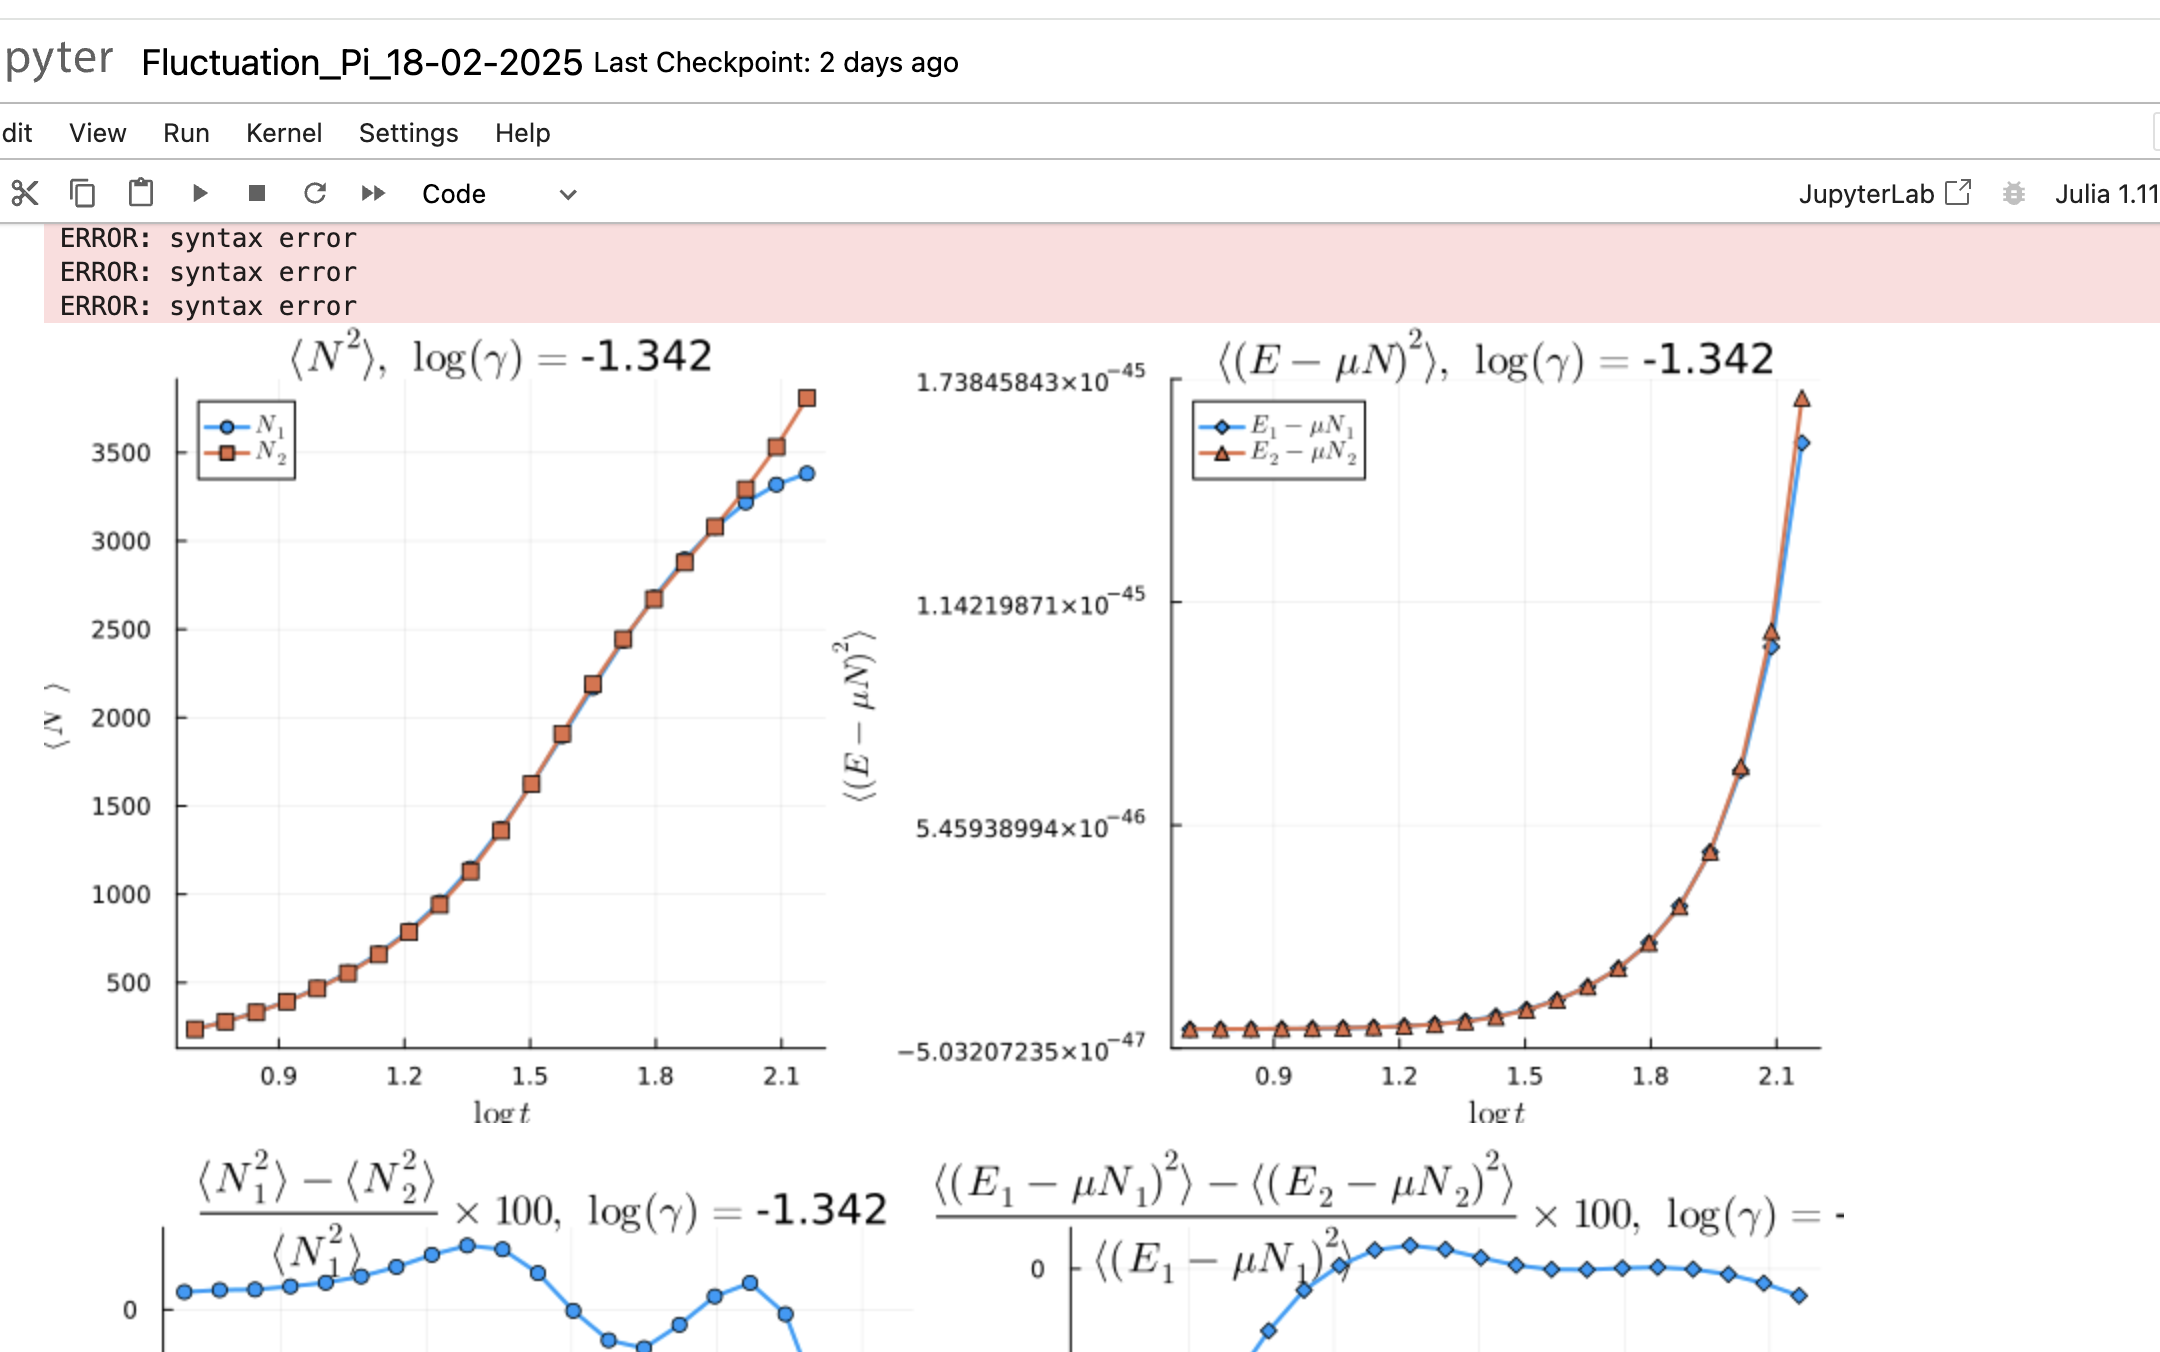
\includegraphics[width=1\textwidth]{Figures/test}

%\begin{aff}
%Donc une a l'ordre un en $\delta \theta (\operator{A}^{(0)})^{-1} %\operator{V}$ 

%\begin{eqnarray*}
%	\langle \delta \Pi ( \theta) \delta \Pi ( \theta') \rangle & = &  ( (\Pi^c_s - \Pi^c)\Pi^c/\Pi^c_s ) ( \theta ) \delta_{\theta, \theta'}/\delta \theta + \mathscr{F}(\theta , \theta' ) ,	
%\end{eqnarray*}

%avec 

%\begin{eqnarray*}
%	\mathscr{F}(\theta , \theta' ) & = & \left [ (\Pi^c_s - \Pi^c )( \theta)  +  (\Pi^c_s - \Pi^c ) ( \theta' )\right ] \frac{\Pi^c}{\Pi^c_s}(\theta)\frac{\Pi^c}{\Pi^c_s}(\theta') \frac{ \Delta( \theta'- \theta )}{ 2 \pi }\\
%	&&  - \left [ (\Pi^c_s - \Pi^c )( \theta)   (\Pi^c_s - \Pi^c ) ( \theta' )\right ] \frac{\Pi^c}{\Pi^c_s}(\theta)\frac{\Pi^c}{\Pi^c_s}(\theta')\int d\theta'' \left (   \frac{ \Pi^c/\Pi^c_s}{\Pi^c_s - \Pi^c} \right )(\theta'') \frac{\Delta(\theta''- \theta)}{2 \pi}\frac{\Delta(\theta''- \theta')}{2 \pi}  	
%\end{eqnarray*}
%\end{aff}



 








\subsection{Rôle des charges conservées extensives et quasi-locales}
%Dans les systèmes intégrables, l’état stationnaire atteint après une évolution hors d’équilibre n’est généralement pas décrit par un état de Gibbs classique, mais par un ensemble généralisé de Gibbs (GGE). Celui-ci est construit à partir de toutes les charges conservées du système

\paragraph{Écriture des observables thermodynamiques comme sommes sur les rapidités.}

%Dans le cas thermique, les valeurs moyennes des observables classiques telles que le nombre de particules et l'énergie peuvent s'exprimer comme des sommes de puissances des rapidités :
Dans un système à $N$ particules caractérisé par des rapidités ${ \theta_a }_{a = 1}^N$, les charges conservées classiques — telles que le nombre de particules, l’impulsion ou l’énergie — s’écrivent comme des sommes de puissances des rapidités :
\(
	\langle \operator{Q} \rangle_{\{ \theta_a\} } \propto \sum_{a = 1}^N \theta_a^0 , \,  \langle \operator{P} \rangle_{\{ \theta_a\} } \propto \sum_{a = 1}^N \theta_a^1  ,\,  \mbox{et} \langle \operator{H} \rangle_{\{ \theta_a\} } \propto \sum_{a = 1}^N \theta_a^2 .	
\)
(cf. équations \eqref{chap.2.gge.1})
Dans ce paragraphe précédent, nous avons sous-entendu — sans l’expliciter — qu’il est montré que l’ensemble des charges locales conservées forme une famille donnée par :
\begin{eqnarray}
	\operator{Q}_i^{(\mathcal{S})} \ket{\{\theta_a\} } & \propto & \sum_a \theta_a^i \ket{\{\theta_a\} }.
\end{eqnarray}
Ces charges agissent donc de manière diagonale sur les états de Bethe, avec des valeurs propres correspondant aux moments des rapidités.
%%%%%%%%%%%%%%%%%%%%%%%%%%%%%%%%%%%%%%%%%%%%%%%%%%
\paragraph{Charges conservées généralisées.\label{sec:charges-gen}}

%Les états propres du Hamiltonien de Lieb–Liniger~\eqref{eq:LL} sont les états de Bethe
%\(
%  \ket{\boldsymbol{\theta}}
%  =\ket{\theta_1,\dots,\theta_N}\!,
%\)
%déterminés par leurs rapidités \(\boldsymbol{\theta}\).
À toute fonction régulière
\(
  w:\mathbb R\!\to\!\mathbb R
\)
–– dorénavant appelée \emph{poids spectral}, ou \emph{énergie généralisée} ––
on associe un opérateur-charge généralisé :
\begin{eqnarray}\label{chap.2.charge.1}
	\operator{\mathcal{Q}}^{(\mathcal{S})}[w]\,\ket{\{\theta_a\} }&  = & \sum_{a=1}^{N}w(\theta_a)\,\ket{\{\theta_a\} } .	
\end{eqnarray}
Les choix particuliers
\(
  w(\theta)=1
\)
,
\(
  w(\theta)=\theta
\)
et
\(
  w(\theta)=\theta^{2}/2
\)
redonnent respectivement le nombre \(\operator{Q}=\operator{Q}_0^{(\mathcal{S})} = \operator{\mathcal{Q}}^{(\mathcal{S})}[1]\) , l’impulsion \(\operator{P}=\operator{Q}_1^{(\mathcal{S})} = \operator{\mathcal{Q}}^{(\mathcal{S})}[\theta]\) et l’Hamiltonien
\(\operator{H}=\operator{Q}_0^{(\mathcal{S})} = \operator{\mathcal{Q}}^{(\mathcal{S})}[\theta^2/2]\).

%Par construction toutes ces charges commutent,
%\(
%  [\hat Q[\omega_1],\hat Q[\omega_2]]=0,
%\)
%même si leur forme seconde‑quantifiée explicite n’est connue que pour quelques
%\(\omega\) simples.
Ces charges sont extensives : leur densité locale $\operator{q}^{(\mathcal{S})}[w]$ permet d’écrire
\(
  \operator{\mathcal{Q}}^{(\mathcal{S})}[w]=\int_0^{L}\!dx\;\operator{q}^{(\mathcal{S})}[w](x).
\)
%et la densité locale \(q[\omega](x)\) satisfait l’équation de continuité
%\[
%  \partial_t q[\omega](x)+\partial_x j[\omega](x)=0. \tag{31}
%\]

%Dans un état de Bethe \(\ket{\boldsymbol{\theta}}\) normalisé,
%la valeur moyenne exacte du courant vient de la formule récente de
%Borsi \textit{et al.}:
%\[
%  \frac{\langle\boldsymbol{\theta}|\,j[\omega](x)\,|\boldsymbol{\theta}\rangle}{L}
%  =\sum_{a,b=1}^{N}\omega'(\theta_a)\,[G^{-1}]_{ab}\,\theta_b, \tag{32}
%\]
%où \(G_{ab}=\partial p_a/\partial\theta_b\) est la matrice de Gaudin.
%%%%%%%%%%%%%%%%%%%%%%%%%%%%%%%%%%%%%%%%%%%%%%%%%%
%Dans le cas thermique, on peut remarquer que $\langle \operator{\mathcal{N}} \rangle_{\{ \theta_a\} } \propto \sum_{a = 1}^N \theta_a^0 $ et $\langle \operator{\mathcal{H}}_N \rangle_{\{ \theta_a\} } \propto \sum_{a = 1}^N \theta_a^2 $. On peut donc réécrire $\sum_{i = 1}^\infty  \beta_i \langle \operator{\mathcal{O}}_i \rangle_{ \{\theta_a \} }$

%Par analogie, la combinaison pondérée des valeurs moyennes d’un ensemble d’observables ${ \operator{\mathcal{O}}i }{i \in \mathbb{N}}$, associée aux multiplicateurs de Lagrange ${ \beta_i }$, peut être réécrite sous la forme :

%\begin{eqnarray}
%	\sum_{i = 1}^\infty  \beta_i \langle \operator{\mathcal{O}}_i \rangle_{ \{\theta_a \} } & = & \sum_{i = 0}^\infty \alpha_i \sum_{a = 1 }^N \theta_a^i		
%\end{eqnarray}
%où les coefficients $\alpha_i$ résultent d’une recombinaison des $\beta_i$.

%%%%%%%%%%%%%%%%%%%%%%%%%%%%%%%%%%%%%%%%%
%\paragraph{Interprétation fonctionnelle et échange des sommes.}
	
%Pour chaque $a \in \llbracket 1, N \rrbracket$, la série $\sum_i \alpha_i \theta_a^i$ converge pour des $\theta_a$ dans un domaine convenable, ce qui autorise l’échange de l’ordre des deux sommes : 
	
%\begin{eqnarray}
%	\sum_{i = 1}^\infty  \beta_i \langle \operator{\mathcal{O}}_i \rangle_{ \{\theta_a \} } & = & \sum_{a = 1 }^N  w(\theta_a) 
%\end{eqnarray}
	
%avec 
%\begin{eqnarray}
%	w(\theta) = \sum_{i=0}^\infty \alpha_i \theta^i.	
%\end{eqnarray}
%une fonction réelle (sous hypothèses de convergence). On peut ainsi réécrire la contribution totale des charges conservées comme une somme de termes mono-particulaires dépendant de la rapidité.
%La fonction $w(\theta)$ agit comme une fonction génératrice de poids associée aux charges conservées du système.

%%%%%%%%%%%%%%%%%%%%%%%%%%%%%%%%%%%%%%%%%
\paragraph{Expression de la matrice densité généralisée.}
La matrice densité généralisée s’écrit sous la forme :
\begin{eqnarray}\label{chap.2.densite.1}
	\operator{\rho}^{(\mathcal{S})}_{\mathrm{GGE}}[w]  =  \frac{e^{-\operator{\mathcal{Q}}^{(\mathcal{S})}[w]}}{Z^{(\mathcal{S})}[w]}, \, \mbox{avec} \quad e^{-\operator{\mathcal{Q}}^{(\mathcal{S})}[w]}  = 	\sum_{\{\theta_a \}} e^{- \sum_{a = 1}^N w(\theta_a) } \vert \{ \theta_a\} \rangle \langle  \{ \theta_a\}  \vert, 
\end{eqnarray}	
	%pour une certaine fonction $w$ relié à la charge% $\operator{\mathcal{Q}} [w]  = \sum_{\{\theta_a \}} \left ( \sum_{a = 1}^N w ( \theta_a )  \right ) \vert \{ \theta_a \} \rangle \langle \{ \theta_a \} \vert $.
%où l'opérateur de charge associé à $w$ s’écrit :
%\begin{eqnarray}
%	\operator{\mathcal{Q}} [w]   & = &  \sum_{\{\theta_a \}} \left ( \sum_{a = 1}^N w ( \theta_a )  \right ) \vert \{ \theta_a \} \rangle \langle \{ \theta_a \} \vert,	
%\end{eqnarray}
et la fonction de partition $Z^{(\mathcal{S})}[w]$ est définie par :
\(
	Z^{(\mathcal{S})}[w]   =  \sum_{\{\theta_a \}} e^{-\sum_{a = 1}^N w(\theta_a)}.		
\)

%%%%%%%%%%%%%%%%%%%%%%%%%%%%%%%%%%
\paragraph{Probabilité associée à une configuration de rapidités.}
	%Et on peut réecrire la probabilité de la configuration $\{\theta_a\}$ :% $ P_{\{ \theta_a \}} = \langle \{ \theta_a \}\vert \operator{\rho}_{GGE}[w] \vert  \{ \theta_a \} \rangle = e^{-\sum_{a = 1}^N w(\theta_a)} / Z $ avec $Z = \sum_{\{\theta_a \}} e^{-\sum_{a = 1}^N w(\theta_a)}$.\\
	%La probabilité d’occuper un état à $N$ particules caractérisé par les rapidités ${\theta_a}$ est alors :
La probabilité d’occuper l’état $\ket{\{\theta \}}$ est donc
\begin{eqnarray}
	\mathbb{P}^{(\mathcal{S})}_{\{ \theta_a \}} ~=~ \mathrm{Tr} \left [\operator{\rho}^{(\mathcal{S})}_{\mathrm{GGE}}[w] \vert \{ \theta_a \} \rangle \langle \{ \theta_a \} \vert  \right ] ~= ~ \langle \{ \theta_a \}\vert \operator{\rho}^{(\mathcal{S})}_{\mathrm{GGE}}[w] \vert  \{ \theta_a \} \rangle = Z^{(\mathcal{S})}[w]^{-1}e^{-\sum_{a = 1}^N w(\theta_a)}. 		
\end{eqnarray}
%Cela montre que le poids statistique d’une configuration factorise naturellement sur les pseudo-moments, avec un poids spectrale / energie génralisé $w(\theta)$ attribué à chaque particule.
On voit ainsi que le poids statistique factorise naturellement sur les
pseudo‑moments, chaque particule étant pondérée par $w(\theta_a)$.

%avec 
%\begin{eqnarray}
%	Z  & = & \sum_{\{\theta_a \}} e^{-\sum_{a = 1}^N w(\theta_a)}.		
%\end{eqnarray}


%%%%%%%%%%%%%%%%%%%%%%%%
\paragraph{Moyennes d'observables dans le GGE.}
%La valeur moyenne d’un observable locale $\operator{\mathcal{O}}$ dans l’ensemble généralisé s’écrit :
Pour tout opérateur local $\operator{\mathcal{O}}$ diagonal dans la base de Bethe,
la moyenne généralisée vaut
\begin{eqnarray}\label{chap.2.moyenne.1}
	\langle \operator{\mathcal{O}}\rangle_{GGE} & \doteq & \displaystyle  \text{Tr} (\operator{\mathcal{O}}\operator{\rho}^{(\mathcal{S})}_{\mathrm{GGE}}[w]) = \frac{\text{Tr} (\operator{\mathcal{O}}e^{-\operator{\mathcal{Q}}^{(\mathcal{S})}[w]})}{\text{Tr} (e^{-\operator{\mathcal{Q}}^{(\mathcal{S})}[w]})}	 = \frac{\sum_{\{\theta_a \}} \langle  \{ \theta_a\}  \vert   \operator{\mathcal{O}} \vert \{ \theta_a\} \rangle e^{- \sum_{a = 1}^N w(\theta_a) }  }{\sum_{\{\theta_a  \}} e^{- \sum_{a = 1}^N  w(\theta_a) } }
\end{eqnarray}
%Cette expression formelle montre que la connaissance de $w(\theta)$ suffit à déterminer les propriétés statistiques de toutes les observables diagonales dans cette base, incluant les charges conservées elles-mêmes.
Ainsi, la connaissance de la fonction $w(\theta)$ suffit à déterminer
les propriétés statistiques de toute observable diagonale,
y compris les charges conservées elles‑mêmes.	
	% Nous aimerions calculer les valeurs d'attente par rapport à cette matrice de densité, par exemple
	%La moyenne GGE d'un observable s'écrit ,
	%\begin{aff}
	%\begin{eqnarray}
	%	\langle \operator{\mathcal{O}} \rangle_{GGE} & \doteq & \displaystyle  \text{Tr} (\operator{\mathcal{O}}\operator{\rho}[w]) = \frac{\text{Tr} (\operator{\mathcal{O}}e^{-\operator{\mathcal{Q}}[w]})}{\text{Tr} (e^{-\operator{\mathcal{Q}}[w]})}	 = \frac{\sum_{\{\theta_a \}} \langle  \{ \theta_a\}  \vert   \operator{\mathcal{O}} \vert \{ \theta_a\} \rangle e^{- \sum_{a = 1}^N w(\theta_a) }  }{\sum_{\{\theta_a  \}} e^{- \sum_{a = 1}^N  f(\theta_a) } }
		%& =  & \frac{ \sum_{\pi} \sum_{\vert \{\theta_a \}\rangle \vert \Pi } \langle  \{ \theta_a\}  \vert   \operator{\mathcal{O}} \vert \{ \theta_a\} \rangle e^{- \sum_{a = 1}^N f(\theta_a) }  }{\sum_{\pi} \sum_{\vert \{\theta_a \}\rangle \vert \Pi }  e^{- \sum_{a = 1}^N  f(\theta_a) } }
	%\end{eqnarray}
	%pour une certaine observable $\operator{\mathcal{O}}$.\\
	%\end{aff}
	

\paragraph{Conclusion de la section : vers la thermodynamique de Bethe.}

Nous avons vu que, dans un système intégrable, la description correcte de l’équilibre stationnaire requiert l’introduction d’une \emph{famille infinie de charges conservées}, comprenant à la fois des charges strictement locales et des charges quasi‑locales.
Toutes ces charges se réunissent dans l’opérateur fonctionnel
\(
\operator{\mathcal{Q}}^{(\mathcal{S})}[w]
\)
, défini par un \emph{poids spectral}  $w(\theta)$ (cf. équations~\eqref{chap.2.charge.1}).
Cette construction conduit naturellement à la matrice densité généralisée
\(
\operator{\rho}^{(\mathcal{S})}_{\mathrm{GGE}}[w]  \propto  e^{-\operator{\mathcal{Q}}^{(\mathcal{S})}[w]}
\) 
(cf. équations~\eqref{chap.2.densite.1}), et à la moyenne d’un opérateur local $\operator{\mathcal{O}}$ donnée par
\(
\langle \operator{\mathcal{O}}\rangle_{GGE}  \doteq  \displaystyle  \text{Tr} (\operator{\mathcal{O}}\operator{\rho}^{(\mathcal{S})}_{\mathrm{GGE}}[w])
\)
(cf. équations~\eqref{chap.2.moyenne.1}).
La connaissance de $w(\theta)$ suffit donc pour prédire les valeurs moyennes de toutes les observables diagonales, y compris celles des charges elles‑mêmes ; c’est le cœur du {\bf Ensemble de Gibbs Généralisé (GGE pour Generalized Gibbs Ensemble)} .

\medskip
Cette base est désormais posée : dans la section suivante, nous passerons au \emph{thermodynamique de Bethe}.
Nous verrons comment, dans la limite thermodynamique, les sommes sur les configurations de rapidités se transforment en intégrales sur des densités continues, comment apparaît l’entropie de Yang–Yang, et comment les moyennes de l’ensemble généralisé se réexpriment à l’aide de ces densités macroscopiques.
C’est ce formalisme qui permettra d’analyser finement la relaxation post‑quench et de relier microscopie intégrable et hydrodynamique généralisée.



%%Dans ce chapitre, nous nous intéressons aux fluctuations de la distribution de rapidité \( \delta \rho \) autour d'une distribution de référence \( \rho^c \), qui maximise la contribution à la fonction de partition des états, exprimée comme une fonctionnelle de la distribution \( \rho \) : 

La fonction de partition des états, s'exprime comme une fonctionnelle de la distribution \( \rho \) : 

\begin{eqnarray*}
	\Xi & = & \sum_\rho \exp \left( -\mathcal{A}(\rho) \right).
\end{eqnarray*}  

Dans la section {\em \bf Entropie de Yang-Yang} (\ref{??}), l'action \( \mathcal{A}(\rho) \) s'écrit sous la forme :  

\begin{eqnarray*}
	\mathcal{A}(\rho) & \doteq & - L\mathcal{S}_{YY}(\rho) + L\int f(\theta) \rho (\theta) \, d\theta,		
\end{eqnarray*}  

où \( \mathcal{S}_{YY} \) est la fonctionnelle d'entropie de Yang-Yang, définie dans (\ref{??}), et \( f \) est la fonction paramétrant les charges, introduite dans (\ref{??}).  

Dans cette même section {\em \bf Entropie de Yang-Yang} (\ref{??}), nous avons établi un lien entre \( f \) et distribution de référence \( \rho^c \), qui maximise la contribution à la fonction de partition des états .\\

On veux tester si nos experience est décrit pas un GGE. Pour cela nous nous intéressons aux fluctuations de la distribution de rapidité \( \delta \rho \) autour \( \rho^c \).

%Nous poursuivons à présent avec cette définition de l'action de classe $\mathcal{C}^2$ et admetant une distribution critique $\rho^c$ tel que sa différentielle en ce point critique soit nulle $d\mathcal{A}_{\rho^c} = 0 $ (\ref{??}) de sorte que d'aprés la formule de Taylor-Youg %afin de déterminer les fluctuations autour de \( \Pi^c \). Pour cela, nous réécrivons l'action sous la forme :  

Nous poursuivons à présent avec cette définition de l'action de classe $\mathcal{C}^2$ et admetant une distribution critique $\rho^c$ tel que sa différentielle en ce point critique soit nulle $d\mathcal{A}_{\rho^c} = 0 $ (\ref{??}) de sorte que d'aprés la formule de Taylor-Youg %afin de déterminer les fluctuations autour de \( \Pi^c \). Pour cela, nous réécrivons l'action sous la forme :  

\begin{eqnarray*}  
	\mathcal{A}(\rho^c + \delta \rho) & \underset{ \delta \rho \to 0 }{=} & \mathcal{A}(\rho^c)  + \frac{1}{2} \left. \frac{\delta^2 \mathcal{A}}{\delta \rho^2} \right|_{\rho^c} (\delta \rho) + \mathcal{O}((\delta \rho)^3),  
\end{eqnarray*}  

une expression quadratique pour l'action à l'ordre dominant en \( \delta \Pi \) avec $\left. \frac{\delta^2 \mathcal{A}}{\delta \rho^2} \right|_{\rho^c}$ la forme quadratique définie positive (Fig (\ref{fig.fluctu.A})).

\begin{figure}[H]
	\centering 
	\begin{tikzpicture}
		\begin{scope}[shift={(0,0)}]
			\begin{scope}[transform canvas={scale=0.6}]
				% Définition des couleurs avec les codes HTML
\definecolor{colorOne}{HTML}{443E46}
\definecolor{colorTwo}{HTML}{F6DEB8}
\definecolor{colorThree}{HTML}{908CA4}
\definecolor{colorFour}{HTML}{57659E}
\definecolor{colorFive}{HTML}{C57284}
\definecolor{colorSix}{HTML}{FF5B69}

% Raccourcis pour les couleurs
\def\colorOne{colorOne}
\def\colorTwo{colorTwo}
\def\colorThree{colorThree}
\def\colorFour{colorFour}
\def\colorFive{colorFive}
\def\colorSix{colorSix}

\def\colorslide{blue!50!black}



\begin{scope}
	% Tracer une courbe lisse entre des points
	\draw[shift={(0,0)} ,\colorOne]
		(-1 , 0 ) edge [thick,line width=0.8ex , ->,>=triangle 45  , \colorOne] node [pos = 1 , below ]{\huge$\rho$}( 5  , 0 )
	;
	\draw[shift={(0,0)}, color=\colorOne]
		(0, -1.0 ) edge [thick,line width=0.8ex , ->,>=triangle 45  ]node [pos=0.9,left=0.2cm ]{\huge$\mathcal{A}(\rho)$}( 0  , 5 )
	;
	\draw[]
		(2.5, 0.12 ) edge [thick,line width=0.8ex ,\colorThree ]node [pos=1,below  ]{\huge$\rho^c$} (2.5, -0.12 )	
	;
	
	\draw[]
		(2.5, -0.12 ) edge [thick,line width=0.4ex , dashed, \colorThree ] (2.5, 5.5 )
		(1.5, 1 ) edge [thick,line width=0.4ex , <->,>=triangle 45  , \colorThree ] (3.5, 1 )
		(-0.3,1) edge [thick,line width=0.4ex  , \colorThree ] node [pos=0,left ]{\huge$\mathcal{A}(\rho^c)$} (0.3, 1 )	
	;
    \draw[thick, line width=0.8ex , \colorFour] plot[smooth, tension=0.7] coordinates {
        (1, 5) (1.6 , 3 ) (2.5, 1) (3.5 , 3 )  (4, 5)
    };		
	
\end{scope}

	
			
			\end{scope}
			
			\draw[color = red , scale = 0.5 , draw = none  ] (-2 , -1) rectangle (5, 6) ; 	
		\end{scope}
		
		\begin{scope}[shift={(19,-1)}]
			\begin{scope}[transform canvas={scale=0.6}]
				% Définition des couleurs avec les codes HTML
\definecolor{colorOne}{HTML}{443E46}
\definecolor{colorTwo}{HTML}{F6DEB8}
\definecolor{colorThree}{HTML}{908CA4}
\definecolor{colorFour}{HTML}{57659E}
\definecolor{colorFive}{HTML}{C57284}
\definecolor{colorSix}{HTML}{FF5B69}

% Raccourcis pour les couleurs
\def\colorOne{colorOne}
\def\colorTwo{colorTwo}
\def\colorThree{colorThree}
\def\colorFour{colorFour}
\def\colorFive{colorFive}
\def\colorSix{colorSix}

\def\colorslide{blue!50!black}

\def\Occupation{
	\def\traitx{0.3}
	\def\traity{0.5}
	\draw[shift={(0,0)}]
		(-13.5 , 0 ) edge [thick,line width=0.8ex ]( -3.2  , 0 )
		( -3.2 - \traitx  , 0 - \traity ) edge [thick,line width=0.8ex ]( -3.2 + \traitx  , 0 + \traity  )
		( -2.8 - \traitx  , 0 - \traity ) edge [thick,line width=0.8ex ]( -2.8 + \traitx  , 0 + \traity  )
		(-2.8 , 0 ) edge [thick,line width=0.8ex ](2.8  , 0 )
		( 2.8 - \traitx  , 0 - \traity ) edge [thick,line width=0.8ex ]( 2.8 + \traitx  , 0 + \traity  )
		( 3.2 - \traitx  , 0 - \traity ) edge [thick,line width=0.8ex ]( 3.2 + \traitx  , 0 + \traity  )
		(3.2, 0 ) edge [thick,line width=0.8ex,->,>=triangle 45 , color = black ]node [pos=1.01,below  ]{\huge$\theta$}	( 13  , 0 )
	;
	\draw[shift={(0,0)}, color=\colorOne]
		(-10.5 , -1.5 ) edge [thick,line width=0.8ex , ->,>=triangle 45  ]( -10.5  , 4.5 )
	;
		
	\foreach \r in {1 , ... , 3 } {
%		\draw[
%		decoration={
%		markings,
%    	mark connection node=my node,
%    	mark=at position 0 with{\node [blue,transform shape] (my node) {\large \r};}},
%		color=gray, thick, 
%		line width=0.5ex] decorate { 
%            (-11.0, \r) -- (-10.1, \r )}
%        ;
        \draw[
			color=\colorOne,
			] 
            (-11.0, \r) edge[color=\colorThree , thick,line width=0.5ex] node [pos=-0.5 ]{\large\color{\colorFour} $\frac{\r}{\delta \theta}$ } (-10.3, \r )
        	;
	
	}
	

	
	% Graduation abcsisse 
	% Définitions des listes
% Definitions of the lists
\def\listetuple{-9/\theta_{1}, -8/\theta_{2} , -5/\theta_{3} , -2/\theta_{a-1} , 0/\theta_{a} , 1/\theta_{a+1} , 2/\theta_{a+2} ,  5/\theta_{N-4} , 7/\theta_{N-3},8/\theta_{N-1},9/\theta_{N} }
\def\listetrais{-12 , -11, -10, -9 , -8 , -7 ,  -6 , -5, -4.5,-4, -2 , -1, 0 , 0.5, 1, 2, 4 , 5 ,  6 , 7 , 8 ,8.5, 9 ,  10 , 11, 12 }

% Loop over listetrais
\foreach \r in \listetrais {
    % Initialize found variable to zero
    % Initialize found variable to zero
    %\pgfmathsetmacro\found{0}
    \global\def\found{0}
    \xdef\nomtheta{}
    
    % Check if \r is in listetuple
    \foreach \x/\y in \listetuple { 
        \ifdim \r pt=\x pt % If \r matches any \x in listetuple
            \global\def\found{1} ;
            \xdef\nomtheta{\y} % Set \nomtheta to the corresponding \y
            %\pgfmathsetmacro\found{1} % Set found to 1            
            %\global\pgfmathsetmacro\found{1}
        \fi
    }
    
    %\node [circle, draw, red] (A) at (\r, 2) {\found , $\nomtheta$};
    
    % Draw the line and display \nomtheta if found
    \ifnum\found=1
        \draw[color=\colorOne, thick, line width=0.5ex] 
            (\r, -0.3) -- (\r, 0.3) node[red , pos=-0.5] {\large $\nomtheta$};
         \filldraw[line width=0.5ex, color=\colorSix, outer color=\colorSix, inner color=\colorSix] 
            (\r, 0) circle (4pt);
    \else 
        % Draw without \nomtheta and add a blue circle if not found
        \draw[color=\colorOne, thick, line width=0.5ex] 
            (\r, -0.3) -- (\r, 0.3);
        \filldraw[line width=0.5ex, color=\colorSix, outer color=\colorTwo, inner color=\colorTwo] 
            (\r, 0) circle (4pt); 
    \fi
}

\def\listetrais{-9.5/\theta_{i-1}/2/3, -6.5/\theta_{i}/1/4  ,   -1.5/\theta_{j}/2/4 , 1.5/\theta_{j+1}/-1/3 , 3.5/\theta_{\ell-1}/1/3 , 6.5/\theta_{\ell}/3/4 , 9.5/\theta(\theta_{\ell+1})/-1/3 };



\foreach \r/\nomx/\y/\ys in \listetrais {
	\draw[
		decoration={
		markings,
    	mark connection node=my node,
    	mark=at position .5 with{\node [blue,transform shape] (my node) {\large \color{\colorFour} $\nomx$};}},
		color=\colorThree , thick, 
		line width=0.5ex] decorate { 
            (\r, 0.12) -- (\r, -1.2)}
        ;
     
     \ifdim \y pt > -1 pt 
     	\draw[
			decoration={
			markings,
    		mark connection node=my node,
    		mark=at position .5 with{\node [blue,transform shape] (my node) {\large \color{\colorFour} $\Pi(\nomx) $};}},
			color=\colorThree, thick, 
			line width=0.5ex] decorate { 
            (\r, \y) -- (\r +3, \y)}
        ;
        \draw[
			decoration={
			markings,
    		mark connection node=my node,
    		mark=at position .5 with{\node [blue,transform shape] (my node) {\large \color{\colorFive} $\Pi_s(\nomx) $};}},
			color=\colorFive, thick, 
			line width=0.5ex] decorate { 
            (\r, \ys) -- (\r +3, \ys)}
        ;
     \fi 
     \ifdim \r pt= -1.5 pt
     	\draw[
     		decoration={
			markings,
    		mark connection node=my node,
    		mark=at position .5 with{\node [blue,transform shape] (my node) {\large \color{\colorFour}  $\delta \theta $};},
    		%mark=at position 0.1  with {\arrow[blue, line width=0.5ex]{<}},
    		%mark=at position 1  with {\arrow[blue, line width=0.5ex]{>}}
    		},
        	color=\colorThree,
        	thick,
        	line width=0.5ex,
        	%arrows={Computer Modern Rightarrow[line cap=round]-Computer Modern Rightarrow[line cap=round]}
   			](\r, -1.2) edge[arrows={Computer Modern Rightarrow[line cap=round]-}] (\r + 0.4, -1.2)decorate {
    		(\r, -1.2) -- (\r + 3, -1.2)}(\r + 2, -1.2) edge[arrows={-Computer Modern Rightarrow[line cap=round]}] (\r + 3, -1.2)
    		;
    \fi
			
	
}


			
}


\begin{scope}
	%\draw[help lines , width=1.5ex] (-8,-3) grid (8,3);\draw[help lines ,width=0.5ex , opacity = 0.5] (-3,-3) grid[step=0.1] (3,3));
	
	%\draw[help lines] 
	%	(-3,-3) edge[width=1.5ex] grid (3,3)	
	%	(-3,-3) edge[width=0.5ex , opacity = 0.5] grid (3,3)	
	%;
	\begin{scope}[shift={(0,1)},rotate=0,opacity=1,color=black]
		\Occupation	
		
		%\node[anchor=east, font=\bfseries] at (-11, 0) {\color{red}\large (T = 0 )} ;	
	\end{scope}
	
	
	
	
	\begin{scope}[shift={(-10.5,7)},rotate=0,opacity=1,color=black]
	
	\begin{scope}[shift={(-0,0)},rotate=0,opacity=1,color=black]
	
		\draw[shift={(0,0)} ,line width=1ex,rounded corners = 1ex,color=\colorOne , opacity =1 ,fill=\colorOne!00 , pattern={north east lines} , pattern color=\colorOne!00 ]
			(0 , -1 ) rectangle (5,1)
		;
		

		\begin{scope}[shift={(0.5,0.5)}]
			\draw[color=\colorOne, thick, line width=0.5ex] 
            (0, -0.3) -- (0, 0.3) ;
            \filldraw[line width=0.5ex, color=\colorSix, outer color=\colorSix, inner color=\colorSix] 
            (0, 0) circle (4pt);
            
            \node[anchor=west, font=\bfseries] at (0.2, 0) {\color{\colorSix}\large : quasi-particule};
		\end{scope}
		
		\begin{scope}[shift={(0.5,-0.5)}]
			\draw[color=\colorOne, thick, line width=0.5ex] 
            (0, -0.3) -- (0, 0.3) ;
            \filldraw[line width=0.5ex, color=\colorSix, outer color=\colorTwo, inner color=\colorTwo] 
            (0, 0) circle (4pt);
            
            \node[anchor=west, font=\bfseries] at (0.2, 0) {\color{\colorSix}\large : hole};
		\end{scope}

	\end{scope}
	
	\begin{scope}[shift={(6,0)},rotate=0,opacity=1,color=black]	
		
		\draw[shift={(0,0)} ,line width=1ex,rounded corners = 1ex,color=\colorOne , opacity =1 ,fill=\colorOne!00 , pattern={north east lines} , pattern color=\colorOne!00 ]
			(0 , -1 ) rectangle (7.5,1)
		;
		
		\node[anchor=west] at (0.5, 0.5) {\color{\colorFour}\large $\Pi$ };\node[anchor=west, font=\bfseries] at (1, 0.5) {\color{\colorFour}\large : quasi-particule distribution};
		
		\node[anchor=west] at (0.5, -0.5) {\color{\colorFour}\large $\Pi_h$ };\node[anchor=west, font=\bfseries] at (1, -0.5) {\color{\colorFour}\large  : hole distribution};
		
	\end{scope}
	
	\begin{scope}[shift={(14.5,0)},rotate=0,opacity=1,color=black]	
		
		\draw[shift={(0,0)} ,line width=1ex,rounded corners = 1ex,color=\colorOne , opacity =1 ,fill=\colorOne!00 , pattern={north east lines} , pattern color=\colorOne!00 ]
			(0 , -0.5 ) rectangle (7.0,0.5)
		;
		
		\node[anchor=west] at (0.2, 0) {\color{\colorFour}\large ${\color{\colorFive}\Pi_s} = \Pi + \Pi_h $ } node[anchor=west , font=\bfseries] at (3.1 , 0 )  {\color{\colorFour}\large {\color{\colorFive} : density of states}};
		
	\end{scope}
	
	
	\end{scope}


		
	
\end{scope}

	
			
			\end{scope}
			\begin{scope}[scale=1]
				\draw[color = red , scale = 1 , draw = none  ] (-1 , -1) rectangle (5, 5) ; 
			\end{scope}	
		\end{scope}

		
				
			
	\end{tikzpicture}	
	\captionsetup{skip=10pt} % Ajoute de l’espace après la légende
	\label{fig.fluctu.A}
\end{figure}


On discrétise l'axe des rapidités en  petite cellule de rapidité $[\theta, \theta+\delta\theta]$, qui contient $L\rho(\theta) \delta \theta$ rapidités. 
	



Avec ces petites tranches, la forme quadratique s’écrit :

\begin{eqnarray*}
    \left. \frac{\delta^2 \mathcal{A}}{{\delta \rho}^2} \right|_{\rho^c}(\delta \rho ) &=&  \sum_{a,b \mid \text{tranche}}  
    \delta \rho(\theta_a)  \frac{\partial^2 \mathcal{A}}{\partial \delta \rho(\theta_a) \partial \delta \rho(\theta_b) } (\rho^c)  \delta \rho(\theta_b).
\end{eqnarray*}
Les fluctuations s’écrivent donc :

\begin{eqnarray*}
    \langle \delta \rho ( \theta) \delta \rho ( \theta') \rangle &=&  
    \frac{ \int d\delta \rho \, \delta \rho(\theta) \delta \rho ( \theta') 
    \exp \left( - \frac{1}{2} \sum_{a,b \mid \text{tranche}}  
    \delta \rho(\theta_a) \frac{\partial^2 \mathcal{A}}{\partial \delta \rho(\theta_a) \partial \delta \rho(\theta_b) } (\rho^c)  \delta \rho(\theta_b) \right) }
    { \int d\delta \Pi  
    \exp \left( - \frac{1}{2} \sum_{a,b \mid \text{tranche}}  
    \delta \rho(\theta_a) \frac{\partial^2 \mathcal{A}}{\partial \delta \rho(\theta_a) \partial \delta \rho(\theta_b) } (\rho^c)  \delta \rho(\theta_b) \right) } \\
    &=& \left( \mathbf{A}^{-1} \right)_{\theta , \theta'}
\end{eqnarray*}


\begin{aff}

\begin{eqnarray*}
	\langle \delta \rho ( \theta) \delta \rho ( \theta') \rangle &=& 	\left( \mathbf{A}^{-1} \right)_{\theta , \theta'}
\end{eqnarray*}

	
avec la  {\em matrice hessienne} $\mathbf{A}_{\theta , \theta'} \equiv \frac{\partial^2 \mathcal{A}}{\partial \delta \rho(\theta) \partial \delta \rho(\theta') }(\rho^c)$, au point critique/ qui maximise la probabilité  $\rho^c=\rho^c_s \nu^c $, s'écrit

\begin{eqnarray*}
	\operator{A} & = & \operator{A}^{(0)} + \delta \theta \operator{V}
\end{eqnarray*}

avec 

\begin{eqnarray*}
	A^{(0)}_{\theta , \theta'}  & = &  L\delta \theta \left ( \frac{ 1}{\rho^c_s ( 1  - \nu^c ) \nu^c } \right )(\theta)    \delta({\theta - \theta '})	,\\
	V_{\theta , \theta'}  &= & L \delta \theta \left \{ - \left [ \left ( \frac{1}{\rho^c_s( 1 - \nu^c) } \right ) ( \theta)  +  \left ( \frac{1}{\rho^c_s( 1 - \nu^c) } \right ) ( \theta' )\right ] \frac{ \Delta( \theta'- \theta )}{ 2 \pi } + \int d\theta''  \left ( \frac{\nu^c}{\rho^c_s( 1 - \nu^c) } \right )(\theta'') \frac{\Delta(\theta''- \theta)}{2 \pi}\frac{\Delta(\theta''- \theta')}{2 \pi}   \right \} 	
\end{eqnarray*}

\end{aff}

\subsection{Testes}

\begin{eqnarray*}
	\Delta_{\operator{\mathcal{N}}}^2  & = &  \frac{1}{\beta} \left . \frac{\partial \langle \operator{\mathcal{N}} \rangle}{\partial \mu} \right )_T \\
	\Delta_{\operator{\mathcal{E}}-\mu \operator{\mathcal{N}}}^2  & = &  - \left . \frac{\partial \langle \operator{\mathcal{E}}-\mu \operator{\mathcal{N}} \rangle}{\partial \beta} \right )_\mu 
\end{eqnarray*}

et 

\begin{eqnarray*}
	\Delta_{\operator{\mathcal{N}}}^2  &= & L^2 \int d\theta_a \int d \theta_b \, \langle \delta \rho(\theta_a) \delta \rho(\theta_b) \rangle \\
	\Delta_{\operator{\mathcal{E}}-\mu \operator{\mathcal{N}}}^2  & = & L^2 \int d\theta_a \int d \theta_b \, \left ( - \mu + \frac{1}2 m \theta_a^2  \right  )\left ( - \mu + \frac{1}2 m \theta_b^2  \right  )  \langle \delta \rho(\theta_a) \delta \rho(\theta_b) \rangle
\end{eqnarray*}

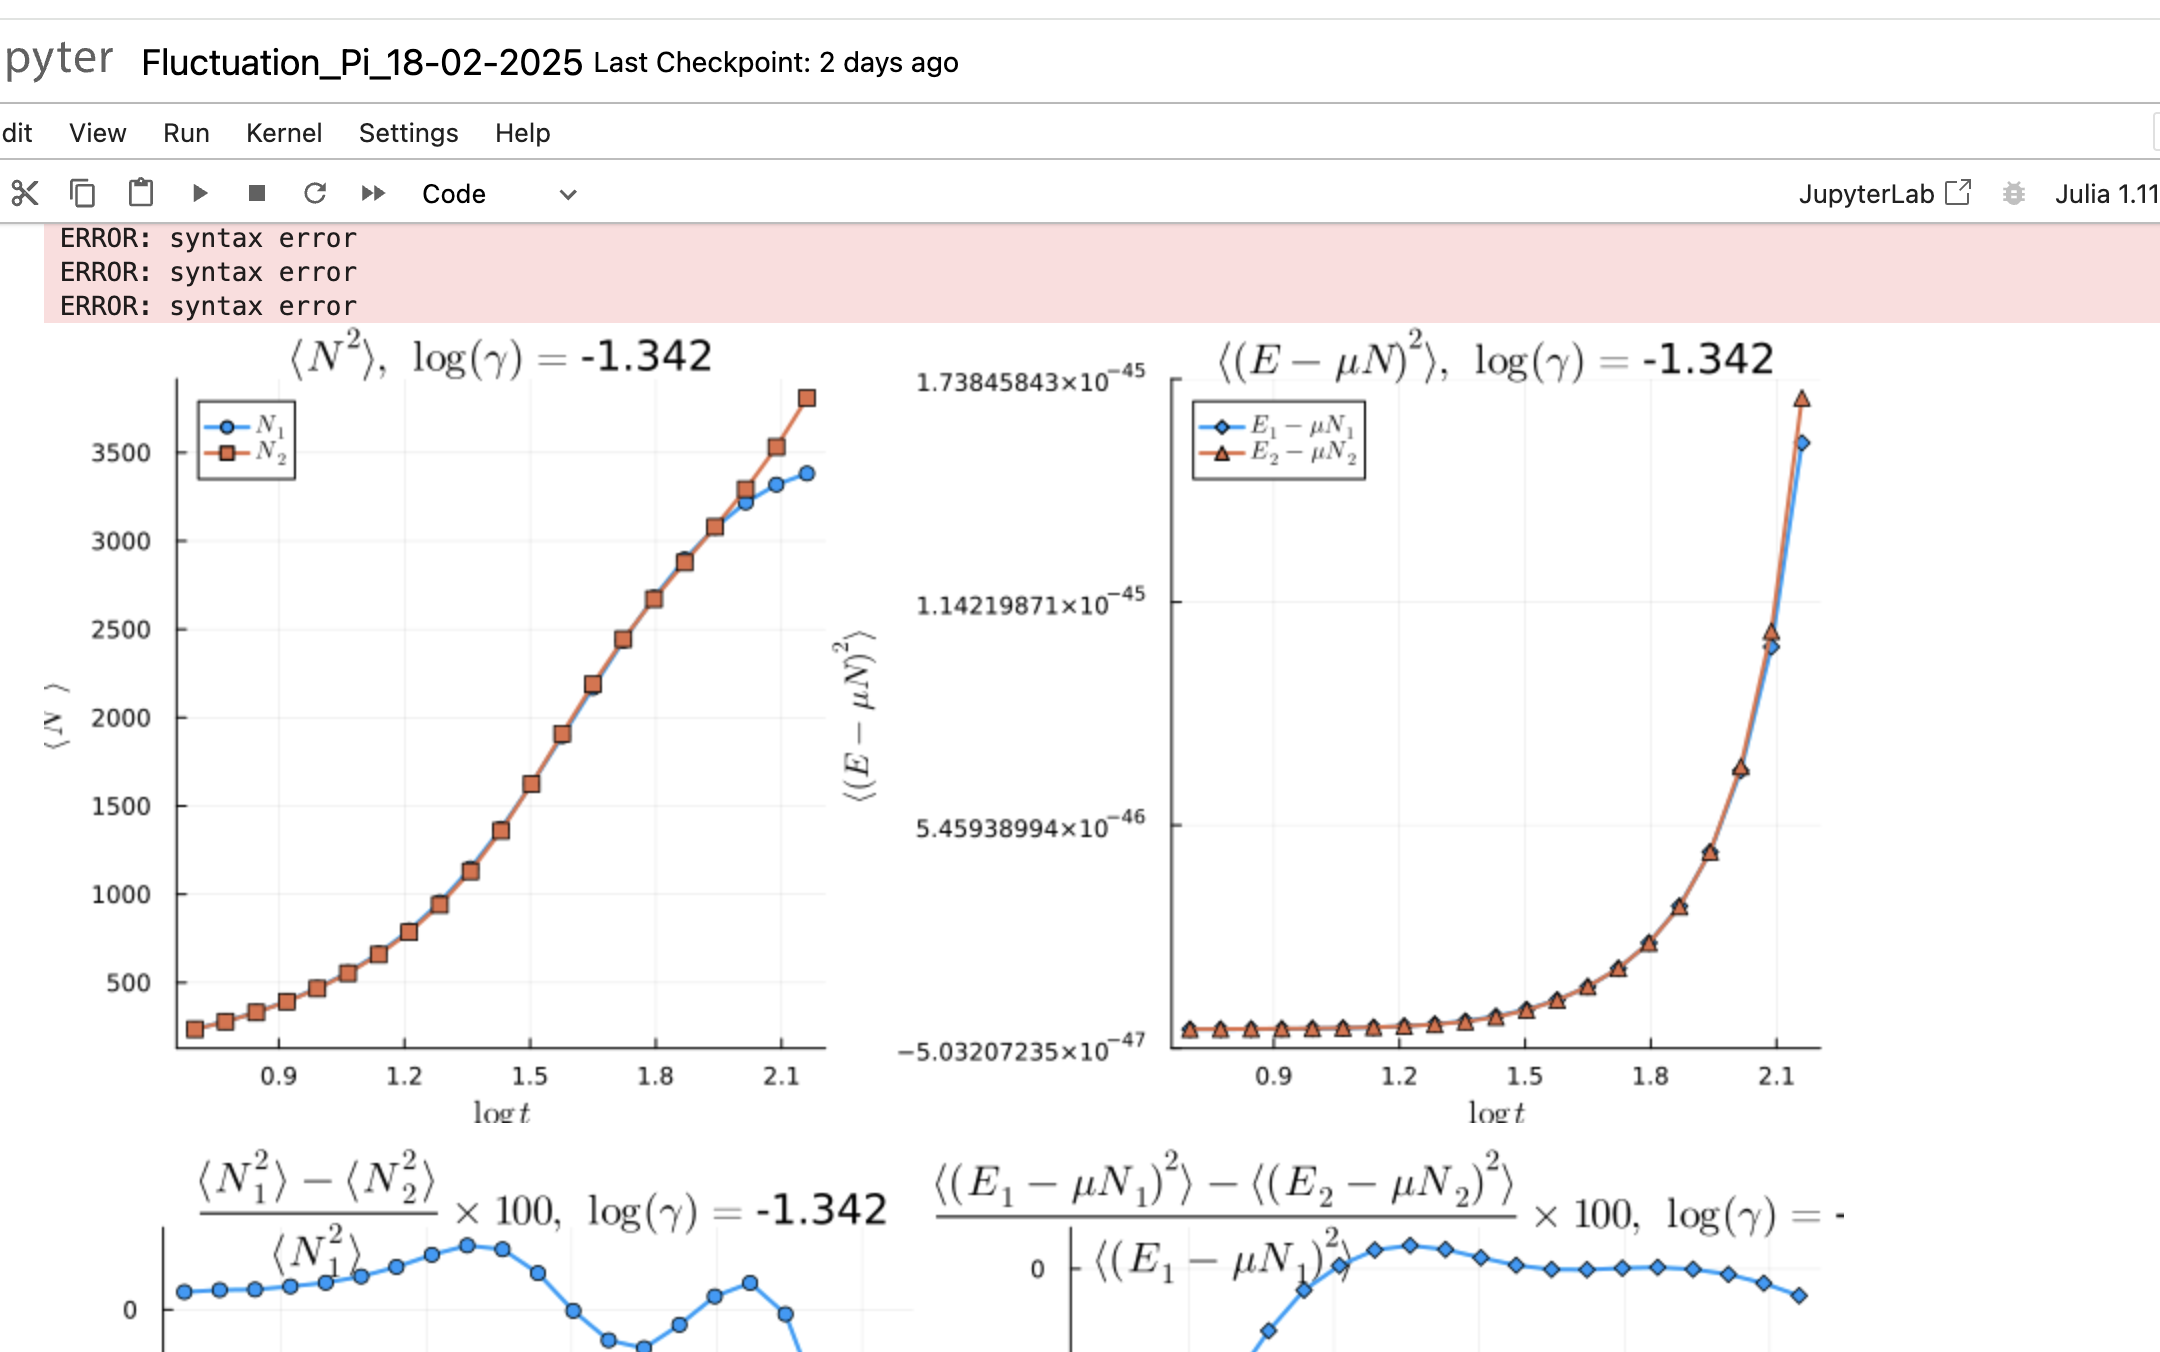
\includegraphics[width=1\textwidth]{Figures/test}

%\begin{aff}
%Donc une a l'ordre un en $\delta \theta (\operator{A}^{(0)})^{-1} %\operator{V}$ 

%\begin{eqnarray*}
%	\langle \delta \Pi ( \theta) \delta \Pi ( \theta') \rangle & = &  ( (\Pi^c_s - \Pi^c)\Pi^c/\Pi^c_s ) ( \theta ) \delta_{\theta, \theta'}/\delta \theta + \mathscr{F}(\theta , \theta' ) ,	
%\end{eqnarray*}

%avec 

%\begin{eqnarray*}
%	\mathscr{F}(\theta , \theta' ) & = & \left [ (\Pi^c_s - \Pi^c )( \theta)  +  (\Pi^c_s - \Pi^c ) ( \theta' )\right ] \frac{\Pi^c}{\Pi^c_s}(\theta)\frac{\Pi^c}{\Pi^c_s}(\theta') \frac{ \Delta( \theta'- \theta )}{ 2 \pi }\\
%	&&  - \left [ (\Pi^c_s - \Pi^c )( \theta)   (\Pi^c_s - \Pi^c ) ( \theta' )\right ] \frac{\Pi^c}{\Pi^c_s}(\theta)\frac{\Pi^c}{\Pi^c_s}(\theta')\int d\theta'' \left (   \frac{ \Pi^c/\Pi^c_s}{\Pi^c_s - \Pi^c} \right )(\theta'') \frac{\Delta(\theta''- \theta)}{2 \pi}\frac{\Delta(\theta''- \theta')}{2 \pi}  	
%\end{eqnarray*}
%\end{aff}



 









\section{Thermodynamique de Bethe et relaxation}

%------------------------------------------------------------------
\subsection{Limite thermodynamique}

\paragraph{Observables locales dans la limite thermodynamique.}
%Lorsque l'observable $\operator{\mathcal{O}}$ est suffisamment local, on croit que la valeur d'attente $\langle  \{ \theta_a\}  \vert   \mathcal{O} \vert \{ \theta_a\} \rangle$ ne dépend pas de l'état microscopique spécifique du système, de sorte qu'elle devient une fonctionnelle de $\Pi$ dans la limite thermodynamique.
Si l’observable $\mathcal{O}$ est suffisamment locale, sa valeur d’attente dans un état propre ne dépend pas des détails microscopiques, mais uniquement de la distribution de rapidité. On écrit alors :
\begin{eqnarray}
	\underset{\mbox{\tiny therm.}}{\lim} \langle  \{ \theta_a\}  \vert   \operator{\mathcal{O}} \vert \{ \theta_a\} \rangle & = & \langle \operator{\mathcal{O}}\rangle_{[\rho]},
\end{eqnarray}
où $\underset{\mbox{\tiny therm.}}{\lim}$ est la limite thermodinamique ($N,L \to \infty$ avec $N/L \to $ const).\\

\medskip
Dans un ensemble général (GGE), la valeur moyenne de l’observable \eqref{chap.2.moyenne.1} devient alors :	
	
\begin{eqnarray}\label{chap.2.moyenne.2}
	\underset{\mbox{\tiny therm.}}{\lim} \langle \operator{\mathcal{O}} \rangle_{GGE} & =  & \frac{  \displaystyle \sum_{\rho }  \langle \operator{\mathcal{O}}\rangle_{[\rho]} \Omega[\rho] e^{- \sum_{a = 1}^N  w(\theta_a)    }}{ \displaystyle \sum_{\rho }   \Omega[\rho]\,e^{- \sum_{a = 1}^N  w(\theta_a) } } ,
\end{eqnarray}
où $\Omega[\rho]$ désigne le nombre de micro-états compatibles avec la distribution de rapidité $\rho$.
%où $\# \mbox{micro-états.}$ est les nombre de micro état associée àa la distribution de rapidité $\rho$.
%Avant de se plonger sur $\# \mbox{micro-états.}$, regardons le changement des équation de Bethes. 

\medskip
Avant d’étudier la fonction $\Omega[\rho]$, examinons d’abord la transformation des équations de Bethe dans cette limite.


\paragraph{Équation de Bethe continue.}

À température non nulle (hors de l’état fondamental), il n’y a plus de mer de Fermi définie, et les équations \eqref{chap.1.rho.2} et \eqref{chap.1.rho.3} ne sont plus valides (en particulier $\rho \neq \rho_s$). Les équations discrètes de Bethe \eqref{chap.1.rho.s.2} se condensent alors en une équation intégrale pour les densités de rapidité :
\
\begin{equation}
	2\pi \rho_s \;=\; 1 \;+\;\Delta \star \rho,
\label{eq:TBA-rhos}
\end{equation}
où le symbole $\star$ désigne la \emph{convolution} :
\(
	[\Delta \star \rho](\theta) = \int_{-\infty}^{\infty} d\theta' \, \Delta(\theta - \theta') \, \rho(\theta').
\)
%Pour le modèle de \textbf{Lieb–Liniger} de couplage $g>0$.  
%le noyau
%\(
%\Delta(\theta)=\dfrac{2g}{\theta^{2}+g^{2}}
%\)
%provient de la dérivée de la phase de diffusion
%$S(\theta)=\dfrac{\theta-ic}{\theta+ic}$.

%------------------------------------------------------------------
%\subsection{Opération de \emph{dressing}}
%\label{sec:dressing}

%\subsubsection{Définition}

%\begin{align}
%f^{\mathrm{dr}}(\theta) &= f(\theta) \;+\;
%       \int_{-\infty}^{\infty}\!\frac{d\theta'}{2\pi}\;
%             \Delta(\theta-\theta')\,\nu(\theta')\,f^{\mathrm{dr}}(\theta')
%\nonumber\\
%&= f(\theta)\;+\;\Bigl[\tfrac{\Delta}{2\pi}\star\bigl(\nu\,f^{\mathrm{dr}}\bigr)
%     \Bigr](\theta),
%\label{eq:dressing}
%\end{align}

\paragraph{Opération de \emph{dressing}.}
\subparagraph{Définition.}
À toute fonction $f(\theta)$ on associe sa version \emph{habillée} (ou \emph{dressed}) $f^{\mathrm{dr}}(\theta)$, définie comme la solution de l’équation intégrale suivante :
\begin{eqnarray}
	f^{\mathrm{dr}} & = & f  \;+\;\Bigl[\tfrac{\Delta}{2\pi}\star\bigl(\nu\,f^{\mathrm{dr}}\bigr)\Bigr] \label{eq:dressing}	
\end{eqnarray}
où $\nu = \rho/\rho_s$ est le \emph{facteur d’occupation}, et $\Delta/2\pi$ est le noyau de diffusion du modèle.

%où $\Delta/2\pi$ est un noyau de convolution spécifique et 
%\(
%\nu=\dfrac{\rho}{\rho_s}
%\)
%est le \emph{facteur d’occupation}.

\subparagraph{Interprétation physique}

Le dressing incorpore à tous ordres les effets de rétrodiffusion entre quasi-particules. Il encode ainsi les corrections d’interaction aux grandeurs physiques initiales $f(\theta)$. Dans le modèle de Lieb–Liniger, cette opération permet de déterminer : l’énergie habillée $\varepsilon^{\mathrm{dr}}(\theta)$ , l’impulsion habillée $p^{\mathrm{dr}}(\theta)$ , les susceptibilités thermodynamiques (cf. section~\ref{chap:GGE}).

{\color{blue}
\paragraph{Susceptibilités thermodynamiques.}

Les susceptibilités thermodynamiques décrivent la réponse linéaire du système à une variation infinitésimale de paramètres thermodynamiques conjugués aux charges conservées. Pour un système intégrable, elles mesurent la sensibilité des valeurs moyennes $\langle Q_i \rangle$ des charges conservées $Q_i$ par rapport aux potentiels thermodynamiques $\mu_j$ associés à ces charges :

\begin{equation}
    \chi_{ij} = \frac{\partial \langle Q_i \rangle}{\partial \mu_j}.
\end{equation}

Dans le cadre de la thermodynamique de Bethe, ces susceptibilités s’expriment à l’aide des fonctions habillées. Si $q_i(\theta)$ est la densité de charge $Q_i$ portée par une quasi-particule de rapidité $\theta$, alors la densité totale de charge est donnée par :

\begin{equation}
    \langle Q_i \rangle = \int d\theta\, \rho(\theta)\, q_i^{\mathrm{dr}}(\theta),
\end{equation}

où $q_i^{\mathrm{dr}}(\theta)$ est la charge habillée, solution de l’équation de dressing :

\begin{equation}
    q_i^{\mathrm{dr}}(\theta) = q_i(\theta) + \int \frac{d\theta'}{2\pi}\, \Delta(\theta - \theta')\, \nu(\theta')\, q_i^{\mathrm{dr}}(\theta').
\end{equation}

Par différentiation par rapport aux $\mu_j$, on obtient :

\begin{equation}
    \chi_{ij} = \int d\theta\, \rho_s(\theta)\, \nu(\theta)\, q_i^{\mathrm{dr}}(\theta)\, q_j^{\mathrm{dr}}(\theta),
\end{equation}

où $\rho_s(\theta)$ est la densité de sites disponibles, $\nu(\theta) = \rho(\theta)/\rho_s(\theta)$ est le facteur d’occupation, et $\Delta(\theta)$ est le noyau issu de la phase de diffusion du modèle considéré.

Ces susceptibilités interviennent dans la théorie hydrodynamique généralisée (GHD) comme coefficients de la métrique thermodynamique et des corrélations à longue distance. Elles permettent également d’exprimer les fluctuations thermiques et les coefficients de transport linéaire (formules de Kubo généralisées).

%\begin{tcolorbox}[colback=gray!5,colframe=gray!40!black,title=Exemple : susceptibilités dans le modèle de Lieb–Liniger]
\begin{mdframed}[
	linewidth=0.5pt, 
	backgroundcolor=gray!5, 
	roundcorner=50pt,	
	innerleftmargin=5pt,
    innerrightmargin=5pt,
    innertopmargin=5pt,
    innerbottommargin=2pt,
    leftmargin=2pt,
    rightmargin=2pt
	]
	

Dans le modèle de Lieb–Liniger à couplage $g > 0$, les quasi-particules sont caractérisées par leur rapidité $\theta$ (proportionnelle à l’impulsion).

\vspace{1mm}
\textbf{Phase de diffusion et noyau} : la phase de diffusion entre deux particules de rapidité $\theta$ et $\theta'$ est :
\[
\phi(\theta - \theta') = 2 \arctan\left( \frac{\theta - \theta'}{g} \right),
\]
ce qui donne, par dérivation, le noyau de Bethe :
\[
\Delta(\theta) = \frac{2g}{\theta^2 + g^2}.
\]

\vspace{1mm}
\textbf{Charge de nombre de particules :} la densité de charge associée au nombre total de particules est $q(\theta) = 1$. Sa version habillée $q^{\mathrm{dr}} = 1^{\mathrm{dr}}$ satisfait :
\[
1^{\mathrm{dr}}(\theta) = 1 + \int \frac{d\theta'}{2\pi}\, \Delta(\theta - \theta')\, \nu(\theta')\, 1^{\mathrm{dr}}(\theta').
\]

\vspace{1mm}
\textbf{Susceptibilité de compressibilité :}
La susceptibilité associée à cette charge, notée $\chi_{NN}$ (compressibilité isotherme), est alors donnée par :
\[
\chi_{NN} = \int d\theta\, \rho_s(\theta)\, \nu(\theta)\, [1^{\mathrm{dr}}(\theta)]^2.
\]

\vspace{1mm}
Cette quantité mesure la variation du nombre de particules à l'équilibre lorsqu'on change le potentiel chimique, et encode les effets d’interactions à tous les ordres dans la phase d’équilibre.
%\end{tcolorbox}

\end{mdframed}
\begin{mdframed}[
	linewidth=0.5pt, 
	backgroundcolor=gray!5, 
	roundcorner=50pt,	
	innerleftmargin=5pt,
    innerrightmargin=5pt,
    innertopmargin=5pt,
    innerbottommargin=2pt,
    leftmargin=2pt,
    rightmargin=2pt
	]

%\begin{tcolorbox}[colback=blue!3,colframe=blue!50!black,title=Exemple : susceptibilité énergétique (capacité thermique)]
Pour la charge énergie, la densité associée est $q(\theta) = \epsilon(\theta)$, avec :
\[
\epsilon(\theta) = \theta^2,
\]
dans le modèle de Lieb–Liniger (masse $m=1/2$). Sa version habillée est $\epsilon^{\mathrm{dr}}(\theta)$, solution de :
\[
\epsilon^{\mathrm{dr}}(\theta) = \epsilon(\theta) + \int \frac{d\theta'}{2\pi}\, \Delta(\theta - \theta')\, \nu(\theta')\, \epsilon^{\mathrm{dr}}(\theta').
\]

\vspace{1mm}
La \textbf{capacité thermique} (susceptibilité $\chi_{EE}$) s’écrit :
\[
\chi_{EE} = \int d\theta\, \rho_s(\theta)\, \nu(\theta)\, [\epsilon^{\mathrm{dr}}(\theta)]^2.
\]

Cela mesure la variation de l’énergie en réponse à un changement de température — incluant les effets d’interaction via le dressing.
%\end{tcolorbox}
\end{mdframed}
\begin{mdframed}[
	linewidth=0.5pt, 
	backgroundcolor=gray!5, 
	roundcorner=50pt,	
	innerleftmargin=5pt,
    innerrightmargin=5pt,
    innertopmargin=5pt,
    innerbottommargin=2pt,
    leftmargin=2pt,
    rightmargin=2pt
	]
	
%\begin{tcolorbox}[colback=green!2,colframe=green!50!black,title=Exemple : susceptibilité d’impulsion]
La densité d’impulsion est $q(\theta) = p(\theta)$, avec :
\[
p(\theta) = \theta,
\]
(à masse $m=1/2$ dans le Lieb–Liniger). Le dressing $p^{\mathrm{dr}}$ obéit à :
\[
p^{\mathrm{dr}}(\theta) = p(\theta) + \int \frac{d\theta'}{2\pi}\, \Delta(\theta - \theta')\, \nu(\theta')\, p^{\mathrm{dr}}(\theta').
\]

\vspace{1mm}
La susceptibilité $\chi_{PP}$ (fluctuation de l’impulsion totale) vaut :
\[
\chi_{PP} = \int d\theta\, \rho_s(\theta)\, \nu(\theta)\, [p^{\mathrm{dr}}(\theta)]^2.
\]

Cette quantité intervient dans la description hydrodynamique et les corrélations à grande échelle des systèmes intégrables.
%\end{tcolorbox}
\end{mdframed}


}

\subparagraph{Exemple\,: densité de sites}

En prenant $f(\theta) = 1$ dans l’équation~\eqref{eq:dressing}, on obtient :
\(
1^{\mathrm{dr}}=1+\frac{\Delta}{2\pi}\star\bigl(\nu\,1^{\mathrm{dr}}\bigr)
\) soit directement : 
\begin{eqnarray}
	2\pi\rho_s = 1^{\mathrm{dr}},\label{eq:TBA-rhos-2}
\end{eqnarray}
ce qui n’est autre que la relation constitutive~\eqref{eq:TBA-rhos}.

\medskip
Cette formalisation constitue la brique de base de la \textbf{hydrodynamique généralisée} et, dans la section suivante, permet de définir rigoureusement l’\textbf{entropie de Yang–Yang}, indispensable pour décrire la relaxation hors d’équilibre des systèmes intégrables.

%\vspace{1ex}
%La formalisation ci‑dessus fournit la brique de base pour la
%\textbf{hydrodynamique généralisée} et, dans la section suivante, pour la
%définition précise de l’\textbf{entropie de Yang-Yang}
%assurant la relaxation des systèmes intégrables hors‑équilibre.

%%Dans ce chapitre, nous nous intéressons aux fluctuations de la distribution de rapidité \( \delta \rho \) autour d'une distribution de référence \( \rho^c \), qui maximise la contribution à la fonction de partition des états, exprimée comme une fonctionnelle de la distribution \( \rho \) : 

La fonction de partition des états, s'exprime comme une fonctionnelle de la distribution \( \rho \) : 

\begin{eqnarray*}
	\Xi & = & \sum_\rho \exp \left( -\mathcal{A}(\rho) \right).
\end{eqnarray*}  

Dans la section {\em \bf Entropie de Yang-Yang} (\ref{??}), l'action \( \mathcal{A}(\rho) \) s'écrit sous la forme :  

\begin{eqnarray*}
	\mathcal{A}(\rho) & \doteq & - L\mathcal{S}_{YY}(\rho) + L\int f(\theta) \rho (\theta) \, d\theta,		
\end{eqnarray*}  

où \( \mathcal{S}_{YY} \) est la fonctionnelle d'entropie de Yang-Yang, définie dans (\ref{??}), et \( f \) est la fonction paramétrant les charges, introduite dans (\ref{??}).  

Dans cette même section {\em \bf Entropie de Yang-Yang} (\ref{??}), nous avons établi un lien entre \( f \) et distribution de référence \( \rho^c \), qui maximise la contribution à la fonction de partition des états .\\

On veux tester si nos experience est décrit pas un GGE. Pour cela nous nous intéressons aux fluctuations de la distribution de rapidité \( \delta \rho \) autour \( \rho^c \).

%Nous poursuivons à présent avec cette définition de l'action de classe $\mathcal{C}^2$ et admetant une distribution critique $\rho^c$ tel que sa différentielle en ce point critique soit nulle $d\mathcal{A}_{\rho^c} = 0 $ (\ref{??}) de sorte que d'aprés la formule de Taylor-Youg %afin de déterminer les fluctuations autour de \( \Pi^c \). Pour cela, nous réécrivons l'action sous la forme :  

Nous poursuivons à présent avec cette définition de l'action de classe $\mathcal{C}^2$ et admetant une distribution critique $\rho^c$ tel que sa différentielle en ce point critique soit nulle $d\mathcal{A}_{\rho^c} = 0 $ (\ref{??}) de sorte que d'aprés la formule de Taylor-Youg %afin de déterminer les fluctuations autour de \( \Pi^c \). Pour cela, nous réécrivons l'action sous la forme :  

\begin{eqnarray*}  
	\mathcal{A}(\rho^c + \delta \rho) & \underset{ \delta \rho \to 0 }{=} & \mathcal{A}(\rho^c)  + \frac{1}{2} \left. \frac{\delta^2 \mathcal{A}}{\delta \rho^2} \right|_{\rho^c} (\delta \rho) + \mathcal{O}((\delta \rho)^3),  
\end{eqnarray*}  

une expression quadratique pour l'action à l'ordre dominant en \( \delta \Pi \) avec $\left. \frac{\delta^2 \mathcal{A}}{\delta \rho^2} \right|_{\rho^c}$ la forme quadratique définie positive (Fig (\ref{fig.fluctu.A})).

\begin{figure}[H]
	\centering 
	\begin{tikzpicture}
		\begin{scope}[shift={(0,0)}]
			\begin{scope}[transform canvas={scale=0.6}]
				% Définition des couleurs avec les codes HTML
\definecolor{colorOne}{HTML}{443E46}
\definecolor{colorTwo}{HTML}{F6DEB8}
\definecolor{colorThree}{HTML}{908CA4}
\definecolor{colorFour}{HTML}{57659E}
\definecolor{colorFive}{HTML}{C57284}
\definecolor{colorSix}{HTML}{FF5B69}

% Raccourcis pour les couleurs
\def\colorOne{colorOne}
\def\colorTwo{colorTwo}
\def\colorThree{colorThree}
\def\colorFour{colorFour}
\def\colorFive{colorFive}
\def\colorSix{colorSix}

\def\colorslide{blue!50!black}



\begin{scope}
	% Tracer une courbe lisse entre des points
	\draw[shift={(0,0)} ,\colorOne]
		(-1 , 0 ) edge [thick,line width=0.8ex , ->,>=triangle 45  , \colorOne] node [pos = 1 , below ]{\huge$\rho$}( 5  , 0 )
	;
	\draw[shift={(0,0)}, color=\colorOne]
		(0, -1.0 ) edge [thick,line width=0.8ex , ->,>=triangle 45  ]node [pos=0.9,left=0.2cm ]{\huge$\mathcal{A}(\rho)$}( 0  , 5 )
	;
	\draw[]
		(2.5, 0.12 ) edge [thick,line width=0.8ex ,\colorThree ]node [pos=1,below  ]{\huge$\rho^c$} (2.5, -0.12 )	
	;
	
	\draw[]
		(2.5, -0.12 ) edge [thick,line width=0.4ex , dashed, \colorThree ] (2.5, 5.5 )
		(1.5, 1 ) edge [thick,line width=0.4ex , <->,>=triangle 45  , \colorThree ] (3.5, 1 )
		(-0.3,1) edge [thick,line width=0.4ex  , \colorThree ] node [pos=0,left ]{\huge$\mathcal{A}(\rho^c)$} (0.3, 1 )	
	;
    \draw[thick, line width=0.8ex , \colorFour] plot[smooth, tension=0.7] coordinates {
        (1, 5) (1.6 , 3 ) (2.5, 1) (3.5 , 3 )  (4, 5)
    };		
	
\end{scope}

	
			
			\end{scope}
			
			\draw[color = red , scale = 0.5 , draw = none  ] (-2 , -1) rectangle (5, 6) ; 	
		\end{scope}
		
		\begin{scope}[shift={(19,-1)}]
			\begin{scope}[transform canvas={scale=0.6}]
				% Définition des couleurs avec les codes HTML
\definecolor{colorOne}{HTML}{443E46}
\definecolor{colorTwo}{HTML}{F6DEB8}
\definecolor{colorThree}{HTML}{908CA4}
\definecolor{colorFour}{HTML}{57659E}
\definecolor{colorFive}{HTML}{C57284}
\definecolor{colorSix}{HTML}{FF5B69}

% Raccourcis pour les couleurs
\def\colorOne{colorOne}
\def\colorTwo{colorTwo}
\def\colorThree{colorThree}
\def\colorFour{colorFour}
\def\colorFive{colorFive}
\def\colorSix{colorSix}

\def\colorslide{blue!50!black}

\def\Occupation{
	\def\traitx{0.3}
	\def\traity{0.5}
	\draw[shift={(0,0)}]
		(-13.5 , 0 ) edge [thick,line width=0.8ex ]( -3.2  , 0 )
		( -3.2 - \traitx  , 0 - \traity ) edge [thick,line width=0.8ex ]( -3.2 + \traitx  , 0 + \traity  )
		( -2.8 - \traitx  , 0 - \traity ) edge [thick,line width=0.8ex ]( -2.8 + \traitx  , 0 + \traity  )
		(-2.8 , 0 ) edge [thick,line width=0.8ex ](2.8  , 0 )
		( 2.8 - \traitx  , 0 - \traity ) edge [thick,line width=0.8ex ]( 2.8 + \traitx  , 0 + \traity  )
		( 3.2 - \traitx  , 0 - \traity ) edge [thick,line width=0.8ex ]( 3.2 + \traitx  , 0 + \traity  )
		(3.2, 0 ) edge [thick,line width=0.8ex,->,>=triangle 45 , color = black ]node [pos=1.01,below  ]{\huge$\theta$}	( 13  , 0 )
	;
	\draw[shift={(0,0)}, color=\colorOne]
		(-10.5 , -1.5 ) edge [thick,line width=0.8ex , ->,>=triangle 45  ]( -10.5  , 4.5 )
	;
		
	\foreach \r in {1 , ... , 3 } {
%		\draw[
%		decoration={
%		markings,
%    	mark connection node=my node,
%    	mark=at position 0 with{\node [blue,transform shape] (my node) {\large \r};}},
%		color=gray, thick, 
%		line width=0.5ex] decorate { 
%            (-11.0, \r) -- (-10.1, \r )}
%        ;
        \draw[
			color=\colorOne,
			] 
            (-11.0, \r) edge[color=\colorThree , thick,line width=0.5ex] node [pos=-0.5 ]{\large\color{\colorFour} $\frac{\r}{\delta \theta}$ } (-10.3, \r )
        	;
	
	}
	

	
	% Graduation abcsisse 
	% Définitions des listes
% Definitions of the lists
\def\listetuple{-9/\theta_{1}, -8/\theta_{2} , -5/\theta_{3} , -2/\theta_{a-1} , 0/\theta_{a} , 1/\theta_{a+1} , 2/\theta_{a+2} ,  5/\theta_{N-4} , 7/\theta_{N-3},8/\theta_{N-1},9/\theta_{N} }
\def\listetrais{-12 , -11, -10, -9 , -8 , -7 ,  -6 , -5, -4.5,-4, -2 , -1, 0 , 0.5, 1, 2, 4 , 5 ,  6 , 7 , 8 ,8.5, 9 ,  10 , 11, 12 }

% Loop over listetrais
\foreach \r in \listetrais {
    % Initialize found variable to zero
    % Initialize found variable to zero
    %\pgfmathsetmacro\found{0}
    \global\def\found{0}
    \xdef\nomtheta{}
    
    % Check if \r is in listetuple
    \foreach \x/\y in \listetuple { 
        \ifdim \r pt=\x pt % If \r matches any \x in listetuple
            \global\def\found{1} ;
            \xdef\nomtheta{\y} % Set \nomtheta to the corresponding \y
            %\pgfmathsetmacro\found{1} % Set found to 1            
            %\global\pgfmathsetmacro\found{1}
        \fi
    }
    
    %\node [circle, draw, red] (A) at (\r, 2) {\found , $\nomtheta$};
    
    % Draw the line and display \nomtheta if found
    \ifnum\found=1
        \draw[color=\colorOne, thick, line width=0.5ex] 
            (\r, -0.3) -- (\r, 0.3) node[red , pos=-0.5] {\large $\nomtheta$};
         \filldraw[line width=0.5ex, color=\colorSix, outer color=\colorSix, inner color=\colorSix] 
            (\r, 0) circle (4pt);
    \else 
        % Draw without \nomtheta and add a blue circle if not found
        \draw[color=\colorOne, thick, line width=0.5ex] 
            (\r, -0.3) -- (\r, 0.3);
        \filldraw[line width=0.5ex, color=\colorSix, outer color=\colorTwo, inner color=\colorTwo] 
            (\r, 0) circle (4pt); 
    \fi
}

\def\listetrais{-9.5/\theta_{i-1}/2/3, -6.5/\theta_{i}/1/4  ,   -1.5/\theta_{j}/2/4 , 1.5/\theta_{j+1}/-1/3 , 3.5/\theta_{\ell-1}/1/3 , 6.5/\theta_{\ell}/3/4 , 9.5/\theta(\theta_{\ell+1})/-1/3 };



\foreach \r/\nomx/\y/\ys in \listetrais {
	\draw[
		decoration={
		markings,
    	mark connection node=my node,
    	mark=at position .5 with{\node [blue,transform shape] (my node) {\large \color{\colorFour} $\nomx$};}},
		color=\colorThree , thick, 
		line width=0.5ex] decorate { 
            (\r, 0.12) -- (\r, -1.2)}
        ;
     
     \ifdim \y pt > -1 pt 
     	\draw[
			decoration={
			markings,
    		mark connection node=my node,
    		mark=at position .5 with{\node [blue,transform shape] (my node) {\large \color{\colorFour} $\Pi(\nomx) $};}},
			color=\colorThree, thick, 
			line width=0.5ex] decorate { 
            (\r, \y) -- (\r +3, \y)}
        ;
        \draw[
			decoration={
			markings,
    		mark connection node=my node,
    		mark=at position .5 with{\node [blue,transform shape] (my node) {\large \color{\colorFive} $\Pi_s(\nomx) $};}},
			color=\colorFive, thick, 
			line width=0.5ex] decorate { 
            (\r, \ys) -- (\r +3, \ys)}
        ;
     \fi 
     \ifdim \r pt= -1.5 pt
     	\draw[
     		decoration={
			markings,
    		mark connection node=my node,
    		mark=at position .5 with{\node [blue,transform shape] (my node) {\large \color{\colorFour}  $\delta \theta $};},
    		%mark=at position 0.1  with {\arrow[blue, line width=0.5ex]{<}},
    		%mark=at position 1  with {\arrow[blue, line width=0.5ex]{>}}
    		},
        	color=\colorThree,
        	thick,
        	line width=0.5ex,
        	%arrows={Computer Modern Rightarrow[line cap=round]-Computer Modern Rightarrow[line cap=round]}
   			](\r, -1.2) edge[arrows={Computer Modern Rightarrow[line cap=round]-}] (\r + 0.4, -1.2)decorate {
    		(\r, -1.2) -- (\r + 3, -1.2)}(\r + 2, -1.2) edge[arrows={-Computer Modern Rightarrow[line cap=round]}] (\r + 3, -1.2)
    		;
    \fi
			
	
}


			
}


\begin{scope}
	%\draw[help lines , width=1.5ex] (-8,-3) grid (8,3);\draw[help lines ,width=0.5ex , opacity = 0.5] (-3,-3) grid[step=0.1] (3,3));
	
	%\draw[help lines] 
	%	(-3,-3) edge[width=1.5ex] grid (3,3)	
	%	(-3,-3) edge[width=0.5ex , opacity = 0.5] grid (3,3)	
	%;
	\begin{scope}[shift={(0,1)},rotate=0,opacity=1,color=black]
		\Occupation	
		
		%\node[anchor=east, font=\bfseries] at (-11, 0) {\color{red}\large (T = 0 )} ;	
	\end{scope}
	
	
	
	
	\begin{scope}[shift={(-10.5,7)},rotate=0,opacity=1,color=black]
	
	\begin{scope}[shift={(-0,0)},rotate=0,opacity=1,color=black]
	
		\draw[shift={(0,0)} ,line width=1ex,rounded corners = 1ex,color=\colorOne , opacity =1 ,fill=\colorOne!00 , pattern={north east lines} , pattern color=\colorOne!00 ]
			(0 , -1 ) rectangle (5,1)
		;
		

		\begin{scope}[shift={(0.5,0.5)}]
			\draw[color=\colorOne, thick, line width=0.5ex] 
            (0, -0.3) -- (0, 0.3) ;
            \filldraw[line width=0.5ex, color=\colorSix, outer color=\colorSix, inner color=\colorSix] 
            (0, 0) circle (4pt);
            
            \node[anchor=west, font=\bfseries] at (0.2, 0) {\color{\colorSix}\large : quasi-particule};
		\end{scope}
		
		\begin{scope}[shift={(0.5,-0.5)}]
			\draw[color=\colorOne, thick, line width=0.5ex] 
            (0, -0.3) -- (0, 0.3) ;
            \filldraw[line width=0.5ex, color=\colorSix, outer color=\colorTwo, inner color=\colorTwo] 
            (0, 0) circle (4pt);
            
            \node[anchor=west, font=\bfseries] at (0.2, 0) {\color{\colorSix}\large : hole};
		\end{scope}

	\end{scope}
	
	\begin{scope}[shift={(6,0)},rotate=0,opacity=1,color=black]	
		
		\draw[shift={(0,0)} ,line width=1ex,rounded corners = 1ex,color=\colorOne , opacity =1 ,fill=\colorOne!00 , pattern={north east lines} , pattern color=\colorOne!00 ]
			(0 , -1 ) rectangle (7.5,1)
		;
		
		\node[anchor=west] at (0.5, 0.5) {\color{\colorFour}\large $\Pi$ };\node[anchor=west, font=\bfseries] at (1, 0.5) {\color{\colorFour}\large : quasi-particule distribution};
		
		\node[anchor=west] at (0.5, -0.5) {\color{\colorFour}\large $\Pi_h$ };\node[anchor=west, font=\bfseries] at (1, -0.5) {\color{\colorFour}\large  : hole distribution};
		
	\end{scope}
	
	\begin{scope}[shift={(14.5,0)},rotate=0,opacity=1,color=black]	
		
		\draw[shift={(0,0)} ,line width=1ex,rounded corners = 1ex,color=\colorOne , opacity =1 ,fill=\colorOne!00 , pattern={north east lines} , pattern color=\colorOne!00 ]
			(0 , -0.5 ) rectangle (7.0,0.5)
		;
		
		\node[anchor=west] at (0.2, 0) {\color{\colorFour}\large ${\color{\colorFive}\Pi_s} = \Pi + \Pi_h $ } node[anchor=west , font=\bfseries] at (3.1 , 0 )  {\color{\colorFour}\large {\color{\colorFive} : density of states}};
		
	\end{scope}
	
	
	\end{scope}


		
	
\end{scope}

	
			
			\end{scope}
			\begin{scope}[scale=1]
				\draw[color = red , scale = 1 , draw = none  ] (-1 , -1) rectangle (5, 5) ; 
			\end{scope}	
		\end{scope}

		
				
			
	\end{tikzpicture}	
	\captionsetup{skip=10pt} % Ajoute de l’espace après la légende
	\label{fig.fluctu.A}
\end{figure}


On discrétise l'axe des rapidités en  petite cellule de rapidité $[\theta, \theta+\delta\theta]$, qui contient $L\rho(\theta) \delta \theta$ rapidités. 
	



Avec ces petites tranches, la forme quadratique s’écrit :

\begin{eqnarray*}
    \left. \frac{\delta^2 \mathcal{A}}{{\delta \rho}^2} \right|_{\rho^c}(\delta \rho ) &=&  \sum_{a,b \mid \text{tranche}}  
    \delta \rho(\theta_a)  \frac{\partial^2 \mathcal{A}}{\partial \delta \rho(\theta_a) \partial \delta \rho(\theta_b) } (\rho^c)  \delta \rho(\theta_b).
\end{eqnarray*}
Les fluctuations s’écrivent donc :

\begin{eqnarray*}
    \langle \delta \rho ( \theta) \delta \rho ( \theta') \rangle &=&  
    \frac{ \int d\delta \rho \, \delta \rho(\theta) \delta \rho ( \theta') 
    \exp \left( - \frac{1}{2} \sum_{a,b \mid \text{tranche}}  
    \delta \rho(\theta_a) \frac{\partial^2 \mathcal{A}}{\partial \delta \rho(\theta_a) \partial \delta \rho(\theta_b) } (\rho^c)  \delta \rho(\theta_b) \right) }
    { \int d\delta \Pi  
    \exp \left( - \frac{1}{2} \sum_{a,b \mid \text{tranche}}  
    \delta \rho(\theta_a) \frac{\partial^2 \mathcal{A}}{\partial \delta \rho(\theta_a) \partial \delta \rho(\theta_b) } (\rho^c)  \delta \rho(\theta_b) \right) } \\
    &=& \left( \mathbf{A}^{-1} \right)_{\theta , \theta'}
\end{eqnarray*}


\begin{aff}

\begin{eqnarray*}
	\langle \delta \rho ( \theta) \delta \rho ( \theta') \rangle &=& 	\left( \mathbf{A}^{-1} \right)_{\theta , \theta'}
\end{eqnarray*}

	
avec la  {\em matrice hessienne} $\mathbf{A}_{\theta , \theta'} \equiv \frac{\partial^2 \mathcal{A}}{\partial \delta \rho(\theta) \partial \delta \rho(\theta') }(\rho^c)$, au point critique/ qui maximise la probabilité  $\rho^c=\rho^c_s \nu^c $, s'écrit

\begin{eqnarray*}
	\operator{A} & = & \operator{A}^{(0)} + \delta \theta \operator{V}
\end{eqnarray*}

avec 

\begin{eqnarray*}
	A^{(0)}_{\theta , \theta'}  & = &  L\delta \theta \left ( \frac{ 1}{\rho^c_s ( 1  - \nu^c ) \nu^c } \right )(\theta)    \delta({\theta - \theta '})	,\\
	V_{\theta , \theta'}  &= & L \delta \theta \left \{ - \left [ \left ( \frac{1}{\rho^c_s( 1 - \nu^c) } \right ) ( \theta)  +  \left ( \frac{1}{\rho^c_s( 1 - \nu^c) } \right ) ( \theta' )\right ] \frac{ \Delta( \theta'- \theta )}{ 2 \pi } + \int d\theta''  \left ( \frac{\nu^c}{\rho^c_s( 1 - \nu^c) } \right )(\theta'') \frac{\Delta(\theta''- \theta)}{2 \pi}\frac{\Delta(\theta''- \theta')}{2 \pi}   \right \} 	
\end{eqnarray*}

\end{aff}

\subsection{Testes}

\begin{eqnarray*}
	\Delta_{\operator{\mathcal{N}}}^2  & = &  \frac{1}{\beta} \left . \frac{\partial \langle \operator{\mathcal{N}} \rangle}{\partial \mu} \right )_T \\
	\Delta_{\operator{\mathcal{E}}-\mu \operator{\mathcal{N}}}^2  & = &  - \left . \frac{\partial \langle \operator{\mathcal{E}}-\mu \operator{\mathcal{N}} \rangle}{\partial \beta} \right )_\mu 
\end{eqnarray*}

et 

\begin{eqnarray*}
	\Delta_{\operator{\mathcal{N}}}^2  &= & L^2 \int d\theta_a \int d \theta_b \, \langle \delta \rho(\theta_a) \delta \rho(\theta_b) \rangle \\
	\Delta_{\operator{\mathcal{E}}-\mu \operator{\mathcal{N}}}^2  & = & L^2 \int d\theta_a \int d \theta_b \, \left ( - \mu + \frac{1}2 m \theta_a^2  \right  )\left ( - \mu + \frac{1}2 m \theta_b^2  \right  )  \langle \delta \rho(\theta_a) \delta \rho(\theta_b) \rangle
\end{eqnarray*}

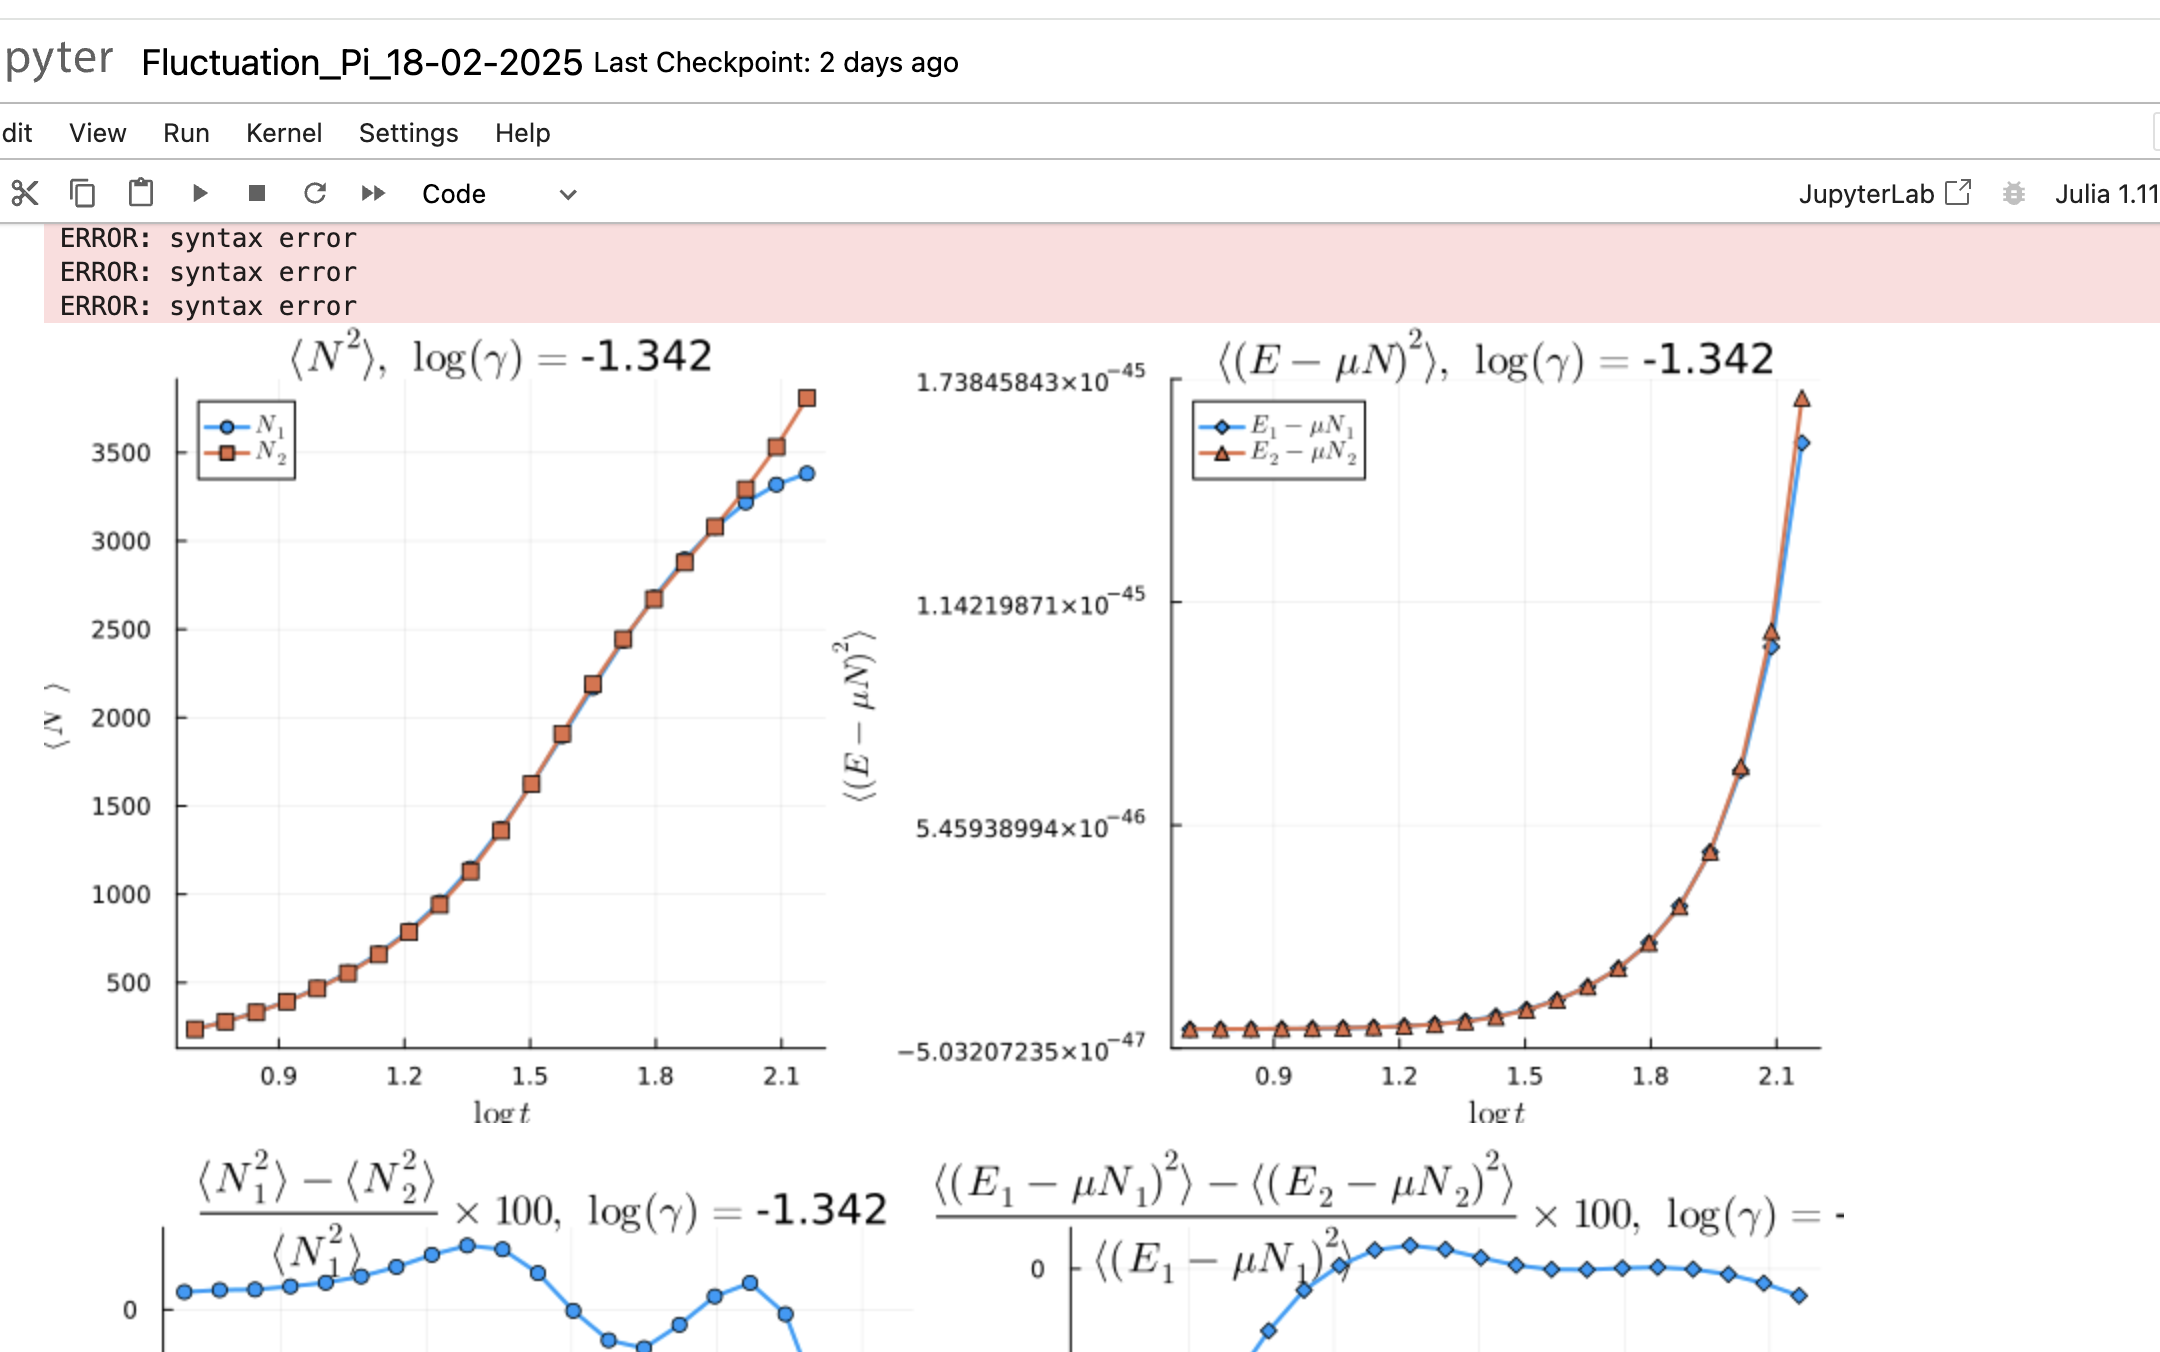
\includegraphics[width=1\textwidth]{Figures/test}

%\begin{aff}
%Donc une a l'ordre un en $\delta \theta (\operator{A}^{(0)})^{-1} %\operator{V}$ 

%\begin{eqnarray*}
%	\langle \delta \Pi ( \theta) \delta \Pi ( \theta') \rangle & = &  ( (\Pi^c_s - \Pi^c)\Pi^c/\Pi^c_s ) ( \theta ) \delta_{\theta, \theta'}/\delta \theta + \mathscr{F}(\theta , \theta' ) ,	
%\end{eqnarray*}

%avec 

%\begin{eqnarray*}
%	\mathscr{F}(\theta , \theta' ) & = & \left [ (\Pi^c_s - \Pi^c )( \theta)  +  (\Pi^c_s - \Pi^c ) ( \theta' )\right ] \frac{\Pi^c}{\Pi^c_s}(\theta)\frac{\Pi^c}{\Pi^c_s}(\theta') \frac{ \Delta( \theta'- \theta )}{ 2 \pi }\\
%	&&  - \left [ (\Pi^c_s - \Pi^c )( \theta)   (\Pi^c_s - \Pi^c ) ( \theta' )\right ] \frac{\Pi^c}{\Pi^c_s}(\theta)\frac{\Pi^c}{\Pi^c_s}(\theta')\int d\theta'' \left (   \frac{ \Pi^c/\Pi^c_s}{\Pi^c_s - \Pi^c} \right )(\theta'') \frac{\Delta(\theta''- \theta)}{2 \pi}\frac{\Delta(\theta''- \theta')}{2 \pi}  	
%\end{eqnarray*}
%\end{aff}



 











\subsection{Statistique des macro-états : entropie de Yang-Yang}

%\paragraph{Macro-états et entropie dans la TBA.}

%Dans la limite thermodynamique, dans le modèle statistique (GGE) , les moyenne, observables physiques deviennent des fonctionnelles de la {\bf distribution de rapidité}  $\rho(\theta)$ et du {\bf poing spectrale} $w(\theta)$ . Cette description est efficace car elle permet d’échapper au détail de chaque état propre. 
%Toutefois, cette simplification laisse en suspens une question cruciale : 
%Mais dans ce modelle qui simplifie on veux {\bf la distribution de rapidité d’un système à l'équilibre thermique à température finie} que l'on notera $\langle \rho \rangle$ pour dire la dansité moyenne. Et les lien entre  $w$ et $\langle \rho \rangle$.  Le problème est étudier par par Yang et Yang en 1969. Pour saisir l'enssentielle, nous devons comprendre la {\bf structure statistique des états propres} associés à une même distribution $\rho(\theta)$. Nous nous interrensons comme promis plus haut : à $\Omega(\theta)$ dans l'équation de moyenne \eqref{chap.2.moyenne.2}  ,  {\bf  nombre états propres microscopiques correspondent à une même distribution $\rho(\theta)$}.
%{\bf quelle est la distribution de rapidité d’un système à l'équilibre thermique à température finie ?}. 
%La question a été répondue dans les travaux pionniers de Yang et Yang (1969), que nous allons maintenant examiner brièvement. Pour répondre à cette question, nous devons comprendre la {\bf structure statistique des états propres} associés à une même distribution $\rho(\theta)$.

\paragraph{Motivation.}

Dans la limite thermodynamique, une observable locale dans un \textit{Generalized Gibbs Ensemble} (GGE) dépend uniquement de deux objets continus :  (i)  la \textbf{distribution de rapidité} $\rho(\theta)$, (ii) le \textbf{poids spectral} $w(\theta)$, c.-à-d.\ la " température généralisée " assignée à chaque quasi‑particule.
Cette reformulation est puissante car elle fait disparaître les détails d’un état propre individuel.  

\medskip
Cependant, pour décrire un \emph{vrai} équilibre à température finie, il faut la distribution à l'équilibre :
\begin{eqnarray*}
	\rho_{\mathrm{eq}}\;\doteq\;\langle \rho \rangle	 \quad \qquad\text{et son lien fonctionnel avec }w.
\end{eqnarray*}
%\[
%\boxed{\;
%  \rho_{\mathrm{eq}}\;=\;\langle \rho(\theta) \rangle
%\;}
%\qquad\text{et son lien fonctionnel avec }w(\theta).
%\]
La réponse fut donnée dans les travaux pionniers de \textsc{Yang \& Yang} (1969).  
Leur approche repose sur l’analyse de la \textbf{structure statistique des états propres} partageant la même distribution $\rho(\theta)$.

% : combien d’états microscopiquement distincts correspondent à ce même « macro‑état » ?

\paragraph{Distribution de rapidité comme macro-état.}

Chaque distribution de rapidité $\rho(\theta)$ ne correspond pas à un état propre unique, mais à un grand {\bf ensemble de micro-états} : différents choix des ensembles de quasi-moments $(\{\theta_a\}_{a \in \llbracket 1 , N \rrbracket })_{N \in \mathbb{Z}} $ peuvent conduire à la même densité de distribution à l’échelle macroscopique. Ainsi, $\rho(\theta)$ doit être interprétée comme un {\bf macro-état}, qui agrège un très grand nombre d’états propres microscopiques.

La question thermodynamique devient alors : {\bf Combien de micro-états microscopiquement distincts sont compatibles avec un même macro-état $\rho(\theta)$ ?} 

\medskip
Plus précisément, dans l’expression de moyenne des operateurs locaux \eqref{chap.2.moyenne.2}, apparaît le facteur
\(
\Omega[\rho]
\),
qui compte ces états propres.  
La détermination de $\Omega[\rho]$ (ou équivalemment de l’entropie de Yang–Yang $\mathcal{S}_{YY}[\rho]$ car 
\(
\Omega[\rho] = e^{L\mathcal{S}_{YY}[\rho]}
\)
avec $L$ la taille du système
) est donc la clé pour relier \emph{(i)} le poids spectral $w(\theta)$ imposé dans le GGE et \emph{(ii)} la distribution de rapidité moyenne $\rho_{\mathrm{eq}}(\theta)$ observée à l’équilibre.

\paragraph{Dénombrement local des configurations microcanoniques.}
Pour répondre à cette question, on subdivise l’axe des rapidités en petites tranches ou cellules de largeur $\delta \theta$, chacune centrée en un point $\theta_a$. Dans une tranche $[\theta_a, \theta_a + \delta\theta]$, on suppose que la densité $\rho(\theta)$ est à peu près constante. Le nombre de quasi-particules dans cette tranche est alors approximativement :
\begin{eqnarray*}
	N_a = L\rho(\theta_a) \delta \theta,
\end{eqnarray*}
et le nombre total d'états disponibles (i.e., le nombre d’états possibles si toutes les positions en moment étaient disponibles) est donné par la densité totale de niveaux 
\begin{eqnarray*}
	M_a = L\rho_s(\theta_a) \delta \theta.
\end{eqnarray*}
La densité de niveaux $\rho_s(\theta)$ tient compte du fait que les moments sont quantifiés de manière discrète, en raison des équations de Bethe (voir équation (??)).

Les particules occupent ces niveaux de manière analogue à des fermions libres (principe d’exclusion de Pauli), le nombre de manières différentes de choisir $N_a$ niveaux parmi $M_a$ est donné par :
	
	
	\begin{figure}[H]
		\centering 
		\begin{tikzpicture}
			%\def\Occupation{
	\def\traitx{0.3}
	\def\traity{0.5}
	\draw
		(-10.5 , 0 ) edge [thick,line width=0.8ex ]( -3.2  , 0 )
		( -3.2 - \traitx  , 0 - \traity ) edge [thick,line width=0.8ex ]( -3.2 + \traitx  , 0 + \traity  )
		( -2.8 - \traitx  , 0 - \traity ) edge [thick,line width=0.8ex ]( -2.8 + \traitx  , 0 + \traity  )
		(-2.8 , 0 ) edge [thick,line width=0.8ex ](2.8  , 0 )
		( 2.8 - \traitx  , 0 - \traity ) edge [thick,line width=0.8ex ]( 2.8 + \traitx  , 0 + \traity  )
		( 3.2 - \traitx  , 0 - \traity ) edge [thick,line width=0.8ex ]( 3.2 + \traitx  , 0 + \traity  )
		(3.2, 0 ) edge [thick,line width=0.8ex,->,>=triangle 45 , color = black ]node [pos=1.01,below  ]{\huge$a$}	( 11  , 0 )
	;
	
	
	% Graduation abcsisse 
	\foreach \r in { 0 ,... , 2   } {
		\ifnum\r=0
			\draw [color = gray  ]
				( \r  , -0.3 ) edge [thick,line width=0.5ex] node [pos=-0.5 ]{\large \r }	( \r  , 0.3 )
			;
			\filldraw [line width=0.5ex , color = red ,outer color=red,inner color=red ] 
				( \r  , 0 )  circle (4pt)
			;
		\else\ifnum\r>0
			\draw [color = gray  ]
				( \r  , -0.3 ) edge [thick,line width=0.5ex] node [pos=-0.5 ,right]{\large \r }	( \r  , 0.3 )
				( -\r  , -0.3 ) edge [thick,line width=0.5ex]node [pos=-0.5, left ]{\large -\r }	( -\r  , 0.3 ) 
			;
			\filldraw [ line width=0.5ex , color = red ,outer color=red,inner color=red ]
				( -\r  , 0 )  circle (5pt)
			;
			\filldraw [ line width=0.5ex , color = red ,outer color=red,inner color=red ] 
				( \r  , 0 )  circle (5pt)
			;
		\fi\fi
	}

	
	\def\nmax{6};
	\def\nsmax{10}; % les trous
	%\foreach \r in {\nmax + 1 ,...,\nsmax} { % proble dans le -\r 
	\foreach \r in {4 ,...,\nsmax} {
		\draw [color=gray] 
			(\r,-0.3) edge [thick,line width=0.5ex]  (\r,0.3)
			(-\r,-0.3) edge [thick,line width=0.5ex]  (-\r,0.3)
		;
		\filldraw [line width=0.5ex , color = red ,outer color=white,inner color=white ] (\r,0) circle (4pt);
		\filldraw [line width=0.5ex , color = red ,outer color=white,inner color=white] (-\r,0) circle (4pt);
	}
	
	
	\foreach \r in {4,...,\nmax} {
		\ifnum\r=\nmax
			\draw [color=gray] 
				(\r,-0.3) edge [thick,line width=0.5ex] node [pos=-0.5]{ $\frac{N}{2}$ } (\r,0.3)
				(-\r,-0.3) edge [thick,line width=0.5ex] node [pos=-0.5]{ $-\frac{N}{2}$ } (-\r,0.3)
			;
			\filldraw [line width=0.5ex , color = red ,outer color=red,inner color=red ] (\r,0) circle (4pt);
			\filldraw [line width=0.5ex , color = red ,outer color=red,inner color=red ] (-\r,0) circle (4pt);
		\else\ifnum\r>4
			%\def\nreste{\nmax-\r}
			\pgfmathtruncatemacro{\nreste}{\nmax-\r}

			\draw [color=gray] 
				(\r,-0.3) edge [thick,line width=0.5ex] node [pos=-0.5]{ $\frac{N}{2} - \nreste$ } (\r,0.3)
				(-\r,-0.3) edge [thick,line width=0.5ex] node [pos=-0.5]{$-\frac{N}{2}+\nreste$ } (-\r,0.3)
			;
			\filldraw [line width=0.5ex , color = red ,outer color=red,inner color=red ] (\r,0) circle (4pt);
			\filldraw [line width=0.5ex , color = red ,outer color=red,inner color=red ] (-\r,0) circle (4pt);
		\else
			\draw [color=gray] 
				(\r,-0.3) edge [thick,line width=0.5ex] (\r,0.3)
				(-\r,-0.3) edge [thick,line width=0.5ex] (-\r,0.3)
			;
			\filldraw [line width=0.5ex , color = red ,outer color=red,inner color=red ] (\r,0) circle (4pt);
			\filldraw [line width=0.5ex , color = red ,outer color=red,inner color=red ] (-\r,0) circle (4pt);
		\fi\fi
	}
	
	
			
}


\begin{scope}
	%\draw[help lines , width=1.5ex] (-8,-3) grid (8,3);\draw[help lines ,width=0.5ex , opacity = 0.5] (-3,-3) grid[step=0.1] (3,3));
	
	%\draw[help lines] 
	%	(-3,-3) edge[width=1.5ex] grid (3,3)	
	%	(-3,-3) edge[width=0.5ex , opacity = 0.5] grid (3,3)	
	%;
	\begin{scope}[shift={(0,1)},rotate=0,opacity=1,color=black]
		\Occupation	
		
		\node[anchor=east, font=\bfseries] at (-11, 0) {\color{red}\large (T = 0 )} ;	
	\end{scope}
	
	
	\begin{scope}[shift={(0,-1.0)},rotate=0,opacity=1,color=black]
		\Occupation
		
		\node[anchor=east, font=\bfseries] at (-11, 0) {\color{red}\large (T > 0 )} ;
		%\def\nmax{8};
	
		\def\r{1};
		\draw [color=gray] 
			(\nmax-\r-1,-0.3) edge [thick,line width=0.5ex]  (\nmax-\r-1,0.3)
			(-\nmax+\r,-0.3) edge [thick,line width=0.5ex]  (-\nmax+\r,0.3)
			;
		\filldraw [line width=0.5ex , color = red ,outer color=white,inner color=white ] (\nmax-\r-1,0) circle (4pt);
		\filldraw [line width=0.5ex , color = red ,outer color=white,inner color=white] (-\nmax+\r,0) circle (4pt);
	
		\def\r{-1};
		\draw [color=gray] 
			(\nmax-\r,-0.3) edge [thick,line width=0.5ex]  (\nmax-\r,0.3)
			(-\nmax+\r,-0.3) edge [thick,line width=0.5ex]  (-\nmax+\r,0.3)
			;
		\filldraw [line width=0.5ex , color = red ,outer color=red,inner color=red ] (\nmax-\r,0) circle (4pt);
		\filldraw [line width=0.5ex , color = red ,outer color=red,inner color=red] (-\nmax+\r,0) circle (4pt);
	
		\draw[line width=0.8ex , color = red ,->,>=latex] ( \nmax - 1.8  ,0.7) to[out=55,in=125] (\nmax + 0.8 ,0.7) ;
		\draw[line width=0.8ex , color = red ,->,>=latex] (-\nmax + 0.8 ,0.7) to[out=125,in=55] (-\nmax - 0.8 ,0.7);
	
	
	\end{scope}
	
	\begin{scope}[shift={(-10.5,3)},rotate=0,opacity=1,color=black]
	
	\begin{scope}[shift={(-0,0)},rotate=0,opacity=1,color=black]
	
		\draw[shift={(0,0)} ,line width=1ex,rounded corners = 1ex,color=\colorslide , opacity =1 ,fill=\colorslide!00 , pattern={north east lines} , pattern color=\colorslide!00 ]
			(0 , -1 ) rectangle (5,1)
		;
		
		\filldraw [line width=0.5ex , color = red ,outer color=red,inner color=red ] (0.5 , 0.5) circle (4pt); 
		\node[anchor=west, font=\bfseries] at (0.7, 0.5) {\color{\colorslide}\large : quasi-particule};
		
		\filldraw [line width=-0.5ex , color = red ,outer color=white,inner color=white ] (0.5 , -0.5) circle (4pt); 
		\node[anchor=west, font=\bfseries] at (0.7, -0.5) {\color{\colorslide}\large : hole} ;
	\end{scope}
	
	\begin{scope}[shift={(6,0)},rotate=0,opacity=1,color=black]	
		
		\draw[shift={(0,0)} ,line width=1ex,rounded corners = 1ex,color=\colorslide , opacity =1 ,fill=\colorslide!00 , pattern={north east lines} , pattern color=\colorslide!00 ]
			(0 , -1 ) rectangle (7.5,1)
		;
		
		\node[anchor=west] at (0.5, 0.5) {\color{\colorslide}\large $\rho$ };\node[anchor=west, font=\bfseries] at (0.9, 0.5) {\color{\colorslide}\large : quasi-particule distribution};
		
		\node[anchor=west] at (0.5, -0.5) {\color{\colorslide}\large $\rho_h$ };\node[anchor=west, font=\bfseries] at (0.9, -0.5) {\color{\colorslide}\large  : hole distribution};
		
	\end{scope}
	
	\begin{scope}[shift={(14.5,0)},rotate=0,opacity=1,color=black]	
		
		\draw[shift={(0,0)} ,line width=1ex,rounded corners = 1ex,color=\colorslide , opacity =1 ,fill=\colorslide!00 , pattern={north east lines} , pattern color=\colorslide!00 ]
			(0 , -0.5 ) rectangle (7.0,0.5)
		;
		
		\node[anchor=west] at (0.5, 0) {\color{\colorslide}\large $\rho_s = \rho + \rho_h $ };\node[anchor=west, font=\bfseries] at (2.5, 0) {\color{\colorslide}\large : density of states};
		
	\end{scope}
	
	
	\end{scope}


		
	
\end{scope}

	
			\begin{scope}[transform canvas={scale=0.6}]
			%% Définition des couleurs avec les codes HTML
\definecolor{colorOne}{HTML}{443E46}
\definecolor{colorTwo}{HTML}{F6DEB8}
\definecolor{colorThree}{HTML}{908CA4}
\definecolor{colorFour}{HTML}{57659E}
\definecolor{colorFive}{HTML}{C57284}
\definecolor{colorSix}{HTML}{FF5B69}

% Raccourcis pour les couleurs
\def\colorOne{colorOne}
\def\colorTwo{colorTwo}
\def\colorThree{colorThree}
\def\colorFour{colorFour}
\def\colorFive{colorFive}
\def\colorSix{colorSix}

\def\colorslide{blue!50!black}

\def\Occupation{
	\def\traitx{0.3}
	\def\traity{0.5}
	\draw[shift={(0,0)}]
		(-13.5 , 0 ) edge [thick,line width=0.8ex ]( -3.2  , 0 )
		( -3.2 - \traitx  , 0 - \traity ) edge [thick,line width=0.8ex ]( -3.2 + \traitx  , 0 + \traity  )
		( -2.8 - \traitx  , 0 - \traity ) edge [thick,line width=0.8ex ]( -2.8 + \traitx  , 0 + \traity  )
		(-2.8 , 0 ) edge [thick,line width=0.8ex ](2.8  , 0 )
		( 2.8 - \traitx  , 0 - \traity ) edge [thick,line width=0.8ex ]( 2.8 + \traitx  , 0 + \traity  )
		( 3.2 - \traitx  , 0 - \traity ) edge [thick,line width=0.8ex ]( 3.2 + \traitx  , 0 + \traity  )
		(3.2, 0 ) edge [thick,line width=0.8ex,->,>=triangle 45 , color = black ]node [pos=1.01,below  ]{\huge$\theta$}	( 13  , 0 )
	;
	\draw[shift={(0,0)}, color=\colorOne]
		(-10.5 , -1.5 ) edge [thick,line width=0.8ex , ->,>=triangle 45  ]( -10.5  , 4.5 )
	;
		
	\foreach \r in {1 , ... , 3 } {
%		\draw[
%		decoration={
%		markings,
%    	mark connection node=my node,
%    	mark=at position 0 with{\node [blue,transform shape] (my node) {\large \r};}},
%		color=gray, thick, 
%		line width=0.5ex] decorate { 
%            (-11.0, \r) -- (-10.1, \r )}
%        ;
        \draw[
			color=\colorOne,
			] 
            (-11.0, \r) edge[color=\colorThree , thick,line width=0.5ex] node [pos=-0.5 ]{\large\color{\colorFour} $\frac{\r}{\delta \theta}$ } (-10.3, \r )
        	;
	
	}
	

	
	% Graduation abcsisse 
	% Définitions des listes
% Definitions of the lists
\def\listetuple{-9/\theta_{1}, -8/\theta_{2} , -5/\theta_{3} , -2/\theta_{a-1} , 0/\theta_{a} , 1/\theta_{a+1} , 2/\theta_{a+2} ,  5/\theta_{N-4} , 7/\theta_{N-3},8/\theta_{N-1},9/\theta_{N} }
\def\listetrais{-12 , -11, -10, -9 , -8 , -7 ,  -6 , -5, -4.5,-4, -2 , -1, 0 , 0.5, 1, 2, 4 , 5 ,  6 , 7 , 8 ,8.5, 9 ,  10 , 11, 12 }

% Loop over listetrais
\foreach \r in \listetrais {
    % Initialize found variable to zero
    % Initialize found variable to zero
    %\pgfmathsetmacro\found{0}
    \global\def\found{0}
    \xdef\nomtheta{}
    
    % Check if \r is in listetuple
    \foreach \x/\y in \listetuple { 
        \ifdim \r pt=\x pt % If \r matches any \x in listetuple
            \global\def\found{1} ;
            \xdef\nomtheta{\y} % Set \nomtheta to the corresponding \y
            %\pgfmathsetmacro\found{1} % Set found to 1            
            %\global\pgfmathsetmacro\found{1}
        \fi
    }
    
    %\node [circle, draw, red] (A) at (\r, 2) {\found , $\nomtheta$};
    
    % Draw the line and display \nomtheta if found
    \ifnum\found=1
        \draw[color=\colorOne, thick, line width=0.5ex] 
            (\r, -0.3) -- (\r, 0.3) node[red , pos=-0.5] {\large $\nomtheta$};
         \filldraw[line width=0.5ex, color=\colorSix, outer color=\colorSix, inner color=\colorSix] 
            (\r, 0) circle (4pt);
    \else 
        % Draw without \nomtheta and add a blue circle if not found
        \draw[color=\colorOne, thick, line width=0.5ex] 
            (\r, -0.3) -- (\r, 0.3);
        \filldraw[line width=0.5ex, color=\colorSix, outer color=\colorTwo, inner color=\colorTwo] 
            (\r, 0) circle (4pt); 
    \fi
}

\def\listetrais{-9.5/\theta_{i-1}/2/3, -6.5/\theta_{i}/1/4  ,   -1.5/\theta_{j}/2/4 , 1.5/\theta_{j+1}/-1/3 , 3.5/\theta_{\ell-1}/1/3 , 6.5/\theta_{\ell}/3/4 , 9.5/\theta(\theta_{\ell+1})/-1/3 };



\foreach \r/\nomx/\y/\ys in \listetrais {
	\draw[
		decoration={
		markings,
    	mark connection node=my node,
    	mark=at position .5 with{\node [blue,transform shape] (my node) {\large \color{\colorFour} $\nomx$};}},
		color=\colorThree , thick, 
		line width=0.5ex] decorate { 
            (\r, 0.12) -- (\r, -1.2)}
        ;
     
     \ifdim \y pt > -1 pt 
     	\draw[
			decoration={
			markings,
    		mark connection node=my node,
    		mark=at position .5 with{\node [blue,transform shape] (my node) {\large \color{\colorFour} $\Pi(\nomx) $};}},
			color=\colorThree, thick, 
			line width=0.5ex] decorate { 
            (\r, \y) -- (\r +3, \y)}
        ;
        \draw[
			decoration={
			markings,
    		mark connection node=my node,
    		mark=at position .5 with{\node [blue,transform shape] (my node) {\large \color{\colorFive} $\Pi_s(\nomx) $};}},
			color=\colorFive, thick, 
			line width=0.5ex] decorate { 
            (\r, \ys) -- (\r +3, \ys)}
        ;
     \fi 
     \ifdim \r pt= -1.5 pt
     	\draw[
     		decoration={
			markings,
    		mark connection node=my node,
    		mark=at position .5 with{\node [blue,transform shape] (my node) {\large \color{\colorFour}  $\delta \theta $};},
    		%mark=at position 0.1  with {\arrow[blue, line width=0.5ex]{<}},
    		%mark=at position 1  with {\arrow[blue, line width=0.5ex]{>}}
    		},
        	color=\colorThree,
        	thick,
        	line width=0.5ex,
        	%arrows={Computer Modern Rightarrow[line cap=round]-Computer Modern Rightarrow[line cap=round]}
   			](\r, -1.2) edge[arrows={Computer Modern Rightarrow[line cap=round]-}] (\r + 0.4, -1.2)decorate {
    		(\r, -1.2) -- (\r + 3, -1.2)}(\r + 2, -1.2) edge[arrows={-Computer Modern Rightarrow[line cap=round]}] (\r + 3, -1.2)
    		;
    \fi
			
	
}


			
}


\begin{scope}
	%\draw[help lines , width=1.5ex] (-8,-3) grid (8,3);\draw[help lines ,width=0.5ex , opacity = 0.5] (-3,-3) grid[step=0.1] (3,3));
	
	%\draw[help lines] 
	%	(-3,-3) edge[width=1.5ex] grid (3,3)	
	%	(-3,-3) edge[width=0.5ex , opacity = 0.5] grid (3,3)	
	%;
	\begin{scope}[shift={(0,1)},rotate=0,opacity=1,color=black]
		\Occupation	
		
		%\node[anchor=east, font=\bfseries] at (-11, 0) {\color{red}\large (T = 0 )} ;	
	\end{scope}
	
	
	
	
	\begin{scope}[shift={(-10.5,7)},rotate=0,opacity=1,color=black]
	
	\begin{scope}[shift={(-0,0)},rotate=0,opacity=1,color=black]
	
		\draw[shift={(0,0)} ,line width=1ex,rounded corners = 1ex,color=\colorOne , opacity =1 ,fill=\colorOne!00 , pattern={north east lines} , pattern color=\colorOne!00 ]
			(0 , -1 ) rectangle (5,1)
		;
		

		\begin{scope}[shift={(0.5,0.5)}]
			\draw[color=\colorOne, thick, line width=0.5ex] 
            (0, -0.3) -- (0, 0.3) ;
            \filldraw[line width=0.5ex, color=\colorSix, outer color=\colorSix, inner color=\colorSix] 
            (0, 0) circle (4pt);
            
            \node[anchor=west, font=\bfseries] at (0.2, 0) {\color{\colorSix}\large : quasi-particule};
		\end{scope}
		
		\begin{scope}[shift={(0.5,-0.5)}]
			\draw[color=\colorOne, thick, line width=0.5ex] 
            (0, -0.3) -- (0, 0.3) ;
            \filldraw[line width=0.5ex, color=\colorSix, outer color=\colorTwo, inner color=\colorTwo] 
            (0, 0) circle (4pt);
            
            \node[anchor=west, font=\bfseries] at (0.2, 0) {\color{\colorSix}\large : hole};
		\end{scope}

	\end{scope}
	
	\begin{scope}[shift={(6,0)},rotate=0,opacity=1,color=black]	
		
		\draw[shift={(0,0)} ,line width=1ex,rounded corners = 1ex,color=\colorOne , opacity =1 ,fill=\colorOne!00 , pattern={north east lines} , pattern color=\colorOne!00 ]
			(0 , -1 ) rectangle (7.5,1)
		;
		
		\node[anchor=west] at (0.5, 0.5) {\color{\colorFour}\large $\Pi$ };\node[anchor=west, font=\bfseries] at (1, 0.5) {\color{\colorFour}\large : quasi-particule distribution};
		
		\node[anchor=west] at (0.5, -0.5) {\color{\colorFour}\large $\Pi_h$ };\node[anchor=west, font=\bfseries] at (1, -0.5) {\color{\colorFour}\large  : hole distribution};
		
	\end{scope}
	
	\begin{scope}[shift={(14.5,0)},rotate=0,opacity=1,color=black]	
		
		\draw[shift={(0,0)} ,line width=1ex,rounded corners = 1ex,color=\colorOne , opacity =1 ,fill=\colorOne!00 , pattern={north east lines} , pattern color=\colorOne!00 ]
			(0 , -0.5 ) rectangle (7.0,0.5)
		;
		
		\node[anchor=west] at (0.2, 0) {\color{\colorFour}\large ${\color{\colorFive}\Pi_s} = \Pi + \Pi_h $ } node[anchor=west , font=\bfseries] at (3.1 , 0 )  {\color{\colorFour}\large {\color{\colorFive} : density of states}};
		
	\end{scope}
	
	
	\end{scope}


		
	
\end{scope}

	
			\end{scope}
			
			\draw[color = red , scale = 0.5 , draw = none ] (-13.5 , -1) rectangle (13 , 10) ; 
				
			
		\end{tikzpicture}	
		\captionsetup{skip=10pt} % Ajoute de l’espace après la légende
	\end{figure}
	
	
\begin{eqnarray}
	\Omega(\theta_a) & \approx  & \binom{M_a}{N_a} ~= ~   \frac{[ L\rho_s ( \theta ) \delta \theta ] ! }{ [ L\rho ( \theta ) \delta \theta ] ! [( L\rho_s ( \theta ) - L\rho ( \theta ) )  \delta \theta ] ! }. 	
\end{eqnarray}

\paragraph{Estimation asymptotique à l’aide de Stirling.}

En utilisant la formule de Stirling :
\begin{eqnarray}
	n! & \underset{n \to \infty}{\sim} &  n^n e^{-n} \sqrt{2\pi n}.,
\end{eqnarray}	
composé du fonction logarithmique, il vient cette équivalence : 
\begin{eqnarray}
	\ln n! & \underset{n \to \infty}{\rightarrow} & n \ln n \underbrace{- n + \ln \sqrt{2 \pi n }}_{o \left ( n \ln n \right ) } ,\\
	&  \underset{n \to \infty}{\sim} & n \ln n  
\end{eqnarray}
	
$\# \mbox{conf.}$ est jamais null donc on peut approximer, pour de grandes valeurs de $L$ et de $\delta\theta$  : 
\begin{eqnarray}
    \ln \Omega(\theta) & \underset{\underset{\rho (\theta )\leq  \rho_s (\theta )}{\rho \delta \theta  \to \infty}}{\sim}   & L [ \rho_s\ln \rho_s - \rho \ln \rho - (\rho_s - \rho ) \ln ( \rho_s - \rho) ] (\theta )\delta \theta .
\end{eqnarray}

Cette expression donne la contribution par unité de $\theta$ à l’{\bf entropie}  associée à la cellule autour de $\theta_a$.

\paragraph{Entropie de Yang-Yang : définition .}
%L'entropie totale du macro-état $\rho(\theta)$, notée $\mathcal{S}_{YY}[\rho]$, est obtenue en sommant sur toutes les tranches. Pour alléger la notation, nous écrivons cette somme comme :
%Le nombre total de micro-états est le produit de toutes ces configurations pour toutes les cellules de rapidité $[\theta, \theta + \delta \theta]$. %En prenant le logarithme et en remplaçant la somme par une intégrale sur $ \theta$, nous obtenons l'entropie de Yang-Yang :

%L'entropie totale du macro-état $\rho(\theta)$, notée $\mathcal{S}_{YY}[\rho]$, est obtenue en sommant sur toutes les tranches. Pour alléger la notation, nous écrivons cette somme comme :
%Le nombre total de micro-états compatibles avec une distribution macroscopique $\rho(\theta)$ est donné par le produit des nombres de configurations pour chaque cellule de rapidité $[\theta, \theta + \delta \theta]$.

%En prenant la sum le logarithme des $\Omega(\theta)$ , on obtient l'entropie totale de Yang-Yang. Pour alléger la notation, cette somme sur les tranches est notée :

Le nombre total de micro-états compatibles avec une distribution macroscopique donnée $\rho(\theta)$ est obtenu en prenant le produit des nombres de configurations pour chaque cellule de rapidité $[\theta_a, \theta_a + \delta \theta]$ : $ \Omega(\theta_a)$ .
En prenant le logarithme de ce produit, on accède à l'entropie totale. Pour alléger la notation, cette somme sur les cellules est notée
\(
	\sum_a^{\theta-\mbox{\tiny cellules}}	
\)
où chaque $a$ indexe une cellule de rapidité $[\theta_a, \theta_a + \delta\theta]$.
On écrit alors :
\begin{eqnarray}
    \ln \Omega[\rho] & = & \sum_a^{\theta-\mbox{\tiny cellules}} \ln \Omega(\theta_a), \\
    & \approx &   L\mathcal{S}_{YY} [ \rho ] , 	
\end{eqnarray}
où l’on définit l’\textbf{entropie de Yang–Yang} par la formule discrétisée :
\begin{eqnarray}
    \mathcal{S}_{YY}[\rho] & \doteq & \sum_a^{\theta-\mbox{\tiny cellules}} \, [ \rho_s\ln \rho_s - \rho \ln \rho - ( \rho_s - \rho ) \ln ( \rho_s - \rho ) ] (\theta_a) \delta \theta .
\end{eqnarray}

%\paragraph{Énergie généralisée.}	
%Les variations de $w(\theta)$ étant négligeables sur chaque tranche de largeur $\delta\theta$, on peut approximer l’énergie généralisée comme :%  $\sum_{a = 1}^N  f(\theta_a) = \sum_{a \vert tranche } f(\theta_a) \Pi( \theta_a)\delta \theta$.

%\begin{eqnarray}
%	 \mathcal{W} & = & \sum_{a = 1}^N  w(\theta_a)	 ~ \sim ~ L\mathcal{W}[\rho] ~=~ L \sum_a^{\theta-\mbox{\tiny tranches}}	 w(\theta_a) \rho(\theta_a) \delta \theta.
%\end{eqnarray}

\paragraph{Énergie généralisée par unité de longueur : définition.}

Dans le cadre du Generalized Gibbs Ensemble (GGE), l’\textbf{énergie généralisée} associée à une distribution de rapidité $\rho(\theta)$ et à un poids spectral $w(\theta)$ est définie comme la somme des poids assignés à chaque quasi-particule. 
Dans la limite thermodynamique, en supposant que $w(\theta)$ varie lentement sur chaque tranche $[\theta_a, \theta_a + \delta\theta]$ ,  cette somme soit l’\textbf{énergie généralisée par unité de longueur} $\mathcal{W}$ se se définit par :
\begin{eqnarray}
	L \mathcal{W}(\{\theta_a\}) \doteq  \sum_{a = 1}^N w(\theta_a) 
	 \underset{\mbox{\tiny therm .}}{\sim}  L \mathcal{W}[\rho]  \doteq  L \sum_a^{\theta\text{-cellules}} w(\theta_a) \rho(\theta_a)\, \delta\theta. 
\end{eqnarray}

%La fonctionnelle
%\(
%\mathcal{W}[\rho] = \int d\theta\, w(\theta)\, \rho(\theta)
%\)
%représente donc l’énergie généralisée par unité de longueur, dans l’état macroscopique défini par la distribution $\rho$.


\paragraph{Moyenne des Observables locales dans la limite thermodynamique.}

Dans un ensemble général (GGE), la valeur moyenne de l’observable \eqref{chap.2.moyenne.2} devient :	
	
\begin{eqnarray}\label{chap.2.moyenne.3}
	\underset{\mbox{\tiny therm.}}{\lim} \langle \operator{\mathcal{O}} \rangle_{GGE} &  \approx &  ~ \frac{  \displaystyle \sum_{\rho }  \langle \operator{\mathcal{O}}\rangle_{[\rho]}  e^{L(\mathcal{S}_{YY}[\rho] -  \mathcal{W}[\rho]) }}{ \displaystyle \sum_{\rho } e^{L(\mathcal{S}_{YY}[\rho] -  \mathcal{W}[\rho]) } },
\end{eqnarray}
où la somme $\sum\rho$ porte sur toutes les distributions possibles de rapidité $\rho$

%%%%%%%%%%%%%%%%%%%%%%%%%%%%%%%%%%%%%%%%%
\paragraph{Passage à la limite continue.}
%En faisant tandre $\delta \theta \to 0 $ , les somme devienen des integrales 
En faisant tendre $\delta\theta \to 0$, les sommes deviennent des intégrales 
%\(
%\sum_a^{\theta-\mbox{\tiny tranches}}\delta \theta   \underset{\delta \theta \to 0 }{\rightarrow}  \int d \theta ,	
%\)
et l'entropie de Yang-Yang ainsi que l’énergie généralisée par unité de longueur prennent la forme :
\begin{eqnarray}
	\mathcal{S}_{YY}[\rho] & = & \int d \theta  \, [ \rho_s\ln \rho_s - \rho \ln \rho - ( \rho_s - \rho ) \ln ( \rho_s - \rho ) ] (\theta) , \label{chap.2.entropi.int}\\
	\mathcal{W}[\rho] & = & \int   w(\theta) \rho(\theta) \, d \theta \label{chap.2.W.int}		
\end{eqnarray}

%%%%%%%%%%%%%%%%%%%%%%%%%%%%%%%%%%%%%%%%%%
\paragraph{Formule fonctionnelle pour les moyennes.}

%et la valeur moyenne des opservables $\langle \operator{\mathcal{O}} \rangle$ s'écrit commes une intégrale de chemin/formelle
Dans la limite thermodynamique $L \to \infty$, la somme sur les distributions de rapidité $\rho$ admissibles peut être approximée par une intégrale fonctionnelle sur l’espace des densités de rapidité continues, munie d’une mesure fonctionnelle $\mathcal{D}\rho$ : 
\(
\sum_{\rho } \sim \int \mathcal{D} \rho .
\)
Cette correspondance repose sur l’idée que les macro-états admissibles deviennent denses dans l’espace fonctionnel, et que le poids statistique associé à chaque configuration est donné par l’entropie de Yang–Yang.
La mesure fonctionnelle $\mathcal{D}\rho$ parcourt l’espace des densités
$\rho(\theta)$ continues, \emph{chaque configuration étant pondérée par le
facteur exponentiel}
\(
e^{\,L(\mathcal{S}_{YY}[\rho]-\mathcal{W}[\rho])}.
\)
Finalement, la moyenne d'une observable dans le GGE \eqref{chap.2.moyenne.3} s’écrit comme une intégrale fonctionnelle/de chemin :
\begin{eqnarray}
	\underset{\mbox{\tiny therm.}}{\lim} \langle \operator{\mathcal{O}} \rangle_{GGE} & = & \frac{\int \mathcal{D} \rho \; e^{L (\mathcal{S}_{YY}[\rho] - \mathcal{W}[\rho])} \, \langle\operator{\mathcal{O}}\rangle_{[\rho]}}{\int \mathcal{D} \rho \; e^{L (\mathcal{S}_{YY}[\rho] - \mathcal{W}[\rho])}}. \label{chap:TBA:eq:ensemble_average}
\end{eqnarray}


%----------------------
%------------------------------------------------------------------
%\paragraph{Passage de la somme discrète à l’intégrale fonctionnelle.}

%Dans la limite thermodynamique $L\to\infty$, l’ensemble (discret) des
%distributions de rapidité admissibles devient dense dans l’espace
%fonctionnel ; la somme correspondante peut donc s’approximer par une
%intégrale fonctionnelle :
%\[
%\sum_{\rho}\; \longrightarrow\; \int\! \mathcal{D}\rho .
%\]
%La mesure fonctionnelle $\mathcal{D}\rho$ parcourt l’espace des densités
%$\rho(\theta)$ continues, \emph{chaque configuration étant pondérée par le
%facteur exponentiel}
%\(
%e^{\,L\bigl[\mathcal{S}_{YY}[\rho]-\mathcal{W}[\rho]\bigr]},
%\)
%qui combine
%\begin{itemize}
%\item l’\textbf{entropie de Yang–Yang}
%      $\displaystyle
%        \mathcal{S}_{YY}[\rho]
%        =\!\int d\theta\,
%          \bigl[
%            \rho_s\ln\rho_s
%            -\rho\ln\rho
%            -(\rho_s-\rho)\ln(\rho_s-\rho)
%          \bigr]$,
%\item le \textbf{coût énergétique généralisé}
%      $\displaystyle
%        \mathcal{W}[\rho]
%        =\!\int d\theta\, w(\theta)\,\rho(\theta)$,
%\end{itemize}
%où $w(\theta)$ est le \emph{poids spectral} fixé par le GGE.

%------------------------------------------------------------------
%\paragraph{Moyenne d’une observable dans le GGE.}

%On obtient alors la formule de champ moyen
%\begin{equation}\label{eq:GGE-functional-average}
%\bigl\langle\mathcal{O}\bigr\rangle_{\!{\rm GGE}}
%=
%\frac{\displaystyle
%      \int \mathcal{D}\rho\;
%      e^{L\bigl[\mathcal{S}_{YY}[\rho]-\mathcal{W}[\rho]\bigr]}\,
%      \langle\mathcal{O}\rangle_{[\rho]}}
%     {\displaystyle
%      \int \mathcal{D}\rho\;
%      e^{L\bigl[\mathcal{S}_{YY}[\rho]-\mathcal{W}[\rho]\bigr]}}.
%\end{equation}

%------------------------------------------------------------------
\paragraph{Interprétation thermodynamique.}

\begin{itemize}[label = $\bullet$] 
\item $\mathcal{S}_{YY}[\rho]$ \emph{compte} le logarithme du nombre de
      micro-états réalisant la distribution $\rho(\theta)$ :
      c’est l’\textbf{entropie combinatoire}.
\item $\mathcal{W}[\rho]$ mesure le \emph{coût énergétique généralisé}
      associé à cette distribution, dicté par le poids spectral $w(\theta)$.
\end{itemize}

Leur différence
\[
(\mathcal{S}_{YY}-\mathcal{W})[\rho]
\]
joue donc le rôle d’une \emph{fonction thermodynamique effective}
(analogue à une entropie libre).  
L’exposant $e^{L(\mathcal{S}_{YY}-\mathcal{W})[\rho]}$ fixe la \textbf{probabilité relative} d’un
macro-état $\rho(\theta)$ dans le GGE : le terme entropique favorise la
multiplicité des états, tandis que le terme énergétique pénalise les
configurations coûteuses — d’où la compétition caractéristique de
l’équilibre statistique.





%avec $\mathcal{O}[\rho]$ la valeur de l’observable dans un état propre caractérisé par la distribution de rapidité $\rho$.	
%où $\mathcal{O}[\rho]$ est la valeur de l’observable dans un état propre caractérisé par la distribution $\rho$.

%%Dans ce chapitre, nous nous intéressons aux fluctuations de la distribution de rapidité \( \delta \rho \) autour d'une distribution de référence \( \rho^c \), qui maximise la contribution à la fonction de partition des états, exprimée comme une fonctionnelle de la distribution \( \rho \) : 

La fonction de partition des états, s'exprime comme une fonctionnelle de la distribution \( \rho \) : 

\begin{eqnarray*}
	\Xi & = & \sum_\rho \exp \left( -\mathcal{A}(\rho) \right).
\end{eqnarray*}  

Dans la section {\em \bf Entropie de Yang-Yang} (\ref{??}), l'action \( \mathcal{A}(\rho) \) s'écrit sous la forme :  

\begin{eqnarray*}
	\mathcal{A}(\rho) & \doteq & - L\mathcal{S}_{YY}(\rho) + L\int f(\theta) \rho (\theta) \, d\theta,		
\end{eqnarray*}  

où \( \mathcal{S}_{YY} \) est la fonctionnelle d'entropie de Yang-Yang, définie dans (\ref{??}), et \( f \) est la fonction paramétrant les charges, introduite dans (\ref{??}).  

Dans cette même section {\em \bf Entropie de Yang-Yang} (\ref{??}), nous avons établi un lien entre \( f \) et distribution de référence \( \rho^c \), qui maximise la contribution à la fonction de partition des états .\\

On veux tester si nos experience est décrit pas un GGE. Pour cela nous nous intéressons aux fluctuations de la distribution de rapidité \( \delta \rho \) autour \( \rho^c \).

%Nous poursuivons à présent avec cette définition de l'action de classe $\mathcal{C}^2$ et admetant une distribution critique $\rho^c$ tel que sa différentielle en ce point critique soit nulle $d\mathcal{A}_{\rho^c} = 0 $ (\ref{??}) de sorte que d'aprés la formule de Taylor-Youg %afin de déterminer les fluctuations autour de \( \Pi^c \). Pour cela, nous réécrivons l'action sous la forme :  

Nous poursuivons à présent avec cette définition de l'action de classe $\mathcal{C}^2$ et admetant une distribution critique $\rho^c$ tel que sa différentielle en ce point critique soit nulle $d\mathcal{A}_{\rho^c} = 0 $ (\ref{??}) de sorte que d'aprés la formule de Taylor-Youg %afin de déterminer les fluctuations autour de \( \Pi^c \). Pour cela, nous réécrivons l'action sous la forme :  

\begin{eqnarray*}  
	\mathcal{A}(\rho^c + \delta \rho) & \underset{ \delta \rho \to 0 }{=} & \mathcal{A}(\rho^c)  + \frac{1}{2} \left. \frac{\delta^2 \mathcal{A}}{\delta \rho^2} \right|_{\rho^c} (\delta \rho) + \mathcal{O}((\delta \rho)^3),  
\end{eqnarray*}  

une expression quadratique pour l'action à l'ordre dominant en \( \delta \Pi \) avec $\left. \frac{\delta^2 \mathcal{A}}{\delta \rho^2} \right|_{\rho^c}$ la forme quadratique définie positive (Fig (\ref{fig.fluctu.A})).

\begin{figure}[H]
	\centering 
	\begin{tikzpicture}
		\begin{scope}[shift={(0,0)}]
			\begin{scope}[transform canvas={scale=0.6}]
				% Définition des couleurs avec les codes HTML
\definecolor{colorOne}{HTML}{443E46}
\definecolor{colorTwo}{HTML}{F6DEB8}
\definecolor{colorThree}{HTML}{908CA4}
\definecolor{colorFour}{HTML}{57659E}
\definecolor{colorFive}{HTML}{C57284}
\definecolor{colorSix}{HTML}{FF5B69}

% Raccourcis pour les couleurs
\def\colorOne{colorOne}
\def\colorTwo{colorTwo}
\def\colorThree{colorThree}
\def\colorFour{colorFour}
\def\colorFive{colorFive}
\def\colorSix{colorSix}

\def\colorslide{blue!50!black}



\begin{scope}
	% Tracer une courbe lisse entre des points
	\draw[shift={(0,0)} ,\colorOne]
		(-1 , 0 ) edge [thick,line width=0.8ex , ->,>=triangle 45  , \colorOne] node [pos = 1 , below ]{\huge$\rho$}( 5  , 0 )
	;
	\draw[shift={(0,0)}, color=\colorOne]
		(0, -1.0 ) edge [thick,line width=0.8ex , ->,>=triangle 45  ]node [pos=0.9,left=0.2cm ]{\huge$\mathcal{A}(\rho)$}( 0  , 5 )
	;
	\draw[]
		(2.5, 0.12 ) edge [thick,line width=0.8ex ,\colorThree ]node [pos=1,below  ]{\huge$\rho^c$} (2.5, -0.12 )	
	;
	
	\draw[]
		(2.5, -0.12 ) edge [thick,line width=0.4ex , dashed, \colorThree ] (2.5, 5.5 )
		(1.5, 1 ) edge [thick,line width=0.4ex , <->,>=triangle 45  , \colorThree ] (3.5, 1 )
		(-0.3,1) edge [thick,line width=0.4ex  , \colorThree ] node [pos=0,left ]{\huge$\mathcal{A}(\rho^c)$} (0.3, 1 )	
	;
    \draw[thick, line width=0.8ex , \colorFour] plot[smooth, tension=0.7] coordinates {
        (1, 5) (1.6 , 3 ) (2.5, 1) (3.5 , 3 )  (4, 5)
    };		
	
\end{scope}

	
			
			\end{scope}
			
			\draw[color = red , scale = 0.5 , draw = none  ] (-2 , -1) rectangle (5, 6) ; 	
		\end{scope}
		
		\begin{scope}[shift={(19,-1)}]
			\begin{scope}[transform canvas={scale=0.6}]
				% Définition des couleurs avec les codes HTML
\definecolor{colorOne}{HTML}{443E46}
\definecolor{colorTwo}{HTML}{F6DEB8}
\definecolor{colorThree}{HTML}{908CA4}
\definecolor{colorFour}{HTML}{57659E}
\definecolor{colorFive}{HTML}{C57284}
\definecolor{colorSix}{HTML}{FF5B69}

% Raccourcis pour les couleurs
\def\colorOne{colorOne}
\def\colorTwo{colorTwo}
\def\colorThree{colorThree}
\def\colorFour{colorFour}
\def\colorFive{colorFive}
\def\colorSix{colorSix}

\def\colorslide{blue!50!black}

\def\Occupation{
	\def\traitx{0.3}
	\def\traity{0.5}
	\draw[shift={(0,0)}]
		(-13.5 , 0 ) edge [thick,line width=0.8ex ]( -3.2  , 0 )
		( -3.2 - \traitx  , 0 - \traity ) edge [thick,line width=0.8ex ]( -3.2 + \traitx  , 0 + \traity  )
		( -2.8 - \traitx  , 0 - \traity ) edge [thick,line width=0.8ex ]( -2.8 + \traitx  , 0 + \traity  )
		(-2.8 , 0 ) edge [thick,line width=0.8ex ](2.8  , 0 )
		( 2.8 - \traitx  , 0 - \traity ) edge [thick,line width=0.8ex ]( 2.8 + \traitx  , 0 + \traity  )
		( 3.2 - \traitx  , 0 - \traity ) edge [thick,line width=0.8ex ]( 3.2 + \traitx  , 0 + \traity  )
		(3.2, 0 ) edge [thick,line width=0.8ex,->,>=triangle 45 , color = black ]node [pos=1.01,below  ]{\huge$\theta$}	( 13  , 0 )
	;
	\draw[shift={(0,0)}, color=\colorOne]
		(-10.5 , -1.5 ) edge [thick,line width=0.8ex , ->,>=triangle 45  ]( -10.5  , 4.5 )
	;
		
	\foreach \r in {1 , ... , 3 } {
%		\draw[
%		decoration={
%		markings,
%    	mark connection node=my node,
%    	mark=at position 0 with{\node [blue,transform shape] (my node) {\large \r};}},
%		color=gray, thick, 
%		line width=0.5ex] decorate { 
%            (-11.0, \r) -- (-10.1, \r )}
%        ;
        \draw[
			color=\colorOne,
			] 
            (-11.0, \r) edge[color=\colorThree , thick,line width=0.5ex] node [pos=-0.5 ]{\large\color{\colorFour} $\frac{\r}{\delta \theta}$ } (-10.3, \r )
        	;
	
	}
	

	
	% Graduation abcsisse 
	% Définitions des listes
% Definitions of the lists
\def\listetuple{-9/\theta_{1}, -8/\theta_{2} , -5/\theta_{3} , -2/\theta_{a-1} , 0/\theta_{a} , 1/\theta_{a+1} , 2/\theta_{a+2} ,  5/\theta_{N-4} , 7/\theta_{N-3},8/\theta_{N-1},9/\theta_{N} }
\def\listetrais{-12 , -11, -10, -9 , -8 , -7 ,  -6 , -5, -4.5,-4, -2 , -1, 0 , 0.5, 1, 2, 4 , 5 ,  6 , 7 , 8 ,8.5, 9 ,  10 , 11, 12 }

% Loop over listetrais
\foreach \r in \listetrais {
    % Initialize found variable to zero
    % Initialize found variable to zero
    %\pgfmathsetmacro\found{0}
    \global\def\found{0}
    \xdef\nomtheta{}
    
    % Check if \r is in listetuple
    \foreach \x/\y in \listetuple { 
        \ifdim \r pt=\x pt % If \r matches any \x in listetuple
            \global\def\found{1} ;
            \xdef\nomtheta{\y} % Set \nomtheta to the corresponding \y
            %\pgfmathsetmacro\found{1} % Set found to 1            
            %\global\pgfmathsetmacro\found{1}
        \fi
    }
    
    %\node [circle, draw, red] (A) at (\r, 2) {\found , $\nomtheta$};
    
    % Draw the line and display \nomtheta if found
    \ifnum\found=1
        \draw[color=\colorOne, thick, line width=0.5ex] 
            (\r, -0.3) -- (\r, 0.3) node[red , pos=-0.5] {\large $\nomtheta$};
         \filldraw[line width=0.5ex, color=\colorSix, outer color=\colorSix, inner color=\colorSix] 
            (\r, 0) circle (4pt);
    \else 
        % Draw without \nomtheta and add a blue circle if not found
        \draw[color=\colorOne, thick, line width=0.5ex] 
            (\r, -0.3) -- (\r, 0.3);
        \filldraw[line width=0.5ex, color=\colorSix, outer color=\colorTwo, inner color=\colorTwo] 
            (\r, 0) circle (4pt); 
    \fi
}

\def\listetrais{-9.5/\theta_{i-1}/2/3, -6.5/\theta_{i}/1/4  ,   -1.5/\theta_{j}/2/4 , 1.5/\theta_{j+1}/-1/3 , 3.5/\theta_{\ell-1}/1/3 , 6.5/\theta_{\ell}/3/4 , 9.5/\theta(\theta_{\ell+1})/-1/3 };



\foreach \r/\nomx/\y/\ys in \listetrais {
	\draw[
		decoration={
		markings,
    	mark connection node=my node,
    	mark=at position .5 with{\node [blue,transform shape] (my node) {\large \color{\colorFour} $\nomx$};}},
		color=\colorThree , thick, 
		line width=0.5ex] decorate { 
            (\r, 0.12) -- (\r, -1.2)}
        ;
     
     \ifdim \y pt > -1 pt 
     	\draw[
			decoration={
			markings,
    		mark connection node=my node,
    		mark=at position .5 with{\node [blue,transform shape] (my node) {\large \color{\colorFour} $\Pi(\nomx) $};}},
			color=\colorThree, thick, 
			line width=0.5ex] decorate { 
            (\r, \y) -- (\r +3, \y)}
        ;
        \draw[
			decoration={
			markings,
    		mark connection node=my node,
    		mark=at position .5 with{\node [blue,transform shape] (my node) {\large \color{\colorFive} $\Pi_s(\nomx) $};}},
			color=\colorFive, thick, 
			line width=0.5ex] decorate { 
            (\r, \ys) -- (\r +3, \ys)}
        ;
     \fi 
     \ifdim \r pt= -1.5 pt
     	\draw[
     		decoration={
			markings,
    		mark connection node=my node,
    		mark=at position .5 with{\node [blue,transform shape] (my node) {\large \color{\colorFour}  $\delta \theta $};},
    		%mark=at position 0.1  with {\arrow[blue, line width=0.5ex]{<}},
    		%mark=at position 1  with {\arrow[blue, line width=0.5ex]{>}}
    		},
        	color=\colorThree,
        	thick,
        	line width=0.5ex,
        	%arrows={Computer Modern Rightarrow[line cap=round]-Computer Modern Rightarrow[line cap=round]}
   			](\r, -1.2) edge[arrows={Computer Modern Rightarrow[line cap=round]-}] (\r + 0.4, -1.2)decorate {
    		(\r, -1.2) -- (\r + 3, -1.2)}(\r + 2, -1.2) edge[arrows={-Computer Modern Rightarrow[line cap=round]}] (\r + 3, -1.2)
    		;
    \fi
			
	
}


			
}


\begin{scope}
	%\draw[help lines , width=1.5ex] (-8,-3) grid (8,3);\draw[help lines ,width=0.5ex , opacity = 0.5] (-3,-3) grid[step=0.1] (3,3));
	
	%\draw[help lines] 
	%	(-3,-3) edge[width=1.5ex] grid (3,3)	
	%	(-3,-3) edge[width=0.5ex , opacity = 0.5] grid (3,3)	
	%;
	\begin{scope}[shift={(0,1)},rotate=0,opacity=1,color=black]
		\Occupation	
		
		%\node[anchor=east, font=\bfseries] at (-11, 0) {\color{red}\large (T = 0 )} ;	
	\end{scope}
	
	
	
	
	\begin{scope}[shift={(-10.5,7)},rotate=0,opacity=1,color=black]
	
	\begin{scope}[shift={(-0,0)},rotate=0,opacity=1,color=black]
	
		\draw[shift={(0,0)} ,line width=1ex,rounded corners = 1ex,color=\colorOne , opacity =1 ,fill=\colorOne!00 , pattern={north east lines} , pattern color=\colorOne!00 ]
			(0 , -1 ) rectangle (5,1)
		;
		

		\begin{scope}[shift={(0.5,0.5)}]
			\draw[color=\colorOne, thick, line width=0.5ex] 
            (0, -0.3) -- (0, 0.3) ;
            \filldraw[line width=0.5ex, color=\colorSix, outer color=\colorSix, inner color=\colorSix] 
            (0, 0) circle (4pt);
            
            \node[anchor=west, font=\bfseries] at (0.2, 0) {\color{\colorSix}\large : quasi-particule};
		\end{scope}
		
		\begin{scope}[shift={(0.5,-0.5)}]
			\draw[color=\colorOne, thick, line width=0.5ex] 
            (0, -0.3) -- (0, 0.3) ;
            \filldraw[line width=0.5ex, color=\colorSix, outer color=\colorTwo, inner color=\colorTwo] 
            (0, 0) circle (4pt);
            
            \node[anchor=west, font=\bfseries] at (0.2, 0) {\color{\colorSix}\large : hole};
		\end{scope}

	\end{scope}
	
	\begin{scope}[shift={(6,0)},rotate=0,opacity=1,color=black]	
		
		\draw[shift={(0,0)} ,line width=1ex,rounded corners = 1ex,color=\colorOne , opacity =1 ,fill=\colorOne!00 , pattern={north east lines} , pattern color=\colorOne!00 ]
			(0 , -1 ) rectangle (7.5,1)
		;
		
		\node[anchor=west] at (0.5, 0.5) {\color{\colorFour}\large $\Pi$ };\node[anchor=west, font=\bfseries] at (1, 0.5) {\color{\colorFour}\large : quasi-particule distribution};
		
		\node[anchor=west] at (0.5, -0.5) {\color{\colorFour}\large $\Pi_h$ };\node[anchor=west, font=\bfseries] at (1, -0.5) {\color{\colorFour}\large  : hole distribution};
		
	\end{scope}
	
	\begin{scope}[shift={(14.5,0)},rotate=0,opacity=1,color=black]	
		
		\draw[shift={(0,0)} ,line width=1ex,rounded corners = 1ex,color=\colorOne , opacity =1 ,fill=\colorOne!00 , pattern={north east lines} , pattern color=\colorOne!00 ]
			(0 , -0.5 ) rectangle (7.0,0.5)
		;
		
		\node[anchor=west] at (0.2, 0) {\color{\colorFour}\large ${\color{\colorFive}\Pi_s} = \Pi + \Pi_h $ } node[anchor=west , font=\bfseries] at (3.1 , 0 )  {\color{\colorFour}\large {\color{\colorFive} : density of states}};
		
	\end{scope}
	
	
	\end{scope}


		
	
\end{scope}

	
			
			\end{scope}
			\begin{scope}[scale=1]
				\draw[color = red , scale = 1 , draw = none  ] (-1 , -1) rectangle (5, 5) ; 
			\end{scope}	
		\end{scope}

		
				
			
	\end{tikzpicture}	
	\captionsetup{skip=10pt} % Ajoute de l’espace après la légende
	\label{fig.fluctu.A}
\end{figure}


On discrétise l'axe des rapidités en  petite cellule de rapidité $[\theta, \theta+\delta\theta]$, qui contient $L\rho(\theta) \delta \theta$ rapidités. 
	



Avec ces petites tranches, la forme quadratique s’écrit :

\begin{eqnarray*}
    \left. \frac{\delta^2 \mathcal{A}}{{\delta \rho}^2} \right|_{\rho^c}(\delta \rho ) &=&  \sum_{a,b \mid \text{tranche}}  
    \delta \rho(\theta_a)  \frac{\partial^2 \mathcal{A}}{\partial \delta \rho(\theta_a) \partial \delta \rho(\theta_b) } (\rho^c)  \delta \rho(\theta_b).
\end{eqnarray*}
Les fluctuations s’écrivent donc :

\begin{eqnarray*}
    \langle \delta \rho ( \theta) \delta \rho ( \theta') \rangle &=&  
    \frac{ \int d\delta \rho \, \delta \rho(\theta) \delta \rho ( \theta') 
    \exp \left( - \frac{1}{2} \sum_{a,b \mid \text{tranche}}  
    \delta \rho(\theta_a) \frac{\partial^2 \mathcal{A}}{\partial \delta \rho(\theta_a) \partial \delta \rho(\theta_b) } (\rho^c)  \delta \rho(\theta_b) \right) }
    { \int d\delta \Pi  
    \exp \left( - \frac{1}{2} \sum_{a,b \mid \text{tranche}}  
    \delta \rho(\theta_a) \frac{\partial^2 \mathcal{A}}{\partial \delta \rho(\theta_a) \partial \delta \rho(\theta_b) } (\rho^c)  \delta \rho(\theta_b) \right) } \\
    &=& \left( \mathbf{A}^{-1} \right)_{\theta , \theta'}
\end{eqnarray*}


\begin{aff}

\begin{eqnarray*}
	\langle \delta \rho ( \theta) \delta \rho ( \theta') \rangle &=& 	\left( \mathbf{A}^{-1} \right)_{\theta , \theta'}
\end{eqnarray*}

	
avec la  {\em matrice hessienne} $\mathbf{A}_{\theta , \theta'} \equiv \frac{\partial^2 \mathcal{A}}{\partial \delta \rho(\theta) \partial \delta \rho(\theta') }(\rho^c)$, au point critique/ qui maximise la probabilité  $\rho^c=\rho^c_s \nu^c $, s'écrit

\begin{eqnarray*}
	\operator{A} & = & \operator{A}^{(0)} + \delta \theta \operator{V}
\end{eqnarray*}

avec 

\begin{eqnarray*}
	A^{(0)}_{\theta , \theta'}  & = &  L\delta \theta \left ( \frac{ 1}{\rho^c_s ( 1  - \nu^c ) \nu^c } \right )(\theta)    \delta({\theta - \theta '})	,\\
	V_{\theta , \theta'}  &= & L \delta \theta \left \{ - \left [ \left ( \frac{1}{\rho^c_s( 1 - \nu^c) } \right ) ( \theta)  +  \left ( \frac{1}{\rho^c_s( 1 - \nu^c) } \right ) ( \theta' )\right ] \frac{ \Delta( \theta'- \theta )}{ 2 \pi } + \int d\theta''  \left ( \frac{\nu^c}{\rho^c_s( 1 - \nu^c) } \right )(\theta'') \frac{\Delta(\theta''- \theta)}{2 \pi}\frac{\Delta(\theta''- \theta')}{2 \pi}   \right \} 	
\end{eqnarray*}

\end{aff}

\subsection{Testes}

\begin{eqnarray*}
	\Delta_{\operator{\mathcal{N}}}^2  & = &  \frac{1}{\beta} \left . \frac{\partial \langle \operator{\mathcal{N}} \rangle}{\partial \mu} \right )_T \\
	\Delta_{\operator{\mathcal{E}}-\mu \operator{\mathcal{N}}}^2  & = &  - \left . \frac{\partial \langle \operator{\mathcal{E}}-\mu \operator{\mathcal{N}} \rangle}{\partial \beta} \right )_\mu 
\end{eqnarray*}

et 

\begin{eqnarray*}
	\Delta_{\operator{\mathcal{N}}}^2  &= & L^2 \int d\theta_a \int d \theta_b \, \langle \delta \rho(\theta_a) \delta \rho(\theta_b) \rangle \\
	\Delta_{\operator{\mathcal{E}}-\mu \operator{\mathcal{N}}}^2  & = & L^2 \int d\theta_a \int d \theta_b \, \left ( - \mu + \frac{1}2 m \theta_a^2  \right  )\left ( - \mu + \frac{1}2 m \theta_b^2  \right  )  \langle \delta \rho(\theta_a) \delta \rho(\theta_b) \rangle
\end{eqnarray*}

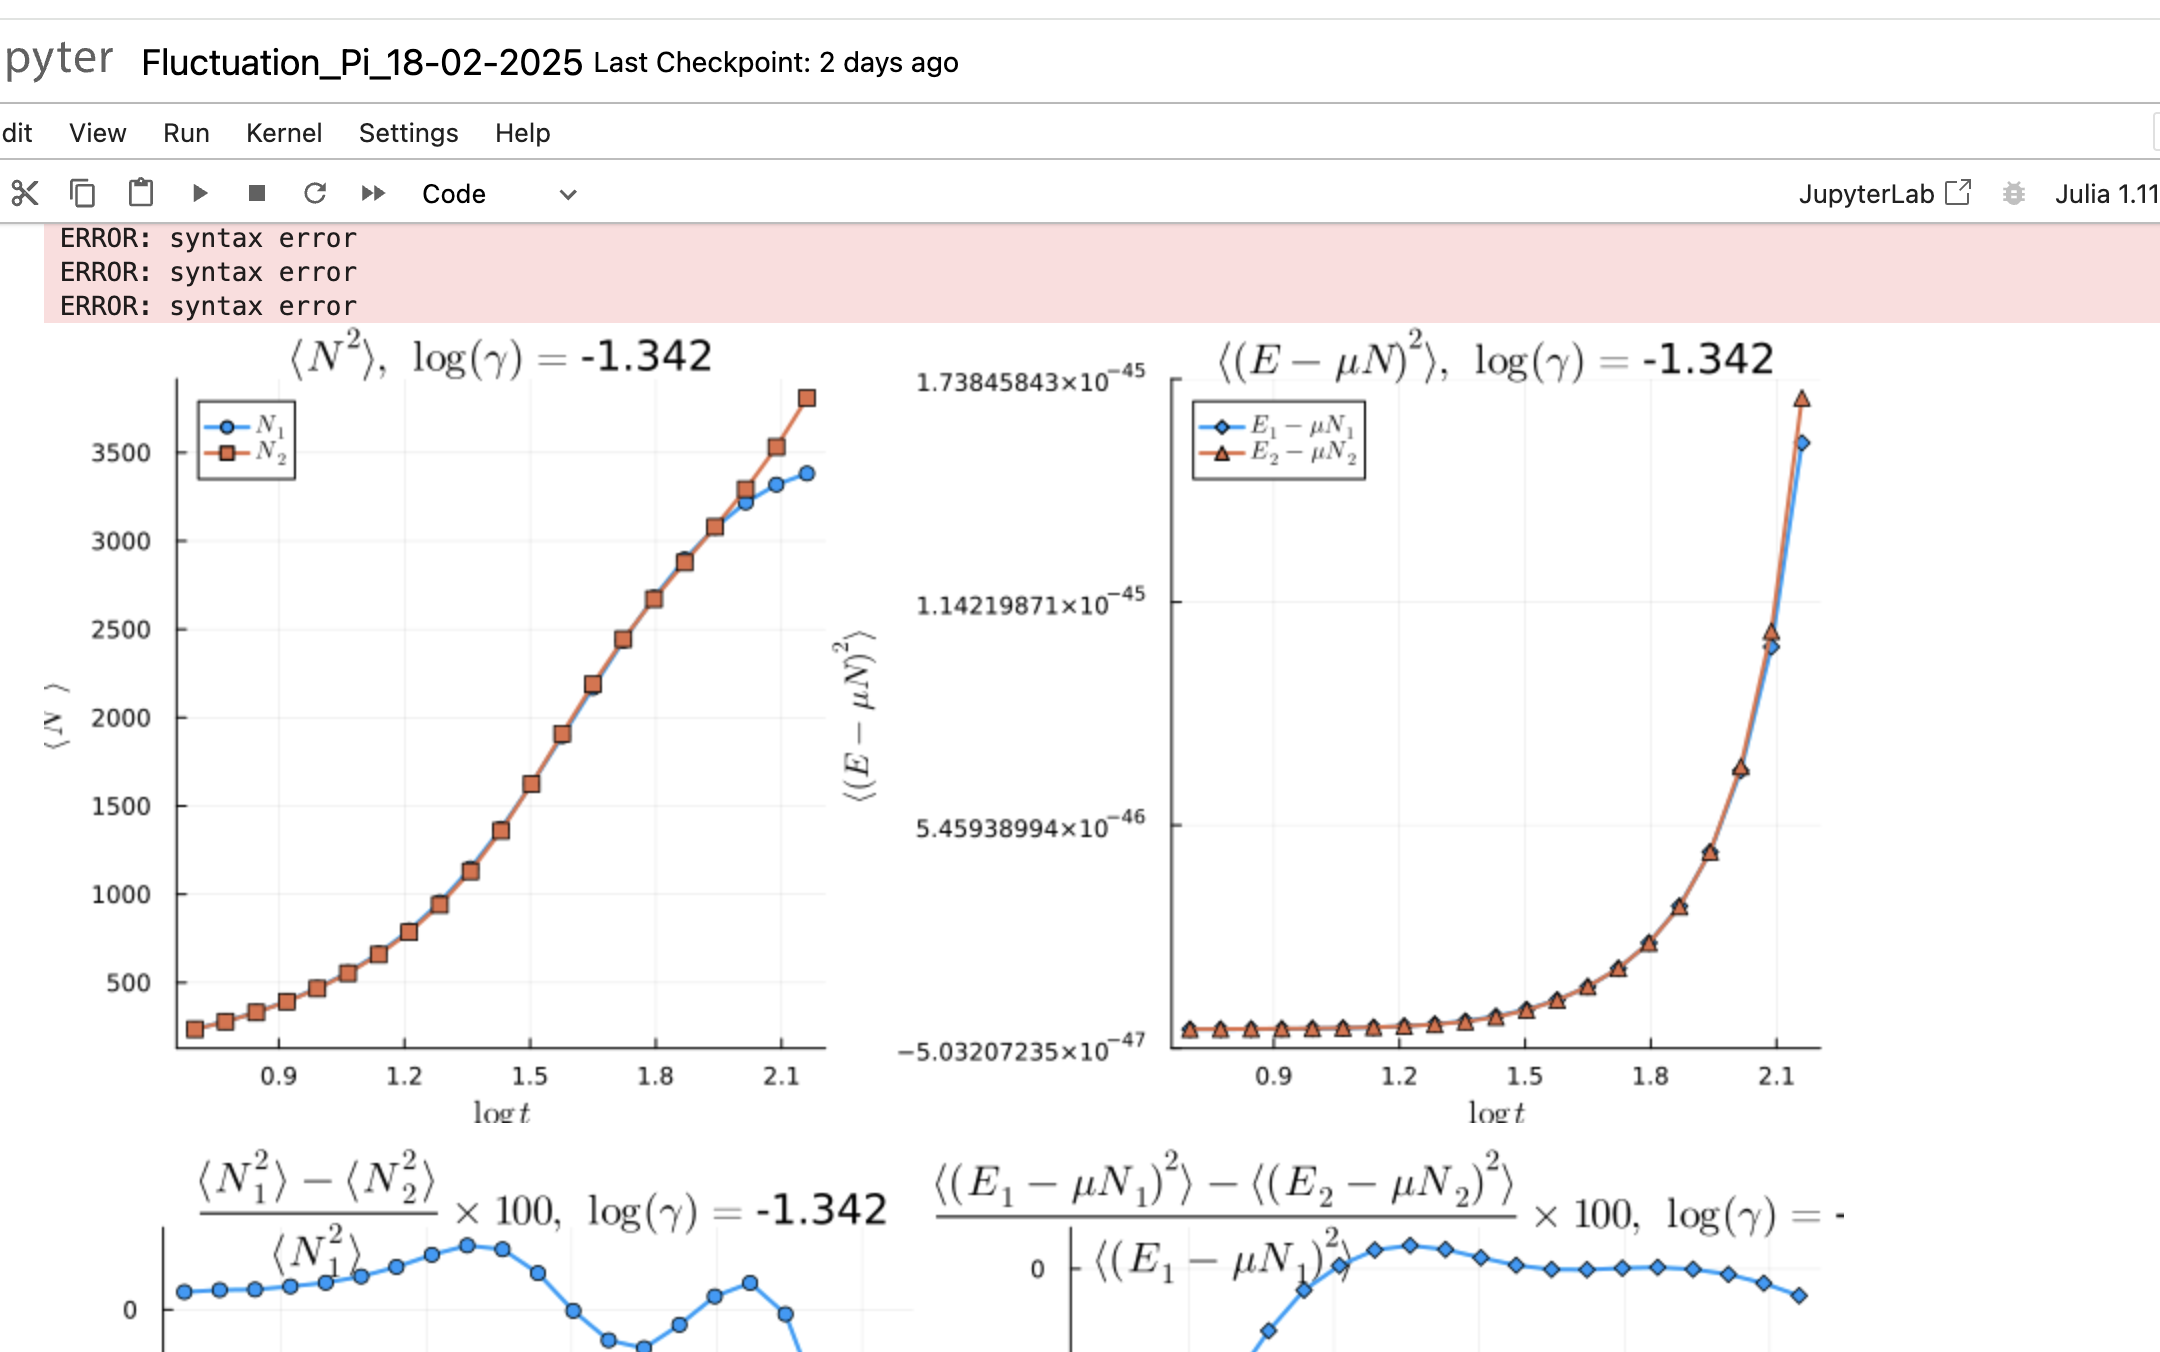
\includegraphics[width=1\textwidth]{Figures/test}

%\begin{aff}
%Donc une a l'ordre un en $\delta \theta (\operator{A}^{(0)})^{-1} %\operator{V}$ 

%\begin{eqnarray*}
%	\langle \delta \Pi ( \theta) \delta \Pi ( \theta') \rangle & = &  ( (\Pi^c_s - \Pi^c)\Pi^c/\Pi^c_s ) ( \theta ) \delta_{\theta, \theta'}/\delta \theta + \mathscr{F}(\theta , \theta' ) ,	
%\end{eqnarray*}

%avec 

%\begin{eqnarray*}
%	\mathscr{F}(\theta , \theta' ) & = & \left [ (\Pi^c_s - \Pi^c )( \theta)  +  (\Pi^c_s - \Pi^c ) ( \theta' )\right ] \frac{\Pi^c}{\Pi^c_s}(\theta)\frac{\Pi^c}{\Pi^c_s}(\theta') \frac{ \Delta( \theta'- \theta )}{ 2 \pi }\\
%	&&  - \left [ (\Pi^c_s - \Pi^c )( \theta)   (\Pi^c_s - \Pi^c ) ( \theta' )\right ] \frac{\Pi^c}{\Pi^c_s}(\theta)\frac{\Pi^c}{\Pi^c_s}(\theta')\int d\theta'' \left (   \frac{ \Pi^c/\Pi^c_s}{\Pi^c_s - \Pi^c} \right )(\theta'') \frac{\Delta(\theta''- \theta)}{2 \pi}\frac{\Delta(\theta''- \theta')}{2 \pi}  	
%\end{eqnarray*}
%\end{aff}



 








\subsection{Équations intégrales de la TBA}

\paragraph{Moyenne des observables dans l’ensemble généralisé de Gibbs.}

\paragraph{Approximation au point selle («\,méthode de la selle statique\,»)}

Dans la limite thermodynamique \( L \to \infty \), cette intégrale est dominée par la configuration \( \rho_{eq} \) qui maximise le poids exponentiel $e^{L(\mathcal{S}_{YY}-\mathcal{W})[\rho]}$  dans l'expression \eqref{chap:TBA:eq:ensemble_average}. Il s’agit de la densité de rapidité la plus probable, solution d’un problème de maximisation. On obtient à l’ordre principal
\begin{eqnarray}
	\underset{\mbox{\tiny therm.}}{\lim} \langle \operator{\mathcal{O}} \rangle_{GGE} & \approx &  \langle\operator{\mathcal{O}}\rangle_{[\rho_{eq} ]}.	
	\label{chap:TBA:eq:ensemble_average:approx}
\end{eqnarray}

Cette approximation correspond à une méthode de \textit{selle statique}, où l’on développe la \emph{fonction thermodynamique effective}, $\mathcal{S}_{YY}-\mathcal{W}$  au voisinage de la distribution dominante.


\paragraph{Développement fonctionnel au premier ordre.}

%On effectue un développement de Taylor fonctionnel de l'action à l’ordre linéaire en $\rho = \rho_{eq} + \delta \rho$ :
Écrivons
\(
\rho=\rho_{\text{eq}}+\delta\rho
\)
et développons $(\mathcal{S}_{YY}-\mathcal{W})[\rho]$ à l’ordre linéaire :
\begin{eqnarray*}
	\mathcal{S}_{YY}[\rho] - \mathcal{W}[\rho] & \approx & \mathcal{S}_{YY}[ \rho_{eq}] - \mathcal{W}[ \rho_{eq}] +  \left. \frac{\delta (\mathcal{S}_{YY}[\rho] - \mathcal{W}[\rho]) }{\delta \rho} \right|_{\rho = \rho_{eq} }	(\delta \rho) + \mathcal{O}(\delta \rho^2 ) ,
	\label{chap:TBA:eq:action}	
\end{eqnarray*}	
La condition de stationnarité au point selle impose :
\(
	\left. \frac{\delta (\mathcal{S}_{YY}[\rho] - \mathcal{W}[\rho]) }{\delta \rho} \right|_{\rho = \rho_{eq} }	  =  0  	
\)
soit 
\begin{equation}
\left. \frac{\delta \mathcal{S}_{YY}}{\delta \rho} \right|_{\rho = \rho_{eq}} = \left. \frac{\delta \mathcal{W}}{\delta \rho} \right|_{\rho = \rho_{eq}}. \label{chap:TBA:eq:stationnarite}
\end{equation}

%%%%%%%%%%%%%%%%
%-----------------------------------------------------

%------------------------------------------------------------------
%\subsection{Équations intégrales de la TBA}

%\paragraph{Moyenne des observables dans le Generalized Gibbs Ensemble.}

%Dans la limite thermodynamique, la moyenne d’une observable locale
%s’écrit formellement comme une intégrale fonctionnelle sur les densités de
%rapidité\,\footnote{%
%La mesure fonctionnelle $\mathcal{D}\rho$ est la limite continue de la
%somme discrète sur les macro-états admissibles, chacun étant pondéré par
%le facteur combinatoire $e^{L\mathcal{S}_{YY}[\rho]}$.}
%
%\begin{equation}\label{eq:TBA:ensemble_average}
%\left\langle \mathcal{O} \right\rangle_{\!\text{GGE}}
%=\frac{\displaystyle
%      \int\!\mathcal{D}\rho\;
%      e^{L\bigl[\mathcal{S}_{YY}[\rho]-\mathcal{W}[\rho]\bigr]}\;
%      \langle\mathcal{O}\rangle_{[\rho]}}
%     {\displaystyle
%      \int\!\mathcal{D}\rho\;
%      e^{L\bigl[\mathcal{S}_{YY}[\rho]-\mathcal{W}[\rho]\bigr]}} .
%\end{equation}

%------------------------------------------------------------------
%\paragraph{Approximation au point selle («\,méthode de la selle statique\,»).}

%Lorsque $L\to\infty$, les intégrales \eqref{eq:TBA:ensemble_average}
%sont dominées par la distribution
%$\rho_{\text{eq}}$ qui \emph{maximise} l’exposant
%\(
%\Phi[\rho]=\mathcal{S}_{YY}[\rho]-\mathcal{W}[\rho].
%\)
%On obtient à l’ordre principal
%\begin{equation}
%\left\langle \mathcal{O} \right\rangle_{\!\text{GGE}}
%\;\simeq\;
%\langle \mathcal{O} \rangle_{[\rho_{\text{eq}}]} .
%\label{eq:TBA:saddle_average}
%\end{equation}

%------------------------------------------------------------------
%\paragraph{Condition de stationnarité et équation variationnelle.}

%Écrivons
%\(
%\rho=\rho_{\text{eq}}+\delta\rho
%\)
%et développons $\Phi[\rho]$ à l’ordre linéaire :
%\[
%\Phi[\rho]\;=\;
%\Phi[\rho_{\text{eq}}]
%+
%\int d\theta\,
%\left.
%\frac{\delta\Phi}{\delta\rho(\theta)}
%\right|_{\rho_{\text{eq}}}
%\delta\rho(\theta)
%+O(\delta\rho^{2}).
%\]
%La stationnarité impose
%\(
%\dfrac{\delta\Phi}{\delta\rho(\theta)}\bigl|_{\rho_{\text{eq}}}=0,
%\)
%soit
%\begin{equation}
%\left.
%\frac{\delta\mathcal{S}_{YY}}{\delta\rho(\theta)}
%\right|_{\rho_{\text{eq}}}
%=
%\left.
%\frac{\delta\mathcal{W}}{\delta\rho(\theta)}
%\right|_{\rho_{\text{eq}}}.
%\label{eq:TBA:variational_condition}
%\end{equation}

%------------------------------------------------------------------
%\paragraph{Forme explicite : introduction de la pseudo-énergie.}

%Pour le modèle de Lieb–Liniger (et, plus généralement, pour un modèle
%intégrable à noyau $\Delta$), on introduit la \emph{pseudo-énergie}
%\[
%\varepsilon(\theta)
%\;=\;
%w(\theta)
%\;+\;\Bigl[\Delta\star\ln\!\bigl(1+e^{-\varepsilon}\bigr)\Bigr](\theta),
%\]
%obtenue en réécrivant \eqref{eq:TBA:variational_condition}.
%Le \emph{facteur d’occupation}
%\(
%\nu(\theta)=\rho(\theta)/\rho_s(\theta)
%\)
%se donne alors par la statistique de type Fermi-Dirac
%\[
%\nu(\theta)=\frac1{1+e^{\varepsilon(\theta)}}.
%\]

%Les équations intégrales complètes de la \textbf{Thermodynamique de Bethe}
%(TBA) sont donc
%\begin{align}
%2\pi\rho_s(\theta) &= 1 + \bigl[\Delta \star \rho\bigr](\theta),
%\label{eq:TBA:rho_s}\\[4pt]
%\rho(\theta) &= \frac{\rho_s(\theta)}{1+e^{\varepsilon(\theta)}},
%\qquad
%\varepsilon(\theta)=w(\theta)+\bigl[\Delta\star\ln(1+e^{-\varepsilon})\bigr](\theta).
%\label{eq:TBA:epsilon}
%\end{align}
%Elles déterminent sans ambiguïté la distribution d’équilibre
%$\rho_{\text{eq}}(\theta)$ en fonction du poids spectral $w(\theta)$.

%\medskip
%Ainsi, la méthode du point selle relie le \emph{poids spectral}
%(caractéristique du GGE) à la distribution de rapidité la plus probable,
%et permet d’évaluer les observables par la formule
%\label{chap:TBA:eq:ensemble_average:approx}.


%-----------------------------------------------------
%%%%%%%%%%%%%%%%

%\paragraph{Équation intégrale de la TBA.}

%Cette égalité donne naissance à une équation intégrale pour le poids spectral \( w \), défini comme la dérivée fonctionnelle de l'énergie généralisée pris en $\rho_{eq}$ :
%\(
%w ~=~ \left. \frac{\delta \mathcal{W}[\rho]}{\delta \rho} \right|_{\rho =  \rho_{eq} }
%\)
%qui par stationnarité (cf équation \eqref{chap:TBA:eq:stationnarite}) est égale à la dérivée fonctionnelle de l'entropie de Yang-Yang pris en $\rho_{eq}$ :
%\(
%\left. \frac{\delta \mathcal{S}_{YY}[\rho]}{\delta \rho} \right|_{\rho = \rho_{eq} }
%\) 
%qui lui vaux 
%\(
%\ln ( \nu_{eq}^{-1}  - 1 ) - \frac{\Delta}{2\pi} \star \ln ( 1 -  \nu_{eq })
%\)
%avec le facteur d'ocupation à l'équilibre $\nu_{eq} = \rho_{eq}/{\rho_{eq}}_s$. Ainci on peux s'arreter sur l'équation 
%\begin{eqnarray}
%	w & = & \ln ( \nu_{eq}^{-1}  - 1 ) - \frac{\Delta}{2\pi} \star \ln ( 1 -  \nu_{eq }).\label{chap:TBA:eq:w}
%\end{eqnarray}

%\medskip
%Ainsi, la méthode du point selle relie le \emph{poids spectral}
%(caractéristique du GGE) à la distribution de rapidité la plus probable,
%et permet d’évaluer les observables par la formule
%\eqref{chap:TBA:eq:ensemble_average:approx}.\\

%\paragraph{Forme explicite : introduction de la pseudo-énergie.}

%Le \emph{facteur d’occupation}
%\(
%\nu_{eq}
%\)
%se donne alors par la statistique de type Fermi-Dirac
%\begin{eqnarray}
%	\nu_{eq}=\frac1{1+e^{\epsilon}},\label{chap:TBA:eq:nu_eq}
%\end{eqnarray}
%où \emph{pseudo-énergie} 
%\(
%\epsilon
%\)
%se définie en intectant \eqref{chap:TBA:eq:nu_eq} dans \eqref{chap:TBA:eq:w} : 
%\begin{eqnarray}
%	\epsilon & = & w + \frac{\Delta}{2\pi} \star \ln ( 1  + e^{-\epsilon}).\label{chap:TBA:eq:e}	
%\end{eqnarray}


%---------------------------------
%------------------------------------------------------------------
\paragraph{Équation intégrale de la TBA.}

La condition de stationnarité au point selle \(\rho=\rho_{\mathrm{eq}}\) \eqref{chap:TBA:eq:stationnarite} implique :
\begin{eqnarray}
	\left.\frac{\delta\mathcal{S}_{YY}}{\delta\rho(\theta)}\right|_{\rho_{\mathrm{eq}}} = \left.\frac{\delta\mathcal{W}}{\delta\rho(\theta)}\right|_{\rho_{\mathrm{eq}}}\;\doteq\;w(\theta),
\end{eqnarray}
En utilisant l’expression explicite de l’entropie de Yang–Yang \eqref{chap.2.entropi.int}, on obtient l’identité fonctionnelle
\begin{eqnarray}
	w & = & \ln ( \nu_{\!eq}^{-1}  - 1 ) - \frac{\Delta}{2\pi} \star \ln ( 1 -  \nu_{\!eq}).\label{chap:TBA:eq:w}
\end{eqnarray}
où
\(
\nu_{\!eq}=\rho_{\!eq}/\rho_{s,\!eq}
\)
est le \textbf{facteur d’occupation} à l’équilibre.
%------------------------------------------------------------------
\paragraph{Forme pseudo-énergie.}
La \textbf{pseudo-énergie} $\epsilon$ se donne alors par la statistique de type Fermi-Dirac
\begin{eqnarray}
	\beta \epsilon =\ln(\nu^{-1}_{\!eq}-1),\qquad\nu_{\!eq}=\frac{1}{1+e^{\beta \epsilon}}.\label{chap:TBA:eq:nu}%\tag{\text{TBA--$\nu$}} 
\end{eqnarray}
En réinjectant \eqref{chap:TBA:eq:nu} dans \eqref{chap:TBA:eq:w} on obtient
l’équation intégrale canonique de la thermodynamique de Bethe :
\begin{eqnarray}
	\beta \epsilon & = & w - \frac{\Delta}{2\pi} \star \ln ( 1  + e^{-\beta \epsilon}).\label{chap:TBA:eq:e}%\tag{\text{TBA–-$\varepsilon$}}	
\end{eqnarray}
%\[
%\boxed{\;
%\varepsilon(\theta)
%=
%w(\theta)
%+\frac{\Delta}{2\pi}\star\ln\!\bigl[1+e^{-\varepsilon(\theta)}\bigr]
%\;}
%\tag{TBA–$\varepsilon$}\label{eq:TBA:eq:e}
%\]

Les relations \eqref{chap:TBA:eq:nu}–\eqref{chap:TBA:eq:e} déterminent de façon univoque la distribution de rapidité d’équilibre \(\rho_{\!eq}\) à partir du poids spectral \(w\), caractéristique du GGE.

\medskip
Ainsi, la méthode du point selle relie \emph{explicitement} le {\em poids spectral}, $w$  (caractéristique du GGE) au \emph{macro-état le plus probable}, $\rho_{eq}$ , et permet d’évaluer les observables par la formule d’ensemble \eqref{chap:TBA:eq:ensemble_average:approx}.


\paragraph{Résolution numérique de l’équation TBA.}

On se place à l’équilibre canonique, caractérisé par la température \( T \) et le potentiel chimique \( \mu \).  Dans ce cadre, le poids spectral vaut
\begin{equation}
  w(\theta)=\beta\bigl[\varepsilon(\theta)-\mu\bigr],\qquad\beta=\tfrac1T\; (k_B = 1 ),\quad\varepsilon(\theta)=\tfrac{\theta^{2}}{2}\;(m=1).\label{eq:TBA:w:canonical}
\end{equation}
En injectant \eqref{eq:TBA:w:canonical} dans l’équation intégrale pour lapseudo-énergie \eqref{chap:TBA:eq:e}, on obtient l’équation non linéaire :
\begin{eqnarray*}
	\beta \epsilon & = & \beta (\varepsilon - \mu)  -  \frac{\Delta}{2\pi} \star \ln \left( 1 + e^{-\beta \epsilon} \right) ,\label{eq:num:TBA}
\end{eqnarray*}
Cette équation définit un opérateur contractant sur l’espace des fonctions
\( \varepsilon(\theta) \) ; son Jacobien a une norme strictement
inférieure à 1, garantissant la convergence de l’itération de Picard.

\medskip
\subparagraph{Algorithme d’itération.}  
La structure contractante de l’équation garantit l’absence de cycles ou de points fixes multiples, assurant la convergence de l’itération vers l’unique solution admissible.
L’équation \eqref{eq:num:TBA} est non linéaire ; pour la résoudre numériquement, on utilise une méthode itérative de type Picard. On initialise
\(
  \epsilon_0 = \epsilon - \mu,
\)
puis on construit une suite de fonctions \(\varepsilon_n\) définie par
\begin{eqnarray*}
	\beta \epsilon_{n+1} & = & \beta \epsilon_0 -   \frac{\Delta}{2\pi} \star \ln \left( 1 + e^{-\beta \epsilon_n} \right) ,\quad n\ge0
\end{eqnarray*}
L’itération est poursuivie jusqu’à convergence, que l’on peut tester via le critère numérique
\(
  \beta \left\| \varepsilon_{n+1} - \varepsilon_n \right\|_\infty < 10^{-12},
\)
où \(\|\cdot\|_\infty\) désigne la norme \(L^\infty\) (ou un maximum discret après discrétisation).


\medskip
\subparagraph{Facteur d’occupation et densités.}  
Une fois la pseudo-énergie \( \epsilon(\theta) \) convergée, le facteur d’occupation  à l'équilibre est obtenu en injectant $\epsilon$ dans l’équation \eqref{chap:TBA:eq:nu}, ce qui donne  $\nu_{\!eq}$.
 
On en déduit ensuite la densité d'état à l'équilibre $\rho_{s,eq}$ via le {\bf dressing}  de la fonction constante $f(\theta) = 1$, selon \eqref{eq:TBA-rhos-2}, rappelée ici pour mémoire : $ 2\pi \rho_{s,eq}  =  1^{\mathrm{dr}}_{[\nu_{\! eq}]}$.\\

L’opérateur de dressing \eqref{eq:dressing} étant linéaire, il se résout numériquement sous la forme :
\begin{eqnarray*}
	\left\{ \mathrm{id} - \frac{\Delta}{2\pi} \star ( \nu \ast \cdot ) \right\} f^{\mathrm{dr}}_{[\nu]} & = & f,\label{eq:TBA:rho_s:num}
\end{eqnarray*}
où $\mathrm{id} \colon f \mapsto f$ est l’identité fonctionnelle, et $\ast$ désigne la multiplication.
Après discrétisation de la variable $\theta$, cette équation devient un système linéaire de type $Ax=b$ , facilement résoluble numériquement.

La distribution de rapidité est alors obtenue par $\rho_{\!eq} = \nu_{\!eq} \ast \rho_{\! s,eq}$.\\

\medskip
Ainsi, pour tout couple \((T,\mu)\), l’algorithme fournit la pseudo-énergie \( \varepsilon \), le facteur d’occupation \( \nu_{\mathrm{eq}} \) et la distribution de rapidité \( \rho_{\mathrm{eq}} \) à l’équilibre thermique, prêts à être utilisés pour le calcul des observables.

%\begin{equation}
%  2\pi\,\rho_{s,\mathrm{eq}}
%  = 1^{\mathrm{dr}}_{[\nu_{\mathrm{eq}}]}
%  \quad\Longleftrightarrow\quad
%  \bigl[\mathrm{id}-\tfrac{\Delta}{2\pi}\star(\nu_{\mathrm{eq}}\cdot)\bigr]
%  \rho_{s,\mathrm{eq}}
%  =\tfrac{1}{2\pi}.
%  \label{eq:TBA:rho_s:num}
%\end{equation}



%\begin{eqnarray*}
%	w ~=~ \left. \frac{\delta \mathcal{W}[\rho]}{\delta \rho} \right|_{\rho =  \rho_{eq} } ~= ~\left. \frac{\delta \mathcal{S}_{YY}[\rho]}{\delta \rho} \right|_{\rho = \langle \rho \rangle } ~=~ \ln ( \langle \nu \rangle^{-1}  - 1 ) - \frac{\Delta}{2\pi} \star \ln ( 1 -  \langle \nu \rangle )
%\end{eqnarray*}

%où \( \star \) désigne la \textit{convolution} sur l’espace des rapidités. La densité de rapidité moyenne et la fonction d’occupation vérifient :

%\begin{equation}
%\langle \rho \rangle = \langle \nu \rangle \cdot \langle \rho_s \rangle
%\end{equation}
%et
%\begin{equation}
%\langle \nu \rangle = \frac{1}{1 + e^{\beta \epsilon(\theta)}}
%\end{equation}

%Cette dernière équation relie la fonction d’occupation \( \langle \nu \rangle \) à une pseudo-énergie \( \epsilon(\theta) \), caractéristique de la théorie thermodynamique de Bethe (TBA).

%%Dans ce chapitre, nous nous intéressons aux fluctuations de la distribution de rapidité \( \delta \rho \) autour d'une distribution de référence \( \rho^c \), qui maximise la contribution à la fonction de partition des états, exprimée comme une fonctionnelle de la distribution \( \rho \) : 

La fonction de partition des états, s'exprime comme une fonctionnelle de la distribution \( \rho \) : 

\begin{eqnarray*}
	\Xi & = & \sum_\rho \exp \left( -\mathcal{A}(\rho) \right).
\end{eqnarray*}  

Dans la section {\em \bf Entropie de Yang-Yang} (\ref{??}), l'action \( \mathcal{A}(\rho) \) s'écrit sous la forme :  

\begin{eqnarray*}
	\mathcal{A}(\rho) & \doteq & - L\mathcal{S}_{YY}(\rho) + L\int f(\theta) \rho (\theta) \, d\theta,		
\end{eqnarray*}  

où \( \mathcal{S}_{YY} \) est la fonctionnelle d'entropie de Yang-Yang, définie dans (\ref{??}), et \( f \) est la fonction paramétrant les charges, introduite dans (\ref{??}).  

Dans cette même section {\em \bf Entropie de Yang-Yang} (\ref{??}), nous avons établi un lien entre \( f \) et distribution de référence \( \rho^c \), qui maximise la contribution à la fonction de partition des états .\\

On veux tester si nos experience est décrit pas un GGE. Pour cela nous nous intéressons aux fluctuations de la distribution de rapidité \( \delta \rho \) autour \( \rho^c \).

%Nous poursuivons à présent avec cette définition de l'action de classe $\mathcal{C}^2$ et admetant une distribution critique $\rho^c$ tel que sa différentielle en ce point critique soit nulle $d\mathcal{A}_{\rho^c} = 0 $ (\ref{??}) de sorte que d'aprés la formule de Taylor-Youg %afin de déterminer les fluctuations autour de \( \Pi^c \). Pour cela, nous réécrivons l'action sous la forme :  

Nous poursuivons à présent avec cette définition de l'action de classe $\mathcal{C}^2$ et admetant une distribution critique $\rho^c$ tel que sa différentielle en ce point critique soit nulle $d\mathcal{A}_{\rho^c} = 0 $ (\ref{??}) de sorte que d'aprés la formule de Taylor-Youg %afin de déterminer les fluctuations autour de \( \Pi^c \). Pour cela, nous réécrivons l'action sous la forme :  

\begin{eqnarray*}  
	\mathcal{A}(\rho^c + \delta \rho) & \underset{ \delta \rho \to 0 }{=} & \mathcal{A}(\rho^c)  + \frac{1}{2} \left. \frac{\delta^2 \mathcal{A}}{\delta \rho^2} \right|_{\rho^c} (\delta \rho) + \mathcal{O}((\delta \rho)^3),  
\end{eqnarray*}  

une expression quadratique pour l'action à l'ordre dominant en \( \delta \Pi \) avec $\left. \frac{\delta^2 \mathcal{A}}{\delta \rho^2} \right|_{\rho^c}$ la forme quadratique définie positive (Fig (\ref{fig.fluctu.A})).

\begin{figure}[H]
	\centering 
	\begin{tikzpicture}
		\begin{scope}[shift={(0,0)}]
			\begin{scope}[transform canvas={scale=0.6}]
				% Définition des couleurs avec les codes HTML
\definecolor{colorOne}{HTML}{443E46}
\definecolor{colorTwo}{HTML}{F6DEB8}
\definecolor{colorThree}{HTML}{908CA4}
\definecolor{colorFour}{HTML}{57659E}
\definecolor{colorFive}{HTML}{C57284}
\definecolor{colorSix}{HTML}{FF5B69}

% Raccourcis pour les couleurs
\def\colorOne{colorOne}
\def\colorTwo{colorTwo}
\def\colorThree{colorThree}
\def\colorFour{colorFour}
\def\colorFive{colorFive}
\def\colorSix{colorSix}

\def\colorslide{blue!50!black}



\begin{scope}
	% Tracer une courbe lisse entre des points
	\draw[shift={(0,0)} ,\colorOne]
		(-1 , 0 ) edge [thick,line width=0.8ex , ->,>=triangle 45  , \colorOne] node [pos = 1 , below ]{\huge$\rho$}( 5  , 0 )
	;
	\draw[shift={(0,0)}, color=\colorOne]
		(0, -1.0 ) edge [thick,line width=0.8ex , ->,>=triangle 45  ]node [pos=0.9,left=0.2cm ]{\huge$\mathcal{A}(\rho)$}( 0  , 5 )
	;
	\draw[]
		(2.5, 0.12 ) edge [thick,line width=0.8ex ,\colorThree ]node [pos=1,below  ]{\huge$\rho^c$} (2.5, -0.12 )	
	;
	
	\draw[]
		(2.5, -0.12 ) edge [thick,line width=0.4ex , dashed, \colorThree ] (2.5, 5.5 )
		(1.5, 1 ) edge [thick,line width=0.4ex , <->,>=triangle 45  , \colorThree ] (3.5, 1 )
		(-0.3,1) edge [thick,line width=0.4ex  , \colorThree ] node [pos=0,left ]{\huge$\mathcal{A}(\rho^c)$} (0.3, 1 )	
	;
    \draw[thick, line width=0.8ex , \colorFour] plot[smooth, tension=0.7] coordinates {
        (1, 5) (1.6 , 3 ) (2.5, 1) (3.5 , 3 )  (4, 5)
    };		
	
\end{scope}

	
			
			\end{scope}
			
			\draw[color = red , scale = 0.5 , draw = none  ] (-2 , -1) rectangle (5, 6) ; 	
		\end{scope}
		
		\begin{scope}[shift={(19,-1)}]
			\begin{scope}[transform canvas={scale=0.6}]
				% Définition des couleurs avec les codes HTML
\definecolor{colorOne}{HTML}{443E46}
\definecolor{colorTwo}{HTML}{F6DEB8}
\definecolor{colorThree}{HTML}{908CA4}
\definecolor{colorFour}{HTML}{57659E}
\definecolor{colorFive}{HTML}{C57284}
\definecolor{colorSix}{HTML}{FF5B69}

% Raccourcis pour les couleurs
\def\colorOne{colorOne}
\def\colorTwo{colorTwo}
\def\colorThree{colorThree}
\def\colorFour{colorFour}
\def\colorFive{colorFive}
\def\colorSix{colorSix}

\def\colorslide{blue!50!black}

\def\Occupation{
	\def\traitx{0.3}
	\def\traity{0.5}
	\draw[shift={(0,0)}]
		(-13.5 , 0 ) edge [thick,line width=0.8ex ]( -3.2  , 0 )
		( -3.2 - \traitx  , 0 - \traity ) edge [thick,line width=0.8ex ]( -3.2 + \traitx  , 0 + \traity  )
		( -2.8 - \traitx  , 0 - \traity ) edge [thick,line width=0.8ex ]( -2.8 + \traitx  , 0 + \traity  )
		(-2.8 , 0 ) edge [thick,line width=0.8ex ](2.8  , 0 )
		( 2.8 - \traitx  , 0 - \traity ) edge [thick,line width=0.8ex ]( 2.8 + \traitx  , 0 + \traity  )
		( 3.2 - \traitx  , 0 - \traity ) edge [thick,line width=0.8ex ]( 3.2 + \traitx  , 0 + \traity  )
		(3.2, 0 ) edge [thick,line width=0.8ex,->,>=triangle 45 , color = black ]node [pos=1.01,below  ]{\huge$\theta$}	( 13  , 0 )
	;
	\draw[shift={(0,0)}, color=\colorOne]
		(-10.5 , -1.5 ) edge [thick,line width=0.8ex , ->,>=triangle 45  ]( -10.5  , 4.5 )
	;
		
	\foreach \r in {1 , ... , 3 } {
%		\draw[
%		decoration={
%		markings,
%    	mark connection node=my node,
%    	mark=at position 0 with{\node [blue,transform shape] (my node) {\large \r};}},
%		color=gray, thick, 
%		line width=0.5ex] decorate { 
%            (-11.0, \r) -- (-10.1, \r )}
%        ;
        \draw[
			color=\colorOne,
			] 
            (-11.0, \r) edge[color=\colorThree , thick,line width=0.5ex] node [pos=-0.5 ]{\large\color{\colorFour} $\frac{\r}{\delta \theta}$ } (-10.3, \r )
        	;
	
	}
	

	
	% Graduation abcsisse 
	% Définitions des listes
% Definitions of the lists
\def\listetuple{-9/\theta_{1}, -8/\theta_{2} , -5/\theta_{3} , -2/\theta_{a-1} , 0/\theta_{a} , 1/\theta_{a+1} , 2/\theta_{a+2} ,  5/\theta_{N-4} , 7/\theta_{N-3},8/\theta_{N-1},9/\theta_{N} }
\def\listetrais{-12 , -11, -10, -9 , -8 , -7 ,  -6 , -5, -4.5,-4, -2 , -1, 0 , 0.5, 1, 2, 4 , 5 ,  6 , 7 , 8 ,8.5, 9 ,  10 , 11, 12 }

% Loop over listetrais
\foreach \r in \listetrais {
    % Initialize found variable to zero
    % Initialize found variable to zero
    %\pgfmathsetmacro\found{0}
    \global\def\found{0}
    \xdef\nomtheta{}
    
    % Check if \r is in listetuple
    \foreach \x/\y in \listetuple { 
        \ifdim \r pt=\x pt % If \r matches any \x in listetuple
            \global\def\found{1} ;
            \xdef\nomtheta{\y} % Set \nomtheta to the corresponding \y
            %\pgfmathsetmacro\found{1} % Set found to 1            
            %\global\pgfmathsetmacro\found{1}
        \fi
    }
    
    %\node [circle, draw, red] (A) at (\r, 2) {\found , $\nomtheta$};
    
    % Draw the line and display \nomtheta if found
    \ifnum\found=1
        \draw[color=\colorOne, thick, line width=0.5ex] 
            (\r, -0.3) -- (\r, 0.3) node[red , pos=-0.5] {\large $\nomtheta$};
         \filldraw[line width=0.5ex, color=\colorSix, outer color=\colorSix, inner color=\colorSix] 
            (\r, 0) circle (4pt);
    \else 
        % Draw without \nomtheta and add a blue circle if not found
        \draw[color=\colorOne, thick, line width=0.5ex] 
            (\r, -0.3) -- (\r, 0.3);
        \filldraw[line width=0.5ex, color=\colorSix, outer color=\colorTwo, inner color=\colorTwo] 
            (\r, 0) circle (4pt); 
    \fi
}

\def\listetrais{-9.5/\theta_{i-1}/2/3, -6.5/\theta_{i}/1/4  ,   -1.5/\theta_{j}/2/4 , 1.5/\theta_{j+1}/-1/3 , 3.5/\theta_{\ell-1}/1/3 , 6.5/\theta_{\ell}/3/4 , 9.5/\theta(\theta_{\ell+1})/-1/3 };



\foreach \r/\nomx/\y/\ys in \listetrais {
	\draw[
		decoration={
		markings,
    	mark connection node=my node,
    	mark=at position .5 with{\node [blue,transform shape] (my node) {\large \color{\colorFour} $\nomx$};}},
		color=\colorThree , thick, 
		line width=0.5ex] decorate { 
            (\r, 0.12) -- (\r, -1.2)}
        ;
     
     \ifdim \y pt > -1 pt 
     	\draw[
			decoration={
			markings,
    		mark connection node=my node,
    		mark=at position .5 with{\node [blue,transform shape] (my node) {\large \color{\colorFour} $\Pi(\nomx) $};}},
			color=\colorThree, thick, 
			line width=0.5ex] decorate { 
            (\r, \y) -- (\r +3, \y)}
        ;
        \draw[
			decoration={
			markings,
    		mark connection node=my node,
    		mark=at position .5 with{\node [blue,transform shape] (my node) {\large \color{\colorFive} $\Pi_s(\nomx) $};}},
			color=\colorFive, thick, 
			line width=0.5ex] decorate { 
            (\r, \ys) -- (\r +3, \ys)}
        ;
     \fi 
     \ifdim \r pt= -1.5 pt
     	\draw[
     		decoration={
			markings,
    		mark connection node=my node,
    		mark=at position .5 with{\node [blue,transform shape] (my node) {\large \color{\colorFour}  $\delta \theta $};},
    		%mark=at position 0.1  with {\arrow[blue, line width=0.5ex]{<}},
    		%mark=at position 1  with {\arrow[blue, line width=0.5ex]{>}}
    		},
        	color=\colorThree,
        	thick,
        	line width=0.5ex,
        	%arrows={Computer Modern Rightarrow[line cap=round]-Computer Modern Rightarrow[line cap=round]}
   			](\r, -1.2) edge[arrows={Computer Modern Rightarrow[line cap=round]-}] (\r + 0.4, -1.2)decorate {
    		(\r, -1.2) -- (\r + 3, -1.2)}(\r + 2, -1.2) edge[arrows={-Computer Modern Rightarrow[line cap=round]}] (\r + 3, -1.2)
    		;
    \fi
			
	
}


			
}


\begin{scope}
	%\draw[help lines , width=1.5ex] (-8,-3) grid (8,3);\draw[help lines ,width=0.5ex , opacity = 0.5] (-3,-3) grid[step=0.1] (3,3));
	
	%\draw[help lines] 
	%	(-3,-3) edge[width=1.5ex] grid (3,3)	
	%	(-3,-3) edge[width=0.5ex , opacity = 0.5] grid (3,3)	
	%;
	\begin{scope}[shift={(0,1)},rotate=0,opacity=1,color=black]
		\Occupation	
		
		%\node[anchor=east, font=\bfseries] at (-11, 0) {\color{red}\large (T = 0 )} ;	
	\end{scope}
	
	
	
	
	\begin{scope}[shift={(-10.5,7)},rotate=0,opacity=1,color=black]
	
	\begin{scope}[shift={(-0,0)},rotate=0,opacity=1,color=black]
	
		\draw[shift={(0,0)} ,line width=1ex,rounded corners = 1ex,color=\colorOne , opacity =1 ,fill=\colorOne!00 , pattern={north east lines} , pattern color=\colorOne!00 ]
			(0 , -1 ) rectangle (5,1)
		;
		

		\begin{scope}[shift={(0.5,0.5)}]
			\draw[color=\colorOne, thick, line width=0.5ex] 
            (0, -0.3) -- (0, 0.3) ;
            \filldraw[line width=0.5ex, color=\colorSix, outer color=\colorSix, inner color=\colorSix] 
            (0, 0) circle (4pt);
            
            \node[anchor=west, font=\bfseries] at (0.2, 0) {\color{\colorSix}\large : quasi-particule};
		\end{scope}
		
		\begin{scope}[shift={(0.5,-0.5)}]
			\draw[color=\colorOne, thick, line width=0.5ex] 
            (0, -0.3) -- (0, 0.3) ;
            \filldraw[line width=0.5ex, color=\colorSix, outer color=\colorTwo, inner color=\colorTwo] 
            (0, 0) circle (4pt);
            
            \node[anchor=west, font=\bfseries] at (0.2, 0) {\color{\colorSix}\large : hole};
		\end{scope}

	\end{scope}
	
	\begin{scope}[shift={(6,0)},rotate=0,opacity=1,color=black]	
		
		\draw[shift={(0,0)} ,line width=1ex,rounded corners = 1ex,color=\colorOne , opacity =1 ,fill=\colorOne!00 , pattern={north east lines} , pattern color=\colorOne!00 ]
			(0 , -1 ) rectangle (7.5,1)
		;
		
		\node[anchor=west] at (0.5, 0.5) {\color{\colorFour}\large $\Pi$ };\node[anchor=west, font=\bfseries] at (1, 0.5) {\color{\colorFour}\large : quasi-particule distribution};
		
		\node[anchor=west] at (0.5, -0.5) {\color{\colorFour}\large $\Pi_h$ };\node[anchor=west, font=\bfseries] at (1, -0.5) {\color{\colorFour}\large  : hole distribution};
		
	\end{scope}
	
	\begin{scope}[shift={(14.5,0)},rotate=0,opacity=1,color=black]	
		
		\draw[shift={(0,0)} ,line width=1ex,rounded corners = 1ex,color=\colorOne , opacity =1 ,fill=\colorOne!00 , pattern={north east lines} , pattern color=\colorOne!00 ]
			(0 , -0.5 ) rectangle (7.0,0.5)
		;
		
		\node[anchor=west] at (0.2, 0) {\color{\colorFour}\large ${\color{\colorFive}\Pi_s} = \Pi + \Pi_h $ } node[anchor=west , font=\bfseries] at (3.1 , 0 )  {\color{\colorFour}\large {\color{\colorFive} : density of states}};
		
	\end{scope}
	
	
	\end{scope}


		
	
\end{scope}

	
			
			\end{scope}
			\begin{scope}[scale=1]
				\draw[color = red , scale = 1 , draw = none  ] (-1 , -1) rectangle (5, 5) ; 
			\end{scope}	
		\end{scope}

		
				
			
	\end{tikzpicture}	
	\captionsetup{skip=10pt} % Ajoute de l’espace après la légende
	\label{fig.fluctu.A}
\end{figure}


On discrétise l'axe des rapidités en  petite cellule de rapidité $[\theta, \theta+\delta\theta]$, qui contient $L\rho(\theta) \delta \theta$ rapidités. 
	



Avec ces petites tranches, la forme quadratique s’écrit :

\begin{eqnarray*}
    \left. \frac{\delta^2 \mathcal{A}}{{\delta \rho}^2} \right|_{\rho^c}(\delta \rho ) &=&  \sum_{a,b \mid \text{tranche}}  
    \delta \rho(\theta_a)  \frac{\partial^2 \mathcal{A}}{\partial \delta \rho(\theta_a) \partial \delta \rho(\theta_b) } (\rho^c)  \delta \rho(\theta_b).
\end{eqnarray*}
Les fluctuations s’écrivent donc :

\begin{eqnarray*}
    \langle \delta \rho ( \theta) \delta \rho ( \theta') \rangle &=&  
    \frac{ \int d\delta \rho \, \delta \rho(\theta) \delta \rho ( \theta') 
    \exp \left( - \frac{1}{2} \sum_{a,b \mid \text{tranche}}  
    \delta \rho(\theta_a) \frac{\partial^2 \mathcal{A}}{\partial \delta \rho(\theta_a) \partial \delta \rho(\theta_b) } (\rho^c)  \delta \rho(\theta_b) \right) }
    { \int d\delta \Pi  
    \exp \left( - \frac{1}{2} \sum_{a,b \mid \text{tranche}}  
    \delta \rho(\theta_a) \frac{\partial^2 \mathcal{A}}{\partial \delta \rho(\theta_a) \partial \delta \rho(\theta_b) } (\rho^c)  \delta \rho(\theta_b) \right) } \\
    &=& \left( \mathbf{A}^{-1} \right)_{\theta , \theta'}
\end{eqnarray*}


\begin{aff}

\begin{eqnarray*}
	\langle \delta \rho ( \theta) \delta \rho ( \theta') \rangle &=& 	\left( \mathbf{A}^{-1} \right)_{\theta , \theta'}
\end{eqnarray*}

	
avec la  {\em matrice hessienne} $\mathbf{A}_{\theta , \theta'} \equiv \frac{\partial^2 \mathcal{A}}{\partial \delta \rho(\theta) \partial \delta \rho(\theta') }(\rho^c)$, au point critique/ qui maximise la probabilité  $\rho^c=\rho^c_s \nu^c $, s'écrit

\begin{eqnarray*}
	\operator{A} & = & \operator{A}^{(0)} + \delta \theta \operator{V}
\end{eqnarray*}

avec 

\begin{eqnarray*}
	A^{(0)}_{\theta , \theta'}  & = &  L\delta \theta \left ( \frac{ 1}{\rho^c_s ( 1  - \nu^c ) \nu^c } \right )(\theta)    \delta({\theta - \theta '})	,\\
	V_{\theta , \theta'}  &= & L \delta \theta \left \{ - \left [ \left ( \frac{1}{\rho^c_s( 1 - \nu^c) } \right ) ( \theta)  +  \left ( \frac{1}{\rho^c_s( 1 - \nu^c) } \right ) ( \theta' )\right ] \frac{ \Delta( \theta'- \theta )}{ 2 \pi } + \int d\theta''  \left ( \frac{\nu^c}{\rho^c_s( 1 - \nu^c) } \right )(\theta'') \frac{\Delta(\theta''- \theta)}{2 \pi}\frac{\Delta(\theta''- \theta')}{2 \pi}   \right \} 	
\end{eqnarray*}

\end{aff}

\subsection{Testes}

\begin{eqnarray*}
	\Delta_{\operator{\mathcal{N}}}^2  & = &  \frac{1}{\beta} \left . \frac{\partial \langle \operator{\mathcal{N}} \rangle}{\partial \mu} \right )_T \\
	\Delta_{\operator{\mathcal{E}}-\mu \operator{\mathcal{N}}}^2  & = &  - \left . \frac{\partial \langle \operator{\mathcal{E}}-\mu \operator{\mathcal{N}} \rangle}{\partial \beta} \right )_\mu 
\end{eqnarray*}

et 

\begin{eqnarray*}
	\Delta_{\operator{\mathcal{N}}}^2  &= & L^2 \int d\theta_a \int d \theta_b \, \langle \delta \rho(\theta_a) \delta \rho(\theta_b) \rangle \\
	\Delta_{\operator{\mathcal{E}}-\mu \operator{\mathcal{N}}}^2  & = & L^2 \int d\theta_a \int d \theta_b \, \left ( - \mu + \frac{1}2 m \theta_a^2  \right  )\left ( - \mu + \frac{1}2 m \theta_b^2  \right  )  \langle \delta \rho(\theta_a) \delta \rho(\theta_b) \rangle
\end{eqnarray*}

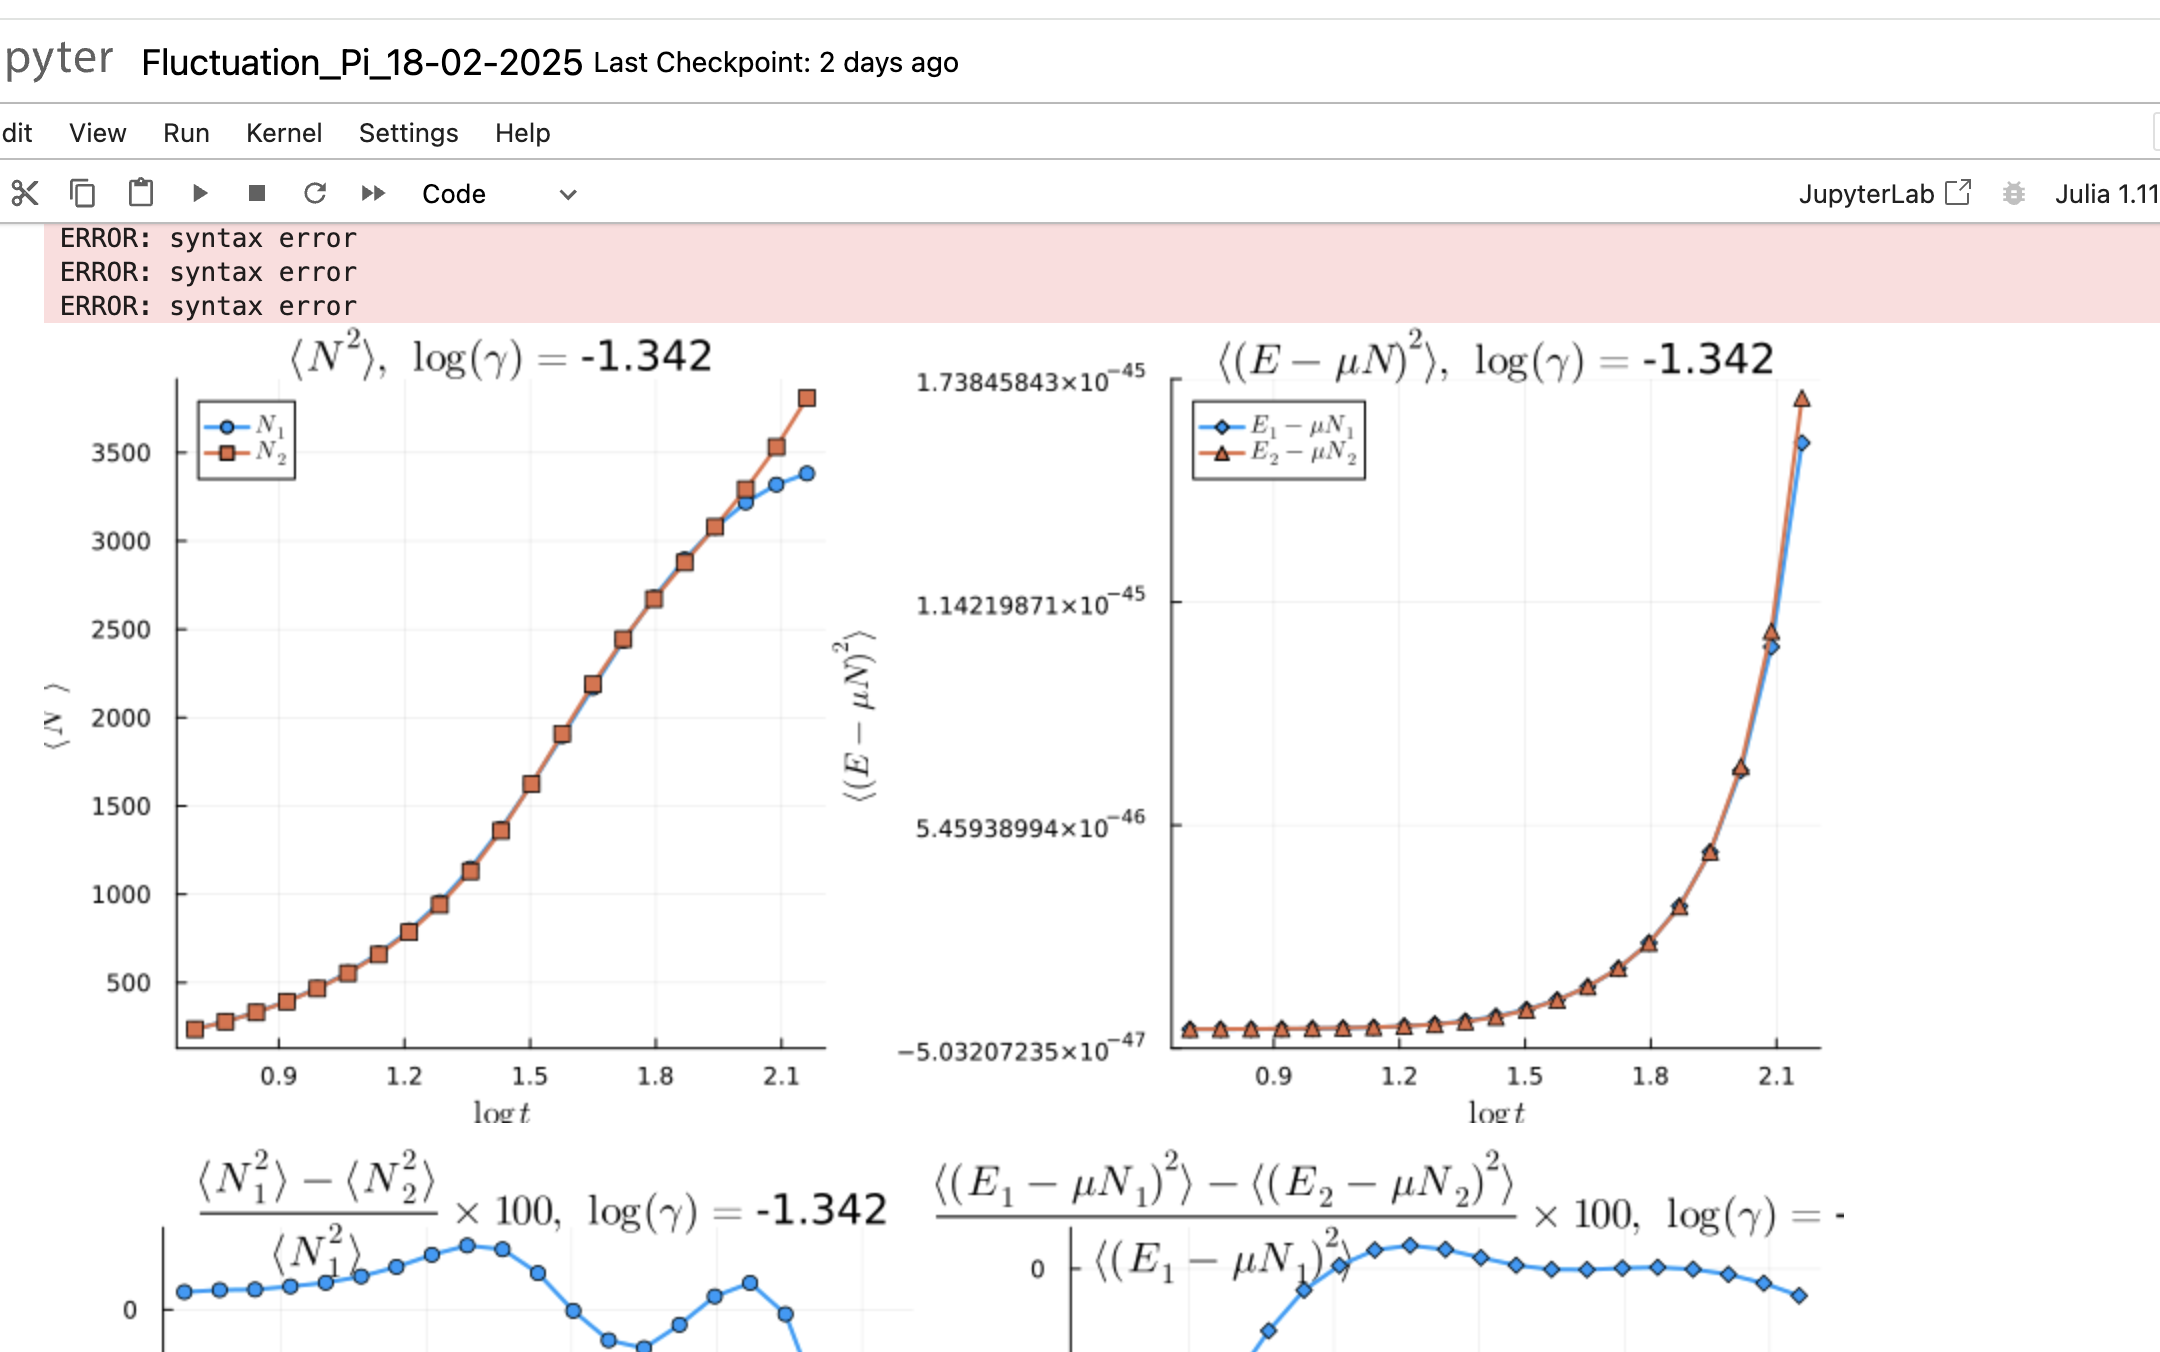
\includegraphics[width=1\textwidth]{Figures/test}

%\begin{aff}
%Donc une a l'ordre un en $\delta \theta (\operator{A}^{(0)})^{-1} %\operator{V}$ 

%\begin{eqnarray*}
%	\langle \delta \Pi ( \theta) \delta \Pi ( \theta') \rangle & = &  ( (\Pi^c_s - \Pi^c)\Pi^c/\Pi^c_s ) ( \theta ) \delta_{\theta, \theta'}/\delta \theta + \mathscr{F}(\theta , \theta' ) ,	
%\end{eqnarray*}

%avec 

%\begin{eqnarray*}
%	\mathscr{F}(\theta , \theta' ) & = & \left [ (\Pi^c_s - \Pi^c )( \theta)  +  (\Pi^c_s - \Pi^c ) ( \theta' )\right ] \frac{\Pi^c}{\Pi^c_s}(\theta)\frac{\Pi^c}{\Pi^c_s}(\theta') \frac{ \Delta( \theta'- \theta )}{ 2 \pi }\\
%	&&  - \left [ (\Pi^c_s - \Pi^c )( \theta)   (\Pi^c_s - \Pi^c ) ( \theta' )\right ] \frac{\Pi^c}{\Pi^c_s}(\theta)\frac{\Pi^c}{\Pi^c_s}(\theta')\int d\theta'' \left (   \frac{ \Pi^c/\Pi^c_s}{\Pi^c_s - \Pi^c} \right )(\theta'') \frac{\Delta(\theta''- \theta)}{2 \pi}\frac{\Delta(\theta''- \theta')}{2 \pi}  	
%\end{eqnarray*}
%\end{aff}



 










		